\documentclass[a4paper,12pt]{article}
\usepackage[T1]{fontenc}
\usepackage{rotating}
\usepackage{lscape}
\usepackage{amssymb,amsmath,amssymb}
\usepackage[stable]{footmisc}
\usepackage{lmodern}
\usepackage{libertine}
\usepackage[libertine]{newtxmath}
\usepackage[scale=0.825]{FiraMono}
\usepackage[authoryear]{natbib}
\usepackage{babelbib}
\usepackage{booktabs, makecell, longtable}
\usepackage[usenames,dvipsnames]{xcolor}
\definecolor{darkblue}{rgb}{0.0,0.0,0.55}
\setcitestyle{aysep={}} 
\usepackage{etoolbox}
\makeatletter
\patchcmd{\NAT@citex}
  {\@citea\NAT@hyper@{%
	 \NAT@nmfmt{\NAT@nm}%
	 \hyper@natlinkbreak{\NAT@aysep\NAT@spacechar}{\@citeb\@extra@b@citeb}%
	 \NAT@date}}
  {\@citea\NAT@nmfmt{\NAT@nm}%
   \NAT@aysep\NAT@spacechar\NAT@hyper@{\NAT@date}}{}{}
\patchcmd{\NAT@citex}
  {\@citea\NAT@hyper@{%
	 \NAT@nmfmt{\NAT@nm}%
	 \hyper@natlinkbreak{\NAT@spacechar\NAT@@open\if*#1*\else#1\NAT@spacechar\fi}%
   {\@citeb\@extra@b@citeb}%
	 \NAT@date}}
  {\@citea\NAT@nmfmt{\NAT@nm}%
   \NAT@spacechar\NAT@@open\if*#1*\else#1\NAT@spacechar\fi\NAT@hyper@{\NAT@date}}
  {}{}
\makeatother
\usepackage{setspace}
\usepackage[top=2cm,bottom=2cm,left=2cm,right=2cm]{geometry}
\usepackage{rotating}
\usepackage{caption}
\usepackage{adjustbox}
\usepackage{pgf}
\usepackage{tikz}
\usetikzlibrary{arrows}
\usetikzlibrary{positioning}
\usepackage{dcolumn}
\usepackage{float}
\floatplacement{figure}{H}
\usepackage{pgf}
\usepackage{tikz}
\usetikzlibrary{arrows}
\usetikzlibrary{positioning}
\usepackage{mathtools}
\usepackage{caption}
\usepackage{ifthen}
\usepackage[UKenglish]{babel}
\usepackage[UKenglish]{isodate}
\cleanlookdateon
\exhyphenpenalty=1000
\hyphenpenalty=1000
\widowpenalty=1000
\clubpenalty=1000
\usepackage[backref,pagebackref]{hyperref}
\renewcommand*{\backref}[1]{}
\renewcommand*{\backrefalt}[4]{%
	\ifcase #1 (Not cited.)%
	\or        Cited on page~#2.%
	\else      Cited on pages~#2.%
	\fi}
\renewcommand{\backreftwosep}{ and~}
\renewcommand{\backreflastsep}{ and~}
	
\hypersetup{pdftitle={What Drives State-Sponsored Violence?: Evidence from Extreme Bounds Analysis and Ensemble Learning Models},
		pdfauthor={Danilo Freire and Gary Uzonyi},
		pdfborder={0 0 0},
		breaklinks=false,
		linkcolor=Mahogany,
		citecolor=Mahogany,
		urlcolor=darkblue,
		colorlinks=true}
	
\title{Appendix for \textit{What Drives State-Sponsored Violence?: Evidence from Extreme Bounds Analysis and Ensemble Learning Models}}
	
\author{Danilo Freire\thanks{Postdoctoral Research Associate, The Political Theory Project, Brown University, 8 Fones Alley, Providence, RI 02912,  \href{mailto:danilofreire@gmail.com}{\texttt{danilofreire@gmail.com}}, \href{http://danilofreire.com}{\texttt{http://danilofreire.com}}. Corresponding author.} \and Gary Uzonyi\thanks{Assistant Professor, Department of Political Science; Research Fellow, Howard H. Baker Jr. Center for Public Policy, University of Tennessee, 1640 Cumberland Ave, Knoxville, TN 37996, \href{mailto:guzonyi@utk.edu}{\texttt{guzonyi@utk.edu}}, \href{https://sites.google.com/site/uzonyigary/}{\texttt{https://sites.google.com/site/uzonyigary}}.}}

\date{\today}

\begin{document}
\maketitle

{\hypersetup{linkcolor=black}
\tableofcontents
}

\newpage
	
\section{Introduction}
\label{sec:intro}
	
\doublespacing
	
This appendix contains all required information to replicate the numerical analyses presented in ``What Drives State-Sponsored Violence?: Evidence from Extreme Bounds Analysis and Ensemble Learning Models.'' \texttt{R} code can be found in subsection \ref{sec:mk-code} below. The data are available on GitHub at \href{https://github.com/danilofreire/mass-killings}{\texttt{https://github.com/danilofreire/mass-killings}}. The repository also includes the complete for both extreme bounds analysis and the random forests models. They are available in the \texttt{models} folder. We used \texttt{R} version 3.5.1 (2018-07-02) and macOS High Sierra (10.13.6) to perform all statistical calculations.

\section{Variable Selection}
\label{sec:mk-vs}

We employ some criteria to select our explanatory variables. First, we included only published articles in our sample. Although working papers and policy may also provide important insights about the onset of mass killings, we believe that peer-reviewed research is probably better suited for our purposes. Also, we included only papers that use regression methods on a global sample and were published from 1995 to 2015. Our final sample comprises 45 articles: \citet{anderton2015new}, \citet{balcells2010rivalry, balcells2011continuation}, \citet{besanccon2005relative}, \citet{bulutgil2015social}, \citet{bundervoet2009livestock}, \citet{clayton2016civilianizing}, \citet{colaresi2008kill}, \citet{downes2006desperate, downes2007restraint},  \citet{easterly2006development}, \citet{eck2007one}, \citet{esteban2015strategic}, \citet{fazal2015particular}, \citet{fjelde2014weakening}, \citet{goldsmith2013forecasting}, \citet{harff2003no}, \citet{joshi2017kills}, \citet{kim2010makes}, \citet{kim2016revolutionary}, \citet{kisangani2007political}, \citet{koren2017means}, \citet{krain1997state}, \citet{manekin2013violence}, \citet{mcdoom2013killed,mcdoom2014predicting}, \citet{melander2009new}, \citet{montalvo2008discrete}, \citet{pilster2016differentiation}, \citet{querido2009state}, \citet{raleigh2012violence}, \citet{rost2013will}, \citet{rummel1995democracy}, \citet{schneider2013accounting}, \citet{siroky2015empire}, \citet{stanton2015regulating}, \citet{sullivan2012blood}, \citet{tir2008domestic}, \citet{ulfelder2008assessing}, \citet{ulfelder2012forecasting}, \citet{uzonyi2015civil, uzonyi2016domestic} \citet{valentino2004draining}, \citet{valentino2006covenants}, \citet{verpoorten2012leave}, \citet{wayman2010explaining}, \citet{wig2016local}, and \citet{yanagizawa2014propaganda}.

We find that in those 45 studies scholars made use of nearly 180 measurements to capture roughly 30 key concepts related to threat and costs of mass killings. To be added to our models, a variable should appear in at least two articles. The covariates are summarised in table \ref{tab:mk-vs}. A complete list of variables is available at \href{https://github.com/danilofreire/mass-killings/data}{\texttt{https://github.com/danilofreire/mass-killings/data}}.

\begin{table}[!htbp] \centering 
  \caption{Independent Variables} 
  \label{tab:mk-vs} 
\footnotesize
\begin{tabular}{@{\extracolsep{5pt}}lcc} 
\\[-1.8ex]\hline 
\hline \\[-1.8ex] {Variable} & \multicolumn{1}{c}{Coded} & \multicolumn{1}{c}{Source}\\ 
\hline \\[-1.8ex] 
Assassination & Dichotomous & \citet{banks1999cross} \\ 
CINC & Continuous & \citet{cow2017cinc}\\ 
Coup d'état & Dichotomous & \citet{marshall2017pitf}  \\ 
COW civil war onset & Dichotomous & \citet{cow2017cinc,singer1988reconstructing} \\ 
COW civil war ongoing & Dichotomous & \citet{cow2017cinc,singer1988reconstructing} \\ 
Democracy (Polity IV $\geq 6$) & Dichotomous  & Authors' own calculations \\ 
Discriminated dummy & Dichotomous & \citet{cederman2010ethnic}\\ 
Discriminated population & Continuous & \citet{cederman2010ethnic} \\ 
Ethnic diversity (ELF) & Continuous & \citet{fearon2003ethnicity} \\ 
Ethnic war start & Dichotomous & \citet{cederman2010ethnic} \\ 
Ethnic war ongoing & Dichotomous & \citet{cederman2010ethnic} \\ 
Excluded population & Continuous & \citet{cederman2010ethnic} \\ 
Interstate war & Dichotomous & \citet{singer1988reconstructing,cow2017cinc} \\ 
Guerrilla & Dichotomous & \citet{balcells2014does}\\ 
Military expenditure & Continuous & \citet{cow2017cinc} \\ 
Military personnel & Continuous & \citet{cow2017cinc} \\ 
Militias & Dichotomous & \citet{carey2013states} \\ 
Mountainous Terrain & Continuous & \citet{fearon2003ethnicity} \\ 
Physical integrity & Continuous & \citet{cingranelli2010cingranelli}\\ 
Polarisation (all groups/main group) & Continuous &  Authors' own calculations \\ 
Polarisation (all groups/population) & Continuous &  Authors' own calculations  \\ 
Polarisation (included groups/population) & Continuous &  Authors' own calculations  \\ 
Polarisation (included groups/main group) & Continuous &  Authors' own calculations  \\ 
Polity IV & Continuous & \citet{marshall2017pitf}\\ 
Polity IV squared & Continuous & Authors' own calculations \\ 
Population & Continuous & \citet{gleditsch2002expanded} \\
Post-Cold War & Dichotomous & Authors' own calculations \\ 
Real GDP & Continuous & \citet{gleditsch2002expanded} \\ 
Real GDP per capita & Continuous & \citet{gleditsch2002expanded} \\ 
Real GDP per capita (log) & Continuous & Authors' own calculations  \\ 
Regime transition & Continuous & Authors' own calculations \\ 
Riot & Dichotomous & \citet{banks1999cross}\\ 
Total battle deaths & Continuous & \citet{lacina2005monitoring} \\  
Total trade & Continuous & \citet{cow2017cinc} \\ 
Trade dependence (total trade/real GDP) & Continuous & Authors' own calculations \\ 
UCDP civil war onset & Dichotomous & \citet{allansson2017organized,gleditsch2002armed} \\ 
UCDP civil war ongoing & Dichotomous & \citet{allansson2017organized,gleditsch2002armed} \\ 
Urban population (percentage) & Continuous & \citet{cow2017cinc} \\ 
Years since last mass killing & Continuous & Authors' own calculations \\ 
War with territory aims & Dichotomous & \citet{allansson2017organized,gleditsch2002armed} \\ 
\hline \\[-1.8ex] 
\end{tabular} 
\end{table} 

\newpage

\section{Descriptive Statistics}
\label{sec:mk-ds}

\begin{table}[!htbp] \centering 
  \caption{Descriptive Statistics} 
  \label{tab:mk-ds} 
\footnotesize 
\begin{tabular}{@{\extracolsep{5pt}}lccccc} 
\\[-1.8ex]\hline 
\hline \\[-1.8ex] 
Statistic & \multicolumn{1}{c}{N} & \multicolumn{1}{c}{Mean} & \multicolumn{1}{c}{St. Dev.} & \multicolumn{1}{c}{Min} & \multicolumn{1}{c}{Max} \\ 
\hline \\[-1.8ex] 
Country code & 9,162 & 452.84 & 247.74 & 2 & 950 \\ 
Year & 9,162 & 1,983.56 & 18.77 & 1,945 & 2,013 \\ 
Genocide/politicide onset & 8,933 & 0.005 & 0.07 & 0 & 1\\ 
Mass killing onset & 9,162 & 0.01 & 0.11 & 0 & 1 \\ 
&&&&&\\
\textit{Independent Variables} & & & & \\
&&&&&\\
Assassination dummy & 8,991 & 0.08 & 0.27 & 0 & 1 \\ 
CINC & 8,767 & 0.01 & 0.02 & 0.00 & 0.38 \\ 
Coup dummy & 8,587 & 0.05 & 0.21 & 0 & 1 \\ 
COW civil war onset & 8,160 & 0.01 & 0.12 & 0 & 1 \\ 
COW civil war ongoing & 8,160 & 0.07 & 0.25 & 0 & 1 \\ 
Democracy dummy & 8,991 & 0.37 & 0.48 & 0 & 1 \\ 
Discriminated dummy & 6,981 & 0.35 & 0.48 & 0 & 1 \\ 
Discriminated population & 6,981 & 0.06 & 0.15 & 0.00 & 0.98 \\ 
Ethnic diversity (ELF) & 6,981 & 0.41 & 0.31 & 0 & 1 \\ 
Ethnic war start & 7,760 & 0.01 & 0.12 & 0 & 1 \\ 
Ethnic war ongoing & 7,760 & 0.11 & 0.31 & 0 & 1 \\ 
Excluded population & 6,981 & 0.16 & 0.22 & 0.00 & 0.98 \\ 
Interstate war & 8,159 & 0.04 & 0.19 & 0 & 1 \\ 
Guerrilla dummy & 714 & 0.81 & 0.40 & 0 & 1 \\ 
Military expenditure & 8,290 & 4,607,120 & 27,785,906 & 0 & 693,600,000 \\ 
Military personnel & 8,620 & 176.70 & 520.90 & 0 & 12,500 \\ 
Militias & 4,097 & 0.22 & 0.42 & 0 & 1 \\ 
Mountainous Terrain & 7,358 & 2.14 & 1.43 & 0.00 & 4.56 \\ 
Physical integrity & 4,499 & 4.73 & 2.31 & 0 & 8 \\ 
Polarisation (all groups/main group) & 6,981 & 0.70 & 0.26 & 0.05 & 1 \\ 
Polarisation (all groups/population) & 6,981 & 0.63 & 0.32 & 0 & 1 \\ 
Polarisation (included groups/population) & 5,610 & 0.64 & 0.32 & 0 & 1 \\ 
Polarisation (included groups/main group) & 6,981 & 0.23 & 0.35 & 0 & 1 \\ 
Polity IV & 8,558 & 0.42 & 7.50 & $-$10 & 10 \\ 
Polity IV squared & 8,558 & 56.35 & 32.59 & 0 & 100 \\ 
Population & 8,293 & 32,993.61 & 112,886.40 & 118.21 & 1,324,353.00 \\
Post-Cold War & 8,991 & 0.40 & 0.49 & 0 & 1 \\ 
Real GDP & 8,293 & 215,317.70 & 804,827.20 & 129.68 & 13,193,478.00 \\ 
Real GDP per capita & 8,293 & 8,104.20 & 18,376.73 & 132.82 & 632,239.50 \\ 
Real GDP per capita (log) & 8,293 & 8.25 & 1.20 & 4.89 & 13.36 \\ 
Regime transition & 1,221 & $-$4.24 & 41.50 & $-$77 & 99 \\ 
Riot dummy & 8,991 & 0.16 & 0.36 & 0 & 1 \\ 
Total battle deaths & 714 & 6,050.86 & 24,404.78 & 100 & 350,000 \\  
Total trade & 8,174 & 53,804.01 & 222,209.90 & 0.80 & 4,825,363.00 \\ 
Trade dependence & 7,670 & 0.26 & 0.69 & 0.0001 & 22.11 \\ 
UCDP civil war onset & 8,733 & 0.02 & 0.14 & 0 & 1 \\ 
UCDP civil war ongoing & 8,733 & 0.15 & 0.36 & 0 & 1 \\ 
Urban population (percentage) & 8,767 & 0.22 & 0.17 & 0.00 & 1.51 \\ 
Years since last mass killing & 9,162 & 23.81 & 17.71 & 0 & 68 \\ 
War with territory aims & 8,924 & 0.07 & 0.26 & 0 & 1 \\ 
\hline \\[-1.8ex] 
\end{tabular} 
\raggedright{\newline \textit{Note}: All independent variables were lagged one year.}
\end{table} 
\normalsize

\newpage

\section{Extreme Bounds Analysis}
\label{sec:mk-ebae}

\subsection{Main Model}

We present a series of histograms with the coefficients' distribution of all variables in the main EBA model. There are 36 variables in total, seven of which are robust: Log GDP per capita, post-Cold War period, onset and ongoing civil wars (measured by the UCDP), previous riots, ethnic diversity and the squared term of the Polity IV index.

\vspace{1cm}

\begin{table}[H]
\centering
\begin{tabular}{lrrrrr}
\hline
\textbf{Variable} & \textbf{Avg. $\beta$} & \textbf{Avg. SE} & \textbf{$\%$ Sig.} & \textbf{CDF(0)} & \textbf{Models} \\ \hline
\textit{Base variables} &  &  &  &  &  \\
Log GDP per capita & -0.0091 & 0.0052 & 76.055 & 0.9335 & 226707 \\
 &  &  &  &  &  \\
\textit{Additional variables} &  &  &  &  &  \\
Post-Cold War years & -0.0133 & 0.0085 & 72.845 & 0.9472 & 35614 \\
UCDP civil war onset & 0.0529 & 0.0321 & 52.378 & 0.9441 & 20854 \\
Previous riots & 0.0140 & 0.0100 & 56.242 & 0.9216 & 35614 \\
UCDP ongoing civil war & 0.0172 & 0.0115 & 65.652 & 0.9092 & 20854 \\
Ethnic diversity (ELF) & 0.0184 & 0.0137 & 56.674 & 0.9050 & 35614 \\
Polity IV squared & -0.0002 & 0.0001 & 61.206 & 0.9031 & 35614 \\ \hline
\end{tabular}
\caption{Extreme Bounds Analysis -- Mass killings}
\label{tab:mk}
\end{table}

\begin{figure}[H]
    \centering
    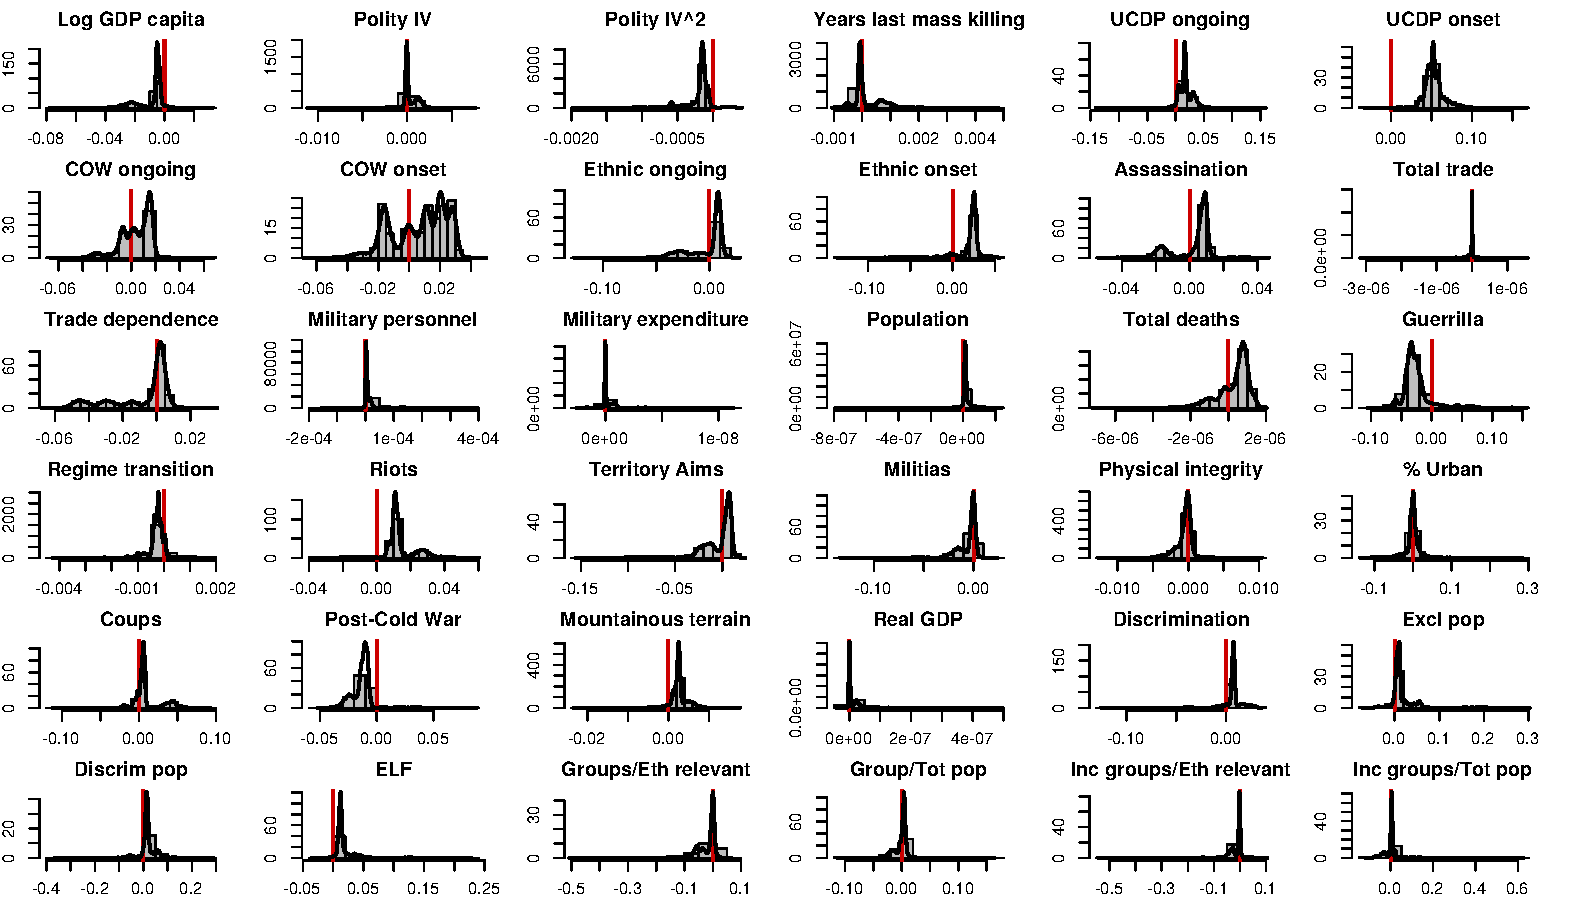
\includegraphics[width=.98\textheight,angle=90]{images/mk.pdf}
    \caption{Extreme Bounds Analysis -- Mass Killings}
    \label{fig:mk}
\end{figure}

\subsection{Genocides during Civil Wars}
\label{sec:civil-wars}

Next, we discuss genocides that occur during wartime. We use three covariates that denote ongoing civil conflicts: one by the Uppsala Conflict Data Program \citep{allansson2017organized,gleditsch2002armed}, another by the Correlates of War \citep{sarkees2010resort}, and a third indicating the onset of ethnic conflict as coded by \citet{cederman2010ethnic}. The variables that reach significance in this set of models below are notably different from those obtained in the main estimation. This result provides evidence that mass violence during wartime time follows a separate logic from state killings in peacetime.

\vspace{1cm}

\begin{table}[H]
\centering
\begin{tabular}{lrrrrr}
\hline
\textbf{Variable} & \textbf{Avg. $\beta$} & \textbf{Avg. SE} & \textbf{$\%$ Sig.} & \textbf{CDF(0)} & \textbf{Models} \\ \hline
\textit{UCDP data} &  &  &  &  &  \\
Territory aims & -0.044 & 0.019 & 74.997 & 0.9804 & 17902 \\
Post-Cold War years & -0.038 & 0.019 & 66.574 & 0.9222 & 17902 \\
 &  &  &  &  &  \\
\textit{COW data} &  &  &  &  &  \\
Physical integrity & 0.024 & 0.013 & 66.674 & 0.9564 & 17902 \\
Militias & -0.099 & 0.048 & 73.104 & 0.9490 & 17902 \\
Years since last mass killing & 0.006 & 0.002 & 88.208 & 0.9472 & 101583 \\
Previous riots & 0.078 & 0.041 & 65.412 & 0.9348 & 17902 \\
Ethnic diversity (ELF) & 0.095 & 0.062 & 48.615 & 0.9000 & 17902 \\
 &  &  &  &  &  \\
\textit{Cederman et al. data} &  &  &  &  &  \\
Territory aims & -0.051 & 0.026 & 74.288 & 0.9167 & 17902 \\
Militias & -0.050 & 0.035 & 52.240 & 0.9101 & 17902 \\ \hline
\end{tabular}
\caption{EBA -- Mass Killings during Civil Wars}
\label{tab:ucdp1}
\end{table}

\begin{figure}
    \centering
    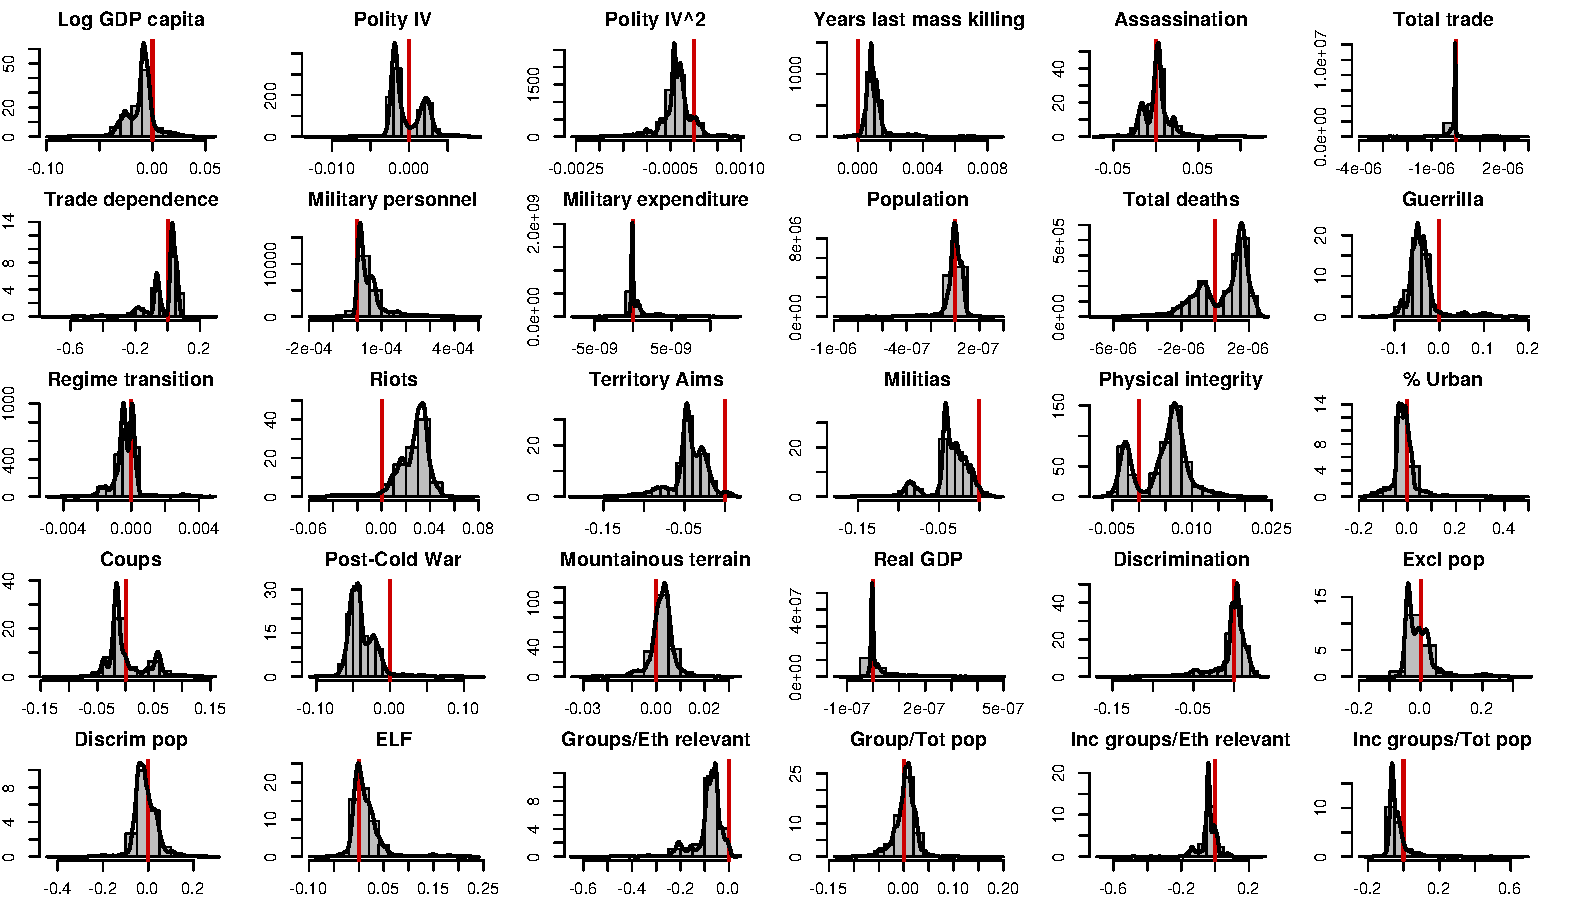
\includegraphics[width=.98\textheight,angle=90]{images/mk-ucdp.pdf}
    \caption{EBA -- Mass Killings during Civil Wars (UCDP Data)}
    \label{fig:mk-ucdp}
\end{figure}

\begin{figure}
    \centering
    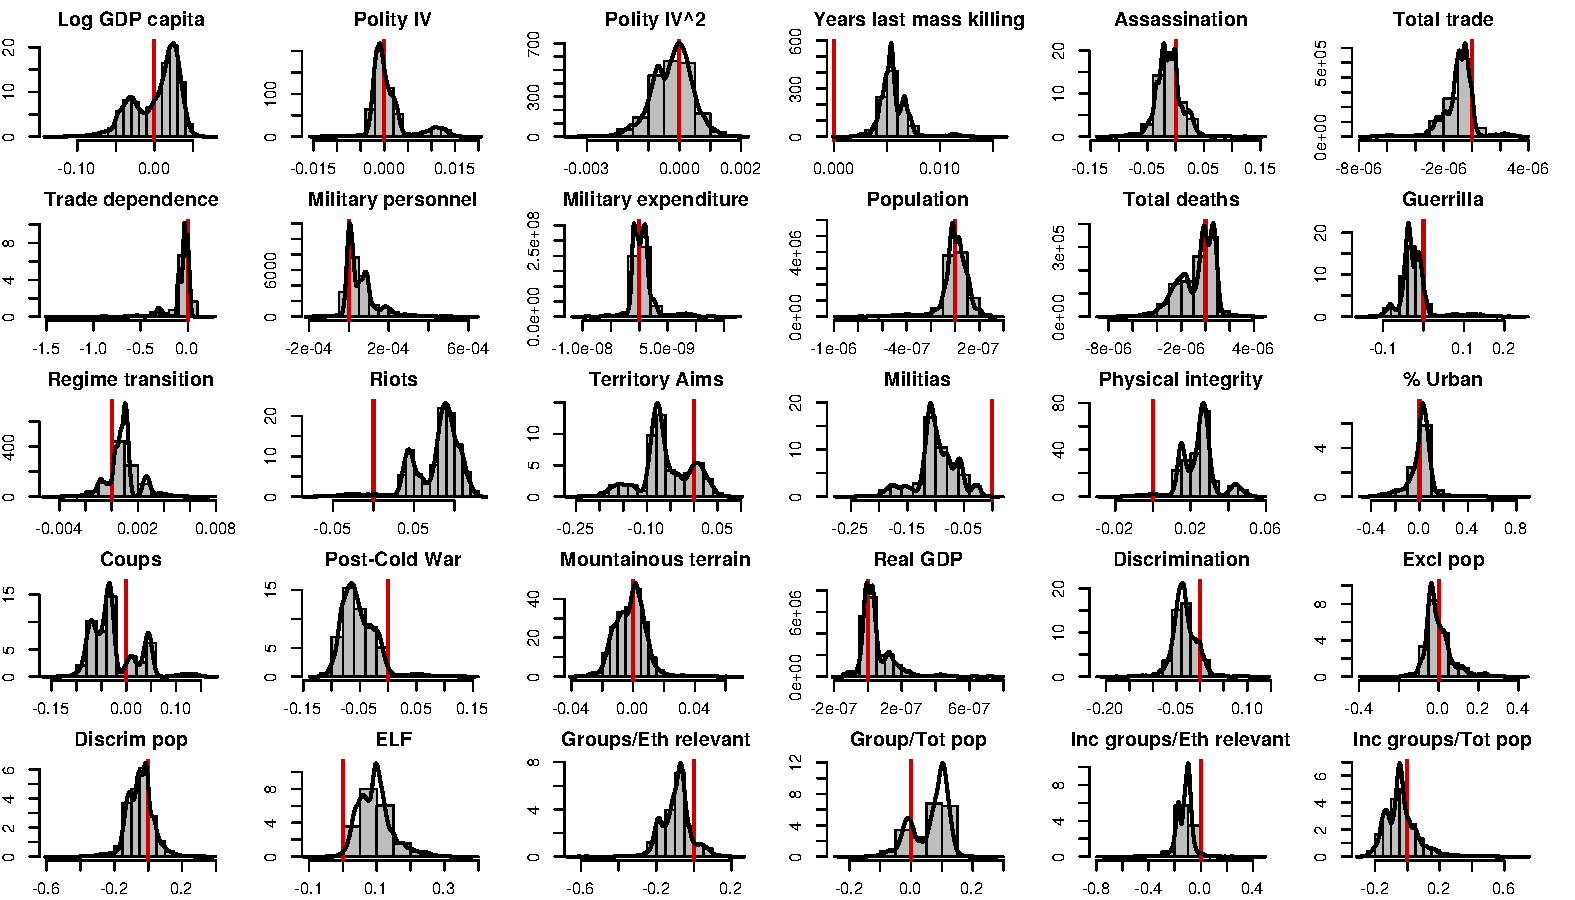
\includegraphics[width=.98\textheight,angle=90]{images/mk-cow.pdf}
    \caption{EBA -- Mass Killings during Civil Wars (COW Data)}
    \label{fig:mk-cow}
\end{figure}

\begin{figure}
    \centering
    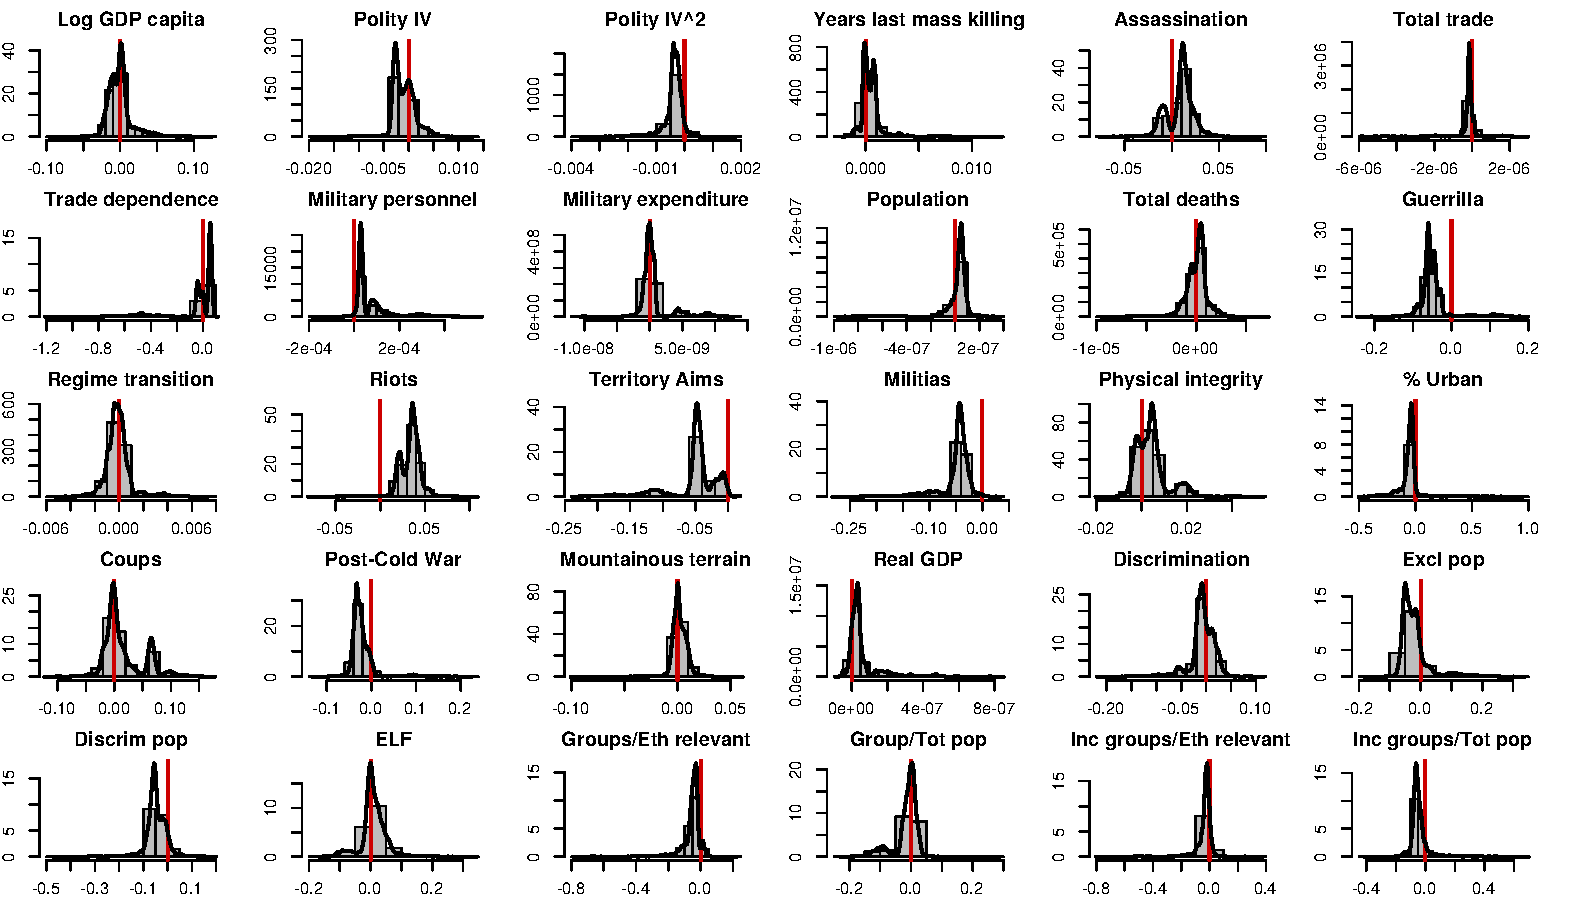
\includegraphics[width=.98\textheight,angle=90]{images/mk-eth.pdf}
    \caption{EBA -- Mass Killings during ethnic civil wars (Cederman et al. Data)}
    \label{fig:mk-eth}
\end{figure}

\subsection{Alternative Number of Variables}

The models below are based on 50,000 random draws from the full set of all possible regression models. \citet[819]{salaimartin2004determinants} argue that random sampling produces unbiased estimates of the regression coefficients with low computational time. The models presented in section \ref{sec:results4}, however, include the full set of possible regressions.

The following table shows the results of an EBA with 3 variable combinations per model. The results are very similar to those reported above.

\vspace{1cm}

\begin{table}[H]
\centering
\begin{tabular}{lrrrrr}
\hline
\textbf{Variable} & \textbf{Avg. $\beta$} & \textbf{Avg. SE} & \textbf{$\%$ Sig.} & \textbf{CDF(0)} & \textbf{Models} \\ \hline
\textit{Base variables} &  &  &  &  &  \\
Log GDP per capita & 0.0082 & 0.0043 & 81.439 & 0.9504 & 40677 \\
 &  &  &  &  &  \\
\textit{Additional variables} &  &  &  &  &  \\
Post-Cold War years & -0.0121 & 0.0069 & 77.804 & 0.9609 & 5064 \\
UCDP civil war onset & 0.0523 & 0.0292 & 62.561 & 0.9574 & 3304 \\
Previous riots &0.0134 & 0.0084 & 65.936 & 0.9401 & 5064 \\
UCDP ongoing civil war & 0.0177 & 0.0094 & 72.367 & 0.9372 & 3304 \\
Polity IV squared & -0.0002 & 0.0001 & 66.035 & 0.9268 & 5064 \\ 
Ethnic diversity (ELF) & 0.0162 & 0.0110 & 70.794 & 0.9266 & 5064 \\\hline
\end{tabular}
\caption{EBA -- 3 Variables}
\label{tab:mk-3vars}
\end{table}

\begin{figure}
    \centering
    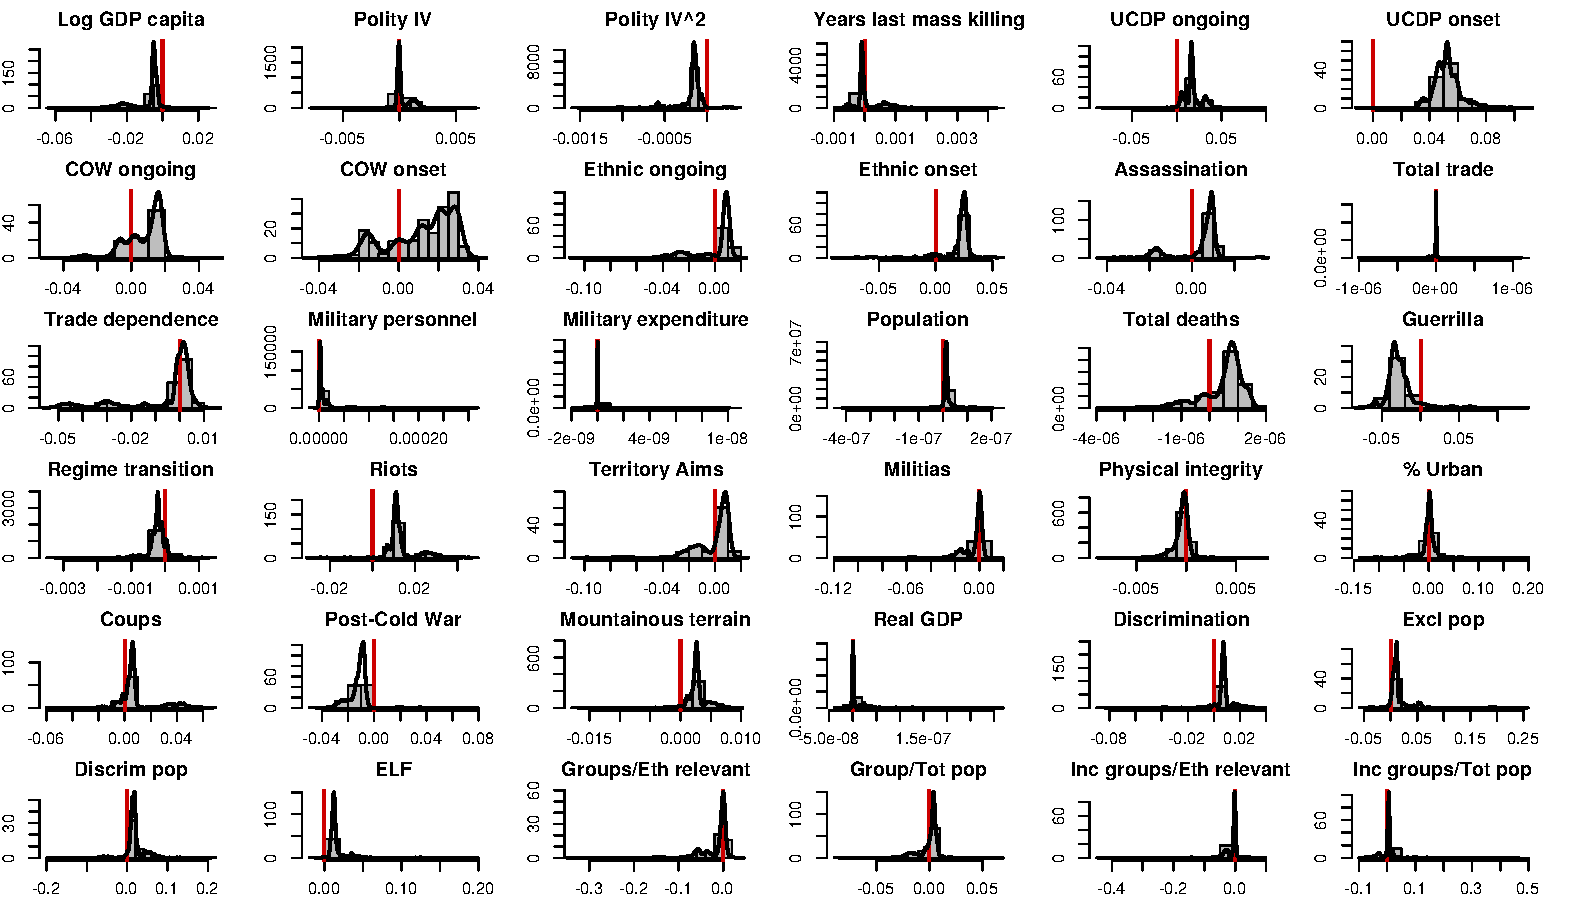
\includegraphics[width=.98\textheight,angle=90]{images/mk-3vars.pdf}
    \caption{EBA -- 3 Variables}
    \label{fig:mk-3vars}
\end{figure}

Table \ref{tab:mk-5vars} presents the results for models with up 5 variables in each regressions. In contrast with our main EBA model, the indicators of UCDP ongoing civil wars, ethnic diversity, and Polity IV square drop out of significance. Their individual CDFs(0) are about 0.88, just marginally below our specified threshold of 0.9.

\vspace{1cm}

\begin{table}[!htpb]
\centering
\begin{tabular}{lrrrrr}
\hline
\textbf{Variable} & \textbf{Avg. $\beta$} & \textbf{Avg. SE} & \textbf{$\%$ Sig.} & \textbf{CDF(0)} & \textbf{Models} \\ \hline
\textit{Base variables} &  &  &  &  &  \\
Log GDP per capita & -0.010 & 0.006 & 70.806 & 0.9161 & 50000 \\
 &  &  &  &  &  \\
\textit{Additional variables} &  &  &  &  &  \\
Post-Cold War years & -0.014 & 0.010 & 68.496 & 0.9336 & 9532 \\
UCDP civil war onset & 0.053 & 0.035 & 44.784 & 0.9308 & 5100 \\
Previous riots & 0.015 & 0.012 & 47.988 & 0.9047 & 9569 \\\hline
\end{tabular}
\caption{EBA -- 5 Variables}
\label{tab:mk-5vars}
\end{table}

\begin{figure}
    \centering
    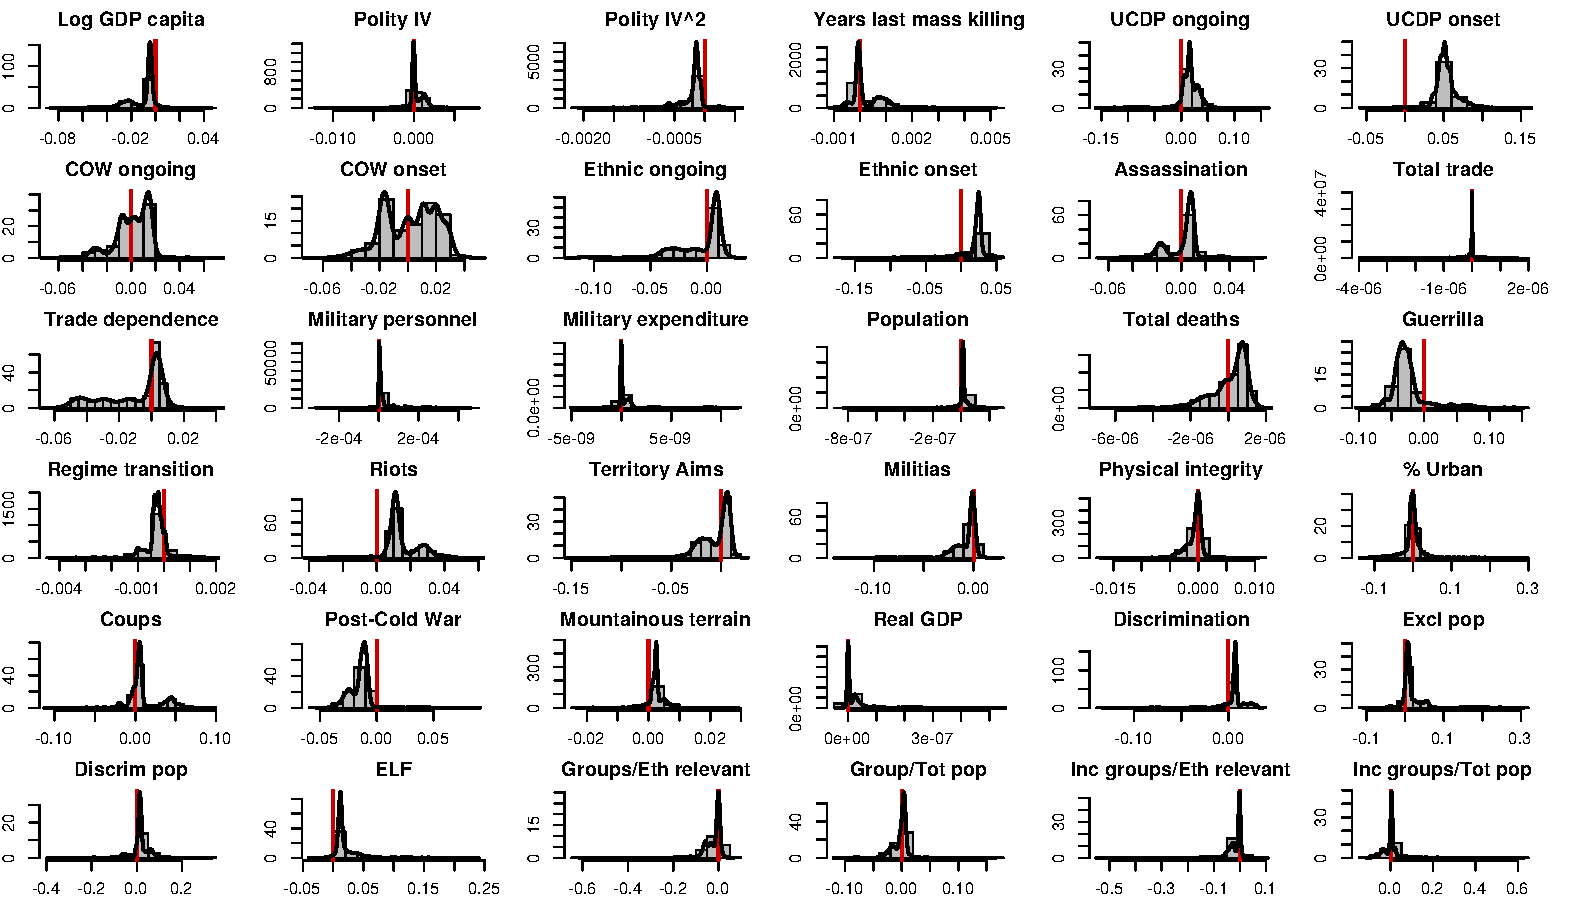
\includegraphics[width=.98\textheight,angle=90]{images/mk-5vars.pdf}
    \caption{EBA -- 5 Variables}
    \label{fig:mk-5vars}
\end{figure}

\subsection{Alternative Variance Inflation Factors}

In this subsection, we estimate EBA models with different values of Variance Inflation Factor (VIF), which is a measure of multicollinearity. There is no standard definition about what constitutes an acceptable VIF value, although researchers often use 10 as rule of thumb to indicate strong multicollinearity \citep[674]{o2007caution}. Our original model used a slightly more conservative value of 7 as a cutoff. Here, we test the same model with VIF $=$ 10 (less strict), 2.5 (more conservative), and a model without VIF restrictions. The results are essentially identical to those of the main model. In the model with no VIF restriction, however, ethnic fractionalisation fails to meet the threshold by a very small margin. The CDF(0) of that covariate is 0.897, very close to the required value of 0.9. 

\vspace{1cm}

\begin{table}[H]
\centering
\begin{tabular}{lrrrrr}
\hline
\textbf{Variable} & \textbf{Avg. $\beta$} & \textbf{Avg. SE} & \textbf{$\%$ Sig.} & \textbf{CDF(0)} & \textbf{Models} \\ \hline
\textit{Base variables} &  &  &  &  &  \\
Log GDP per capita & -0.0091 & 0.0052 & 76.354 & 0.9343 & 50000 \\
 &  &  &  &  &  \\
\textit{Additional variables} &  &  &  &  &  \\
Post-Cold War years & -0.0134 & 0.0084 & 73.540 & 0.9495 & 7929 \\
UCDP civil war onset & 0.0529 & 0.0322 & 52.141 & 0.9438 & 4553 \\
Previous riots & 0.0140 & 0.0100 & 56.433 & 0.9216 & 7772 \\
UCDP ongoing civil war & 0.0172 & 0.0113 & 66.013 & 0.9113 & 4587 \\
Ethnic diversity (ELF) & 0.0182 & 0.0136 & 56.872 & 0.9056 & 8076 \\
Polity IV squared & -0.0002 & 0.0001 & 60.791 & 0.9021 & 7835 \\ \hline
\end{tabular}
\caption{EBA -- VIF 10}
\label{tab:mk-high-vif}
\end{table}

\begin{figure}
    \centering
    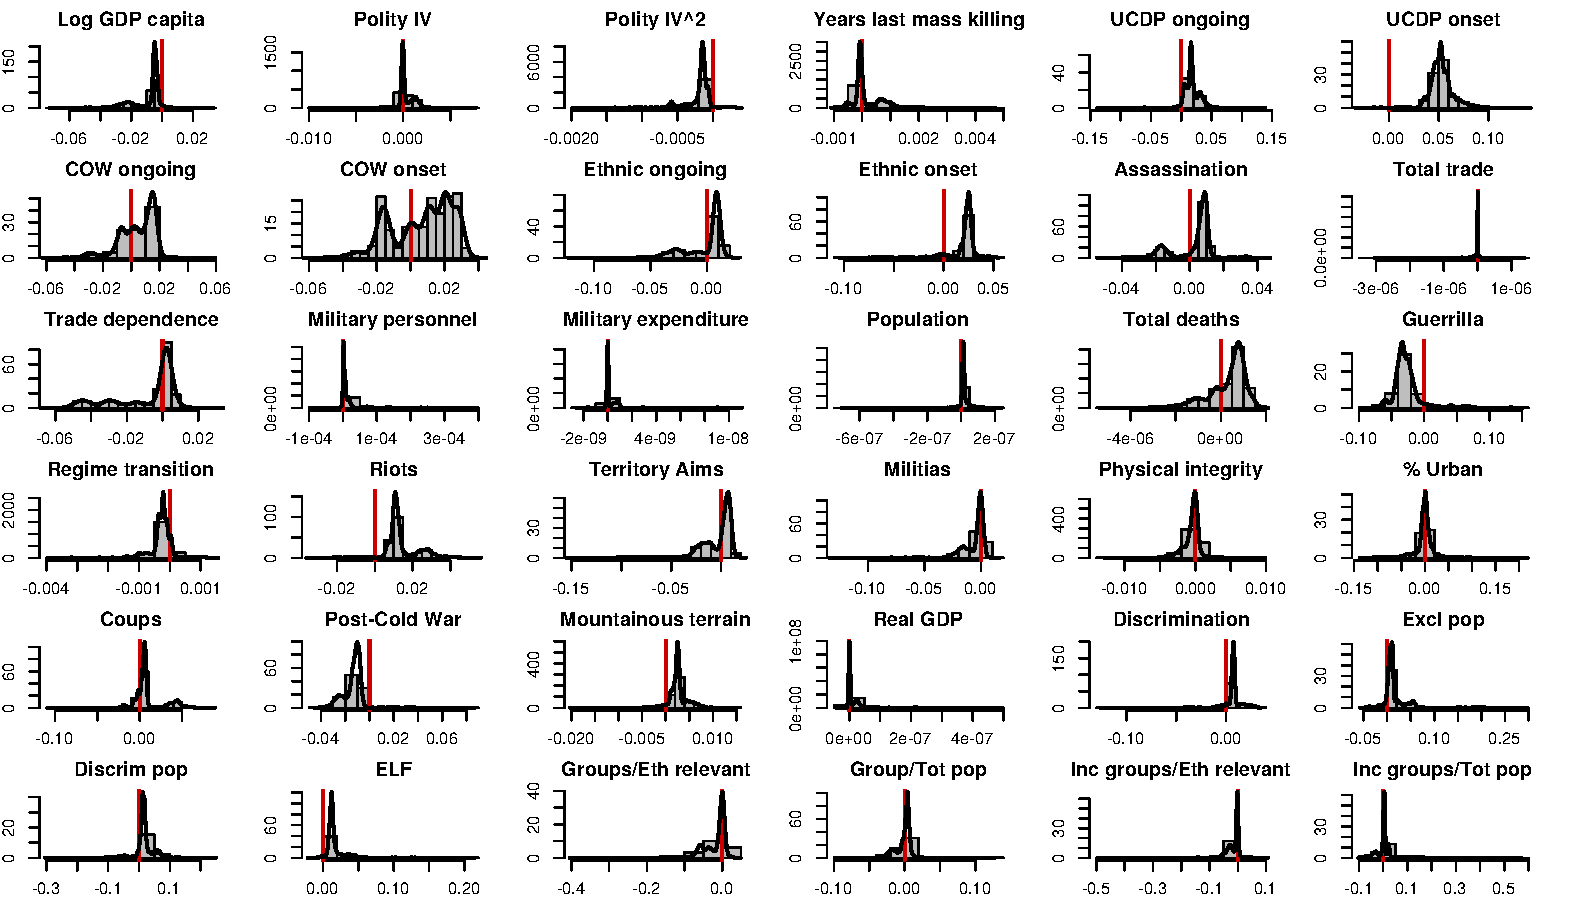
\includegraphics[width=.98\textheight,angle=90]{images/mk-high-vif.pdf}
    \caption{EBA -- VIF 10}
    \label{fig:mk-high-vif}
\end{figure}

\vspace{1cm}

\begin{table}[H]
\centering
\begin{tabular}{lrrrrr}
\hline
\textbf{Variable} & \textbf{Avg. $\beta$} & \textbf{Avg. SE} & \textbf{$\%$ Sig.} & \textbf{CDF(0)} & \textbf{Models} \\ \hline
\textit{Base variables} &  &  &  &  &  \\
Log GDP per capita & -0.0090 & 0.0051 & 76.055 & 0.9343 & 49620 \\
 &  &  &  &  &  \\
\textit{Additional variables} &  &  &  &  &  \\
Post-Cold War years & -0.0132 & 0.0084 & 72.845 & 0.9490 & 7929 \\
UCDP civil war onset & 0.0529 & 0.0322 & 52.378 & 0.9438 & 4553 \\
Previous riots & 0.0141 & 0.0101 & 56.242 & 0.9199 & 7772 \\
UCDP ongoing civil war & 0.0174 & 0.0114 & 65.652 & 0.9103 & 4587 \\
Ethnic diversity (ELF) & 0.0184 & 0.0137 & 56.674 & 0.9054 & 8076 \\
Polity IV squared & -0.0002 & 0.0001 & 61.206 & 0.90267 & 7835 \\ \hline
\end{tabular}
\caption{EBA -- VIF 2.5}
\label{tab:low-vif}
\end{table}

\begin{figure}
    \centering
    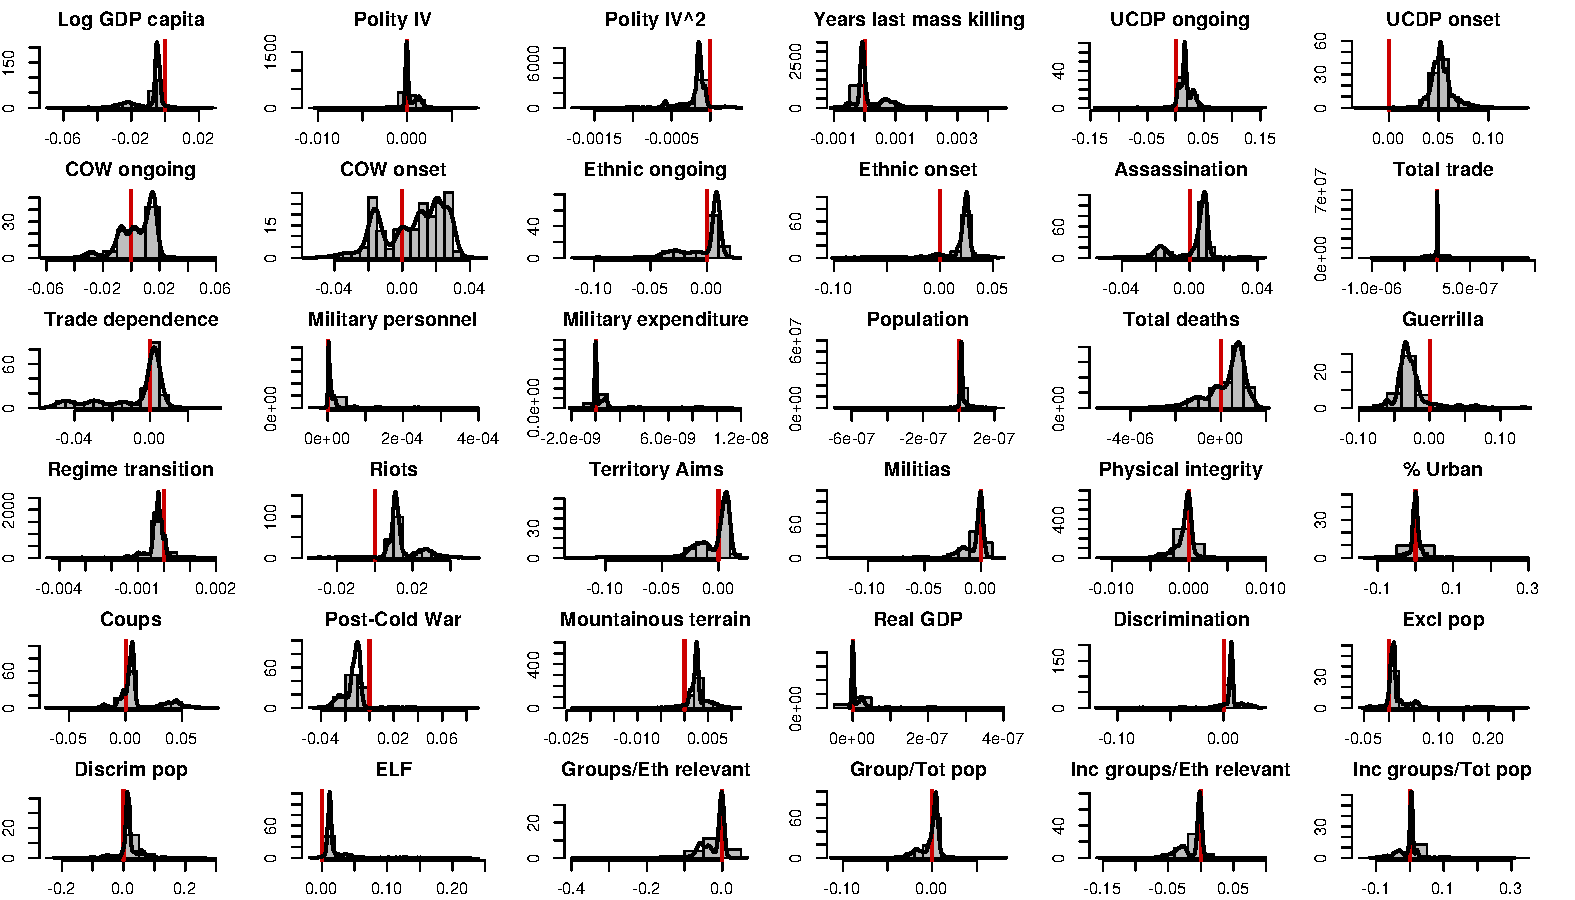
\includegraphics[width=.98\textheight,angle=90]{images/mk-low-vif.pdf}
    \caption{EBA -- VIF 2.5}
    \label{fig:mk-low-vif}
\end{figure}

\begin{table}[H]
\centering
\begin{tabular}{lrrrrr}
\hline
\textbf{Variable} & \textbf{Avg. $\beta$} & \textbf{Avg. SE} & \textbf{$\%$ Sig.} & \textbf{CDF(0)} & \textbf{Models} \\ \hline
\textit{Base variables} &  &  &  &  &  \\
Log GDP per capita & -0.0091 & 0.0052 & 75.940 & 0.9343 & 50000 \\
 &  &  &  &  &  \\
\textit{Additional variables} &  &  &  &  &  \\
Post-Cold War years & -0.0133 & 0.0085 & 72.756 & 0.9469 & 7800 \\
UCDP civil war onset & 0.0531 & 0.0321 & 53.068 & 0.9452 & 4596 \\
Previous riots & 0.0140 & 0.0101 & 56.139 & 0.9200 & 7811 \\
UCDP ongoing civil war & 0.0170 & 0.0116 & 64.487 & 0.9057 & 4497 \\
Ethnic diversity (ELF) & 0.0184 & 0.0137 & 56.814 & 0.9056 & 7808 \\
Polity IV squared & -0.0002 & 0.0001 & 60.825 & 0.9009 & 7903 \\ \hline
\end{tabular}
\caption{EBA -- No VIF Restriction}
\label{tab:mk-no-vif}
\end{table}

\begin{figure}
    \centering
    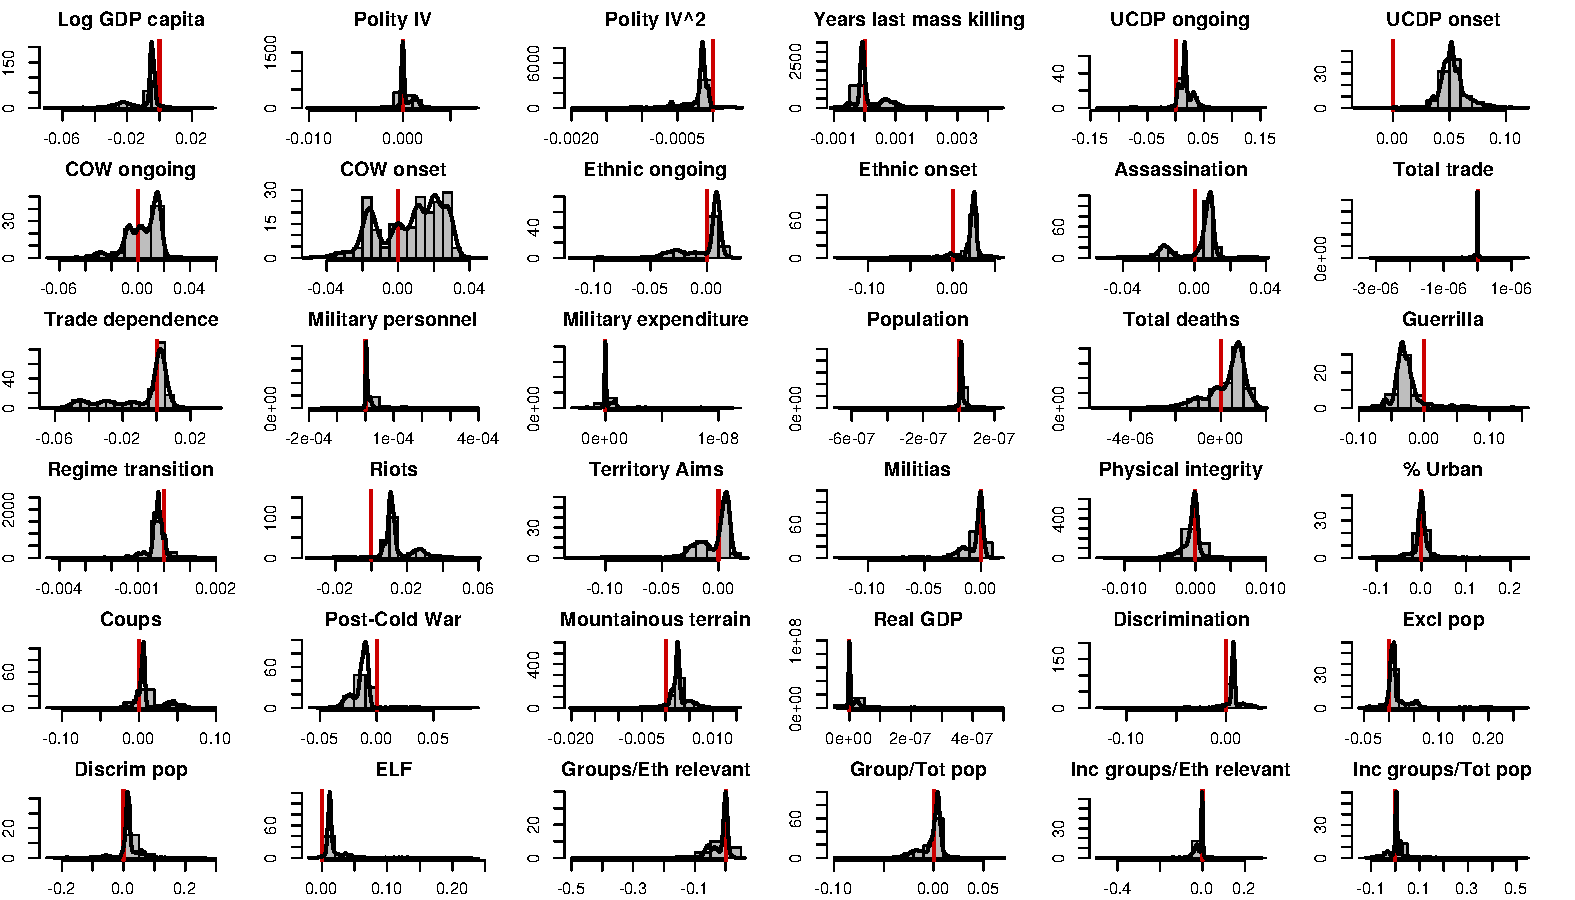
\includegraphics[width=.98\textheight,angle=90]{images/mk-no-vif.pdf}
    \caption{EBA -- No VIF restriction}
    \label{fig:mk-no-vif}
\end{figure}

\subsection{Generalised Linear Models}

We reestimate the main EBA model with logit and probit models. Logit and probit regressions may have issues of complete separation, that is, some covariates may perfectly separate zeros and ones in the outcome variable. In that case, the estimations fail to converge. We address this problem by adding a weak prior to the regression coefficients as suggested by \citet{gelman2008weakly}.\footnote{We thank Mark Bell for sharing \texttt{R} code to estimate penalised-likelihood models.} First, we scaled the non-binary variables to have a mean of 0 and a standard deviation of 0.5, then added a Cauchy distribution with centre 0 and scale 2.5. The probit regressions use a scale of $2.5 \times 1.6$, which is also recommended by the authors \citep{arm2017rpackage}. Ethnic diversity and ongoing civil wars come close to meeting our threshold values (0.88 and 0.84, respectively), and civil war onset (UCDP) has a higher percentage of significant coefficients and a high CDF(0) area than in the linear probability models.

\vspace{1cm}

\begin{table}[H]
\centering
\begin{tabular}{lrrrrr}
\hline
\textbf{Variable} & \textbf{Avg. $\beta$} & \textbf{Avg. SE} & \textbf{$\%$ Sig.} & \textbf{CDF(0)} & \textbf{Models} \\ \hline
\textit{Base variables} &  &  &  &  &  \\
Log GDP per capita & 0.434 & 0.223 & 75.570 & 0.9267 & 50000 \\
 &  &  &  &  &  \\
\textit{Additional variables} &  &  &  &  &  \\
UCDP civil war onset & 1.308 & 0.530 & 87.261 & 0.9742 & 4506 \\
Post-Cold War years & -0.911 & 0.428 & 70.456 & 0.9448 & 7890 \\
Previous riots & 0.744 & 0.38 & 66.778 & 0.9383 & 7805 \\
Polity IV squared & -0.015 & 0.008 & 68.038 & 0.9285 & 7975 \\ \hline
\end{tabular}
\caption{EBA -- Logistic Regression}
\label{tab:mk-logit}
\end{table}

\newpage

\begin{figure}
    \centering
    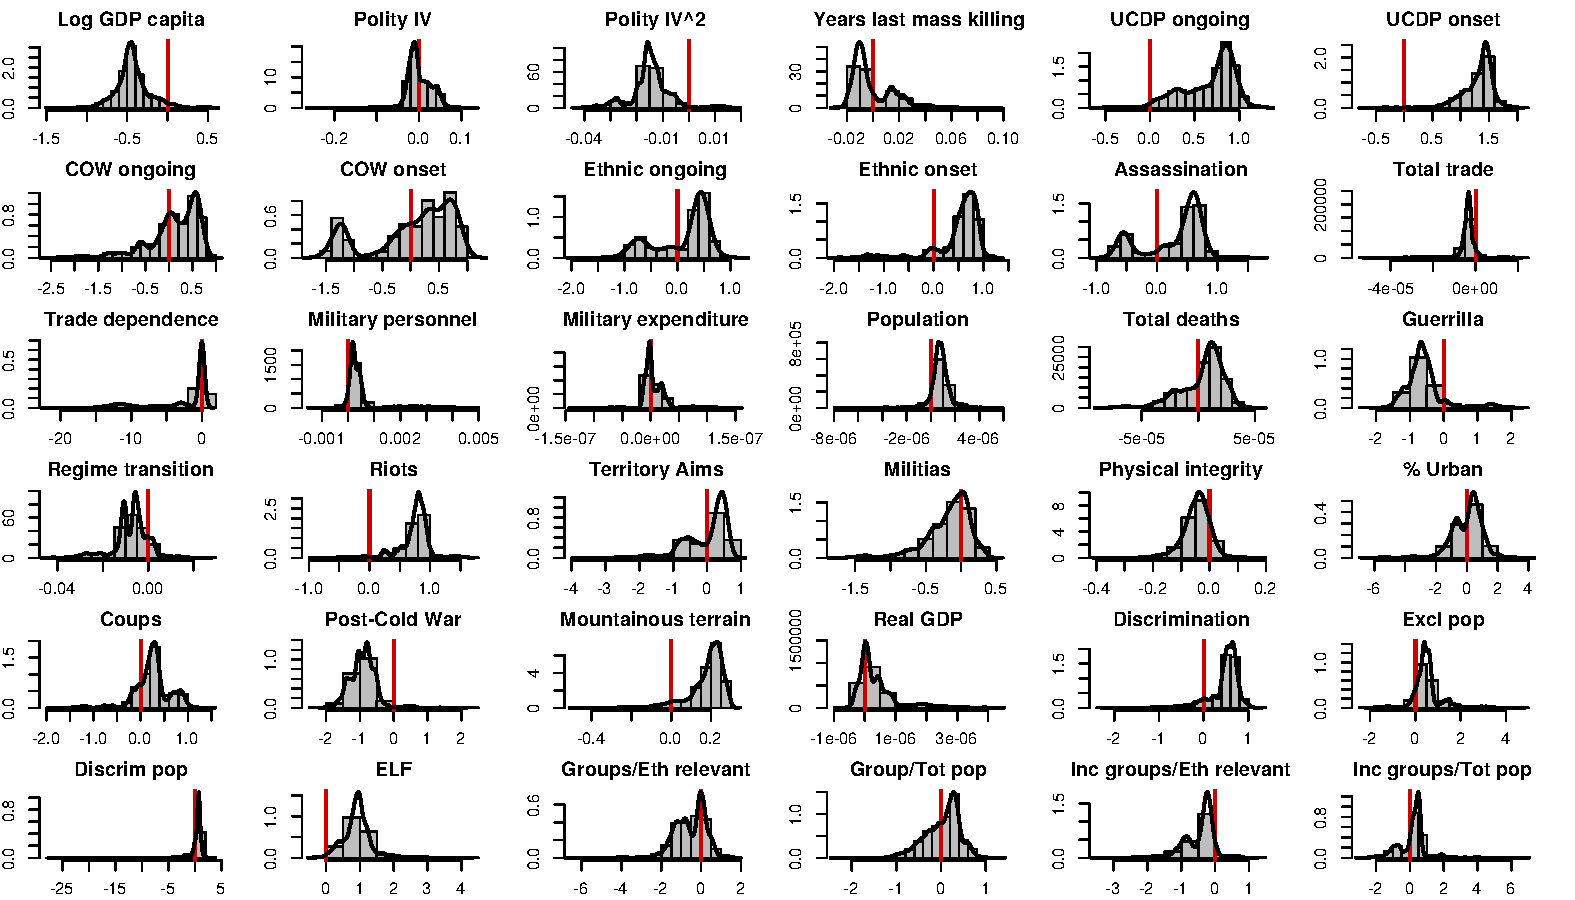
\includegraphics[width=.98\textheight,angle=90]{images/mk-logit.pdf}
    \caption{EBA -- Logistic Regression}
    \label{fig:mk-logit}
\end{figure}

\begin{table}[H]
\centering
\begin{tabular}{lrrrrr}
\hline
\textbf{Variable} & \textbf{Avg. $\beta$} & \textbf{Avg. SE} & \textbf{$\%$ Sig.} & \textbf{CDF(0)} & \textbf{Models} \\ \hline
\textit{Base variables} &  &  &  &  &  \\
Log GDP per capita & -0.1924 & 0.1031 & 76.118 & 0.9258 & 50000 \\
 &  &  &  &  &  \\
\textit{Additional variables} &  &  &  &  &  \\
UCDP civil war onset & 0.6422 & 0.2582 & 89.225 & 0.9772 & 4501 \\
Previous riots & 0.3367 & 0.1743 & 71.813 & 0.9436 & 7851 \\
Post-Cold War years & -0.3709 & 0.1830 & 71.465 & 0.9404 & 7836 \\
Polity IV squared & -0.0061 & 0.0032 & 70.155 & 0.9315 & 7931 \\ \hline
\end{tabular}
\caption{EBA -- Probit Regression}
\label{tab:eba1}
\end{table}

\begin{figure}
    \centering
    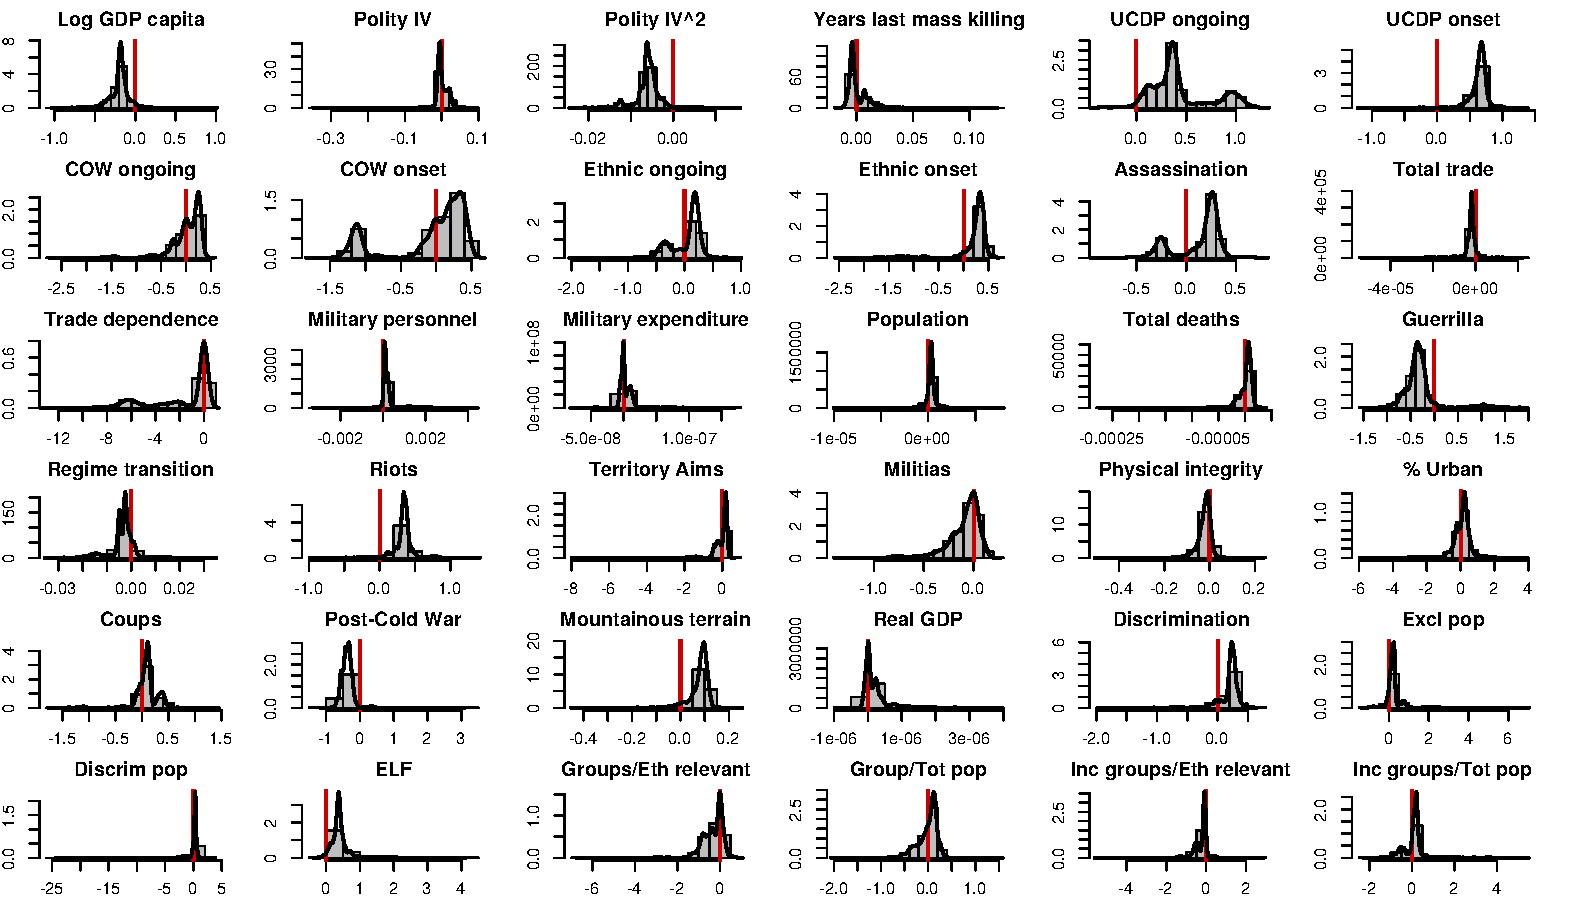
\includegraphics[width=.98\textheight,angle=90]{images/mk-probit.pdf}
    \caption{EBA -- Probit Regression}
    \label{fig:mk-probit}
\end{figure}

\subsection{Harff's Genocides and Politicides Data}
\label{sec:harff}

\subsubsection{Main Model}

In this section, we evaluate the models presented above with a measure of genocide and politicide by \citet{harff2003no}. The results show important contrasts with the previous analyses. First, no variable appear as significant in the main extreme bounds analysis. That is, none of the 36 predictors reached the threshold of CDF(0) $> 0.9$. Thus, we do not present a table with the results. The variable that came closest to significance was a dummy indicator of coups d'état, which has a CDF(0) of 0.897 and, as expected, is positively correlated with the onset of genocides. The distibution of the covariates' coefficients are available in figure \ref{fig:uamk}.

\newpage 

\begin{figure}
    \centering
    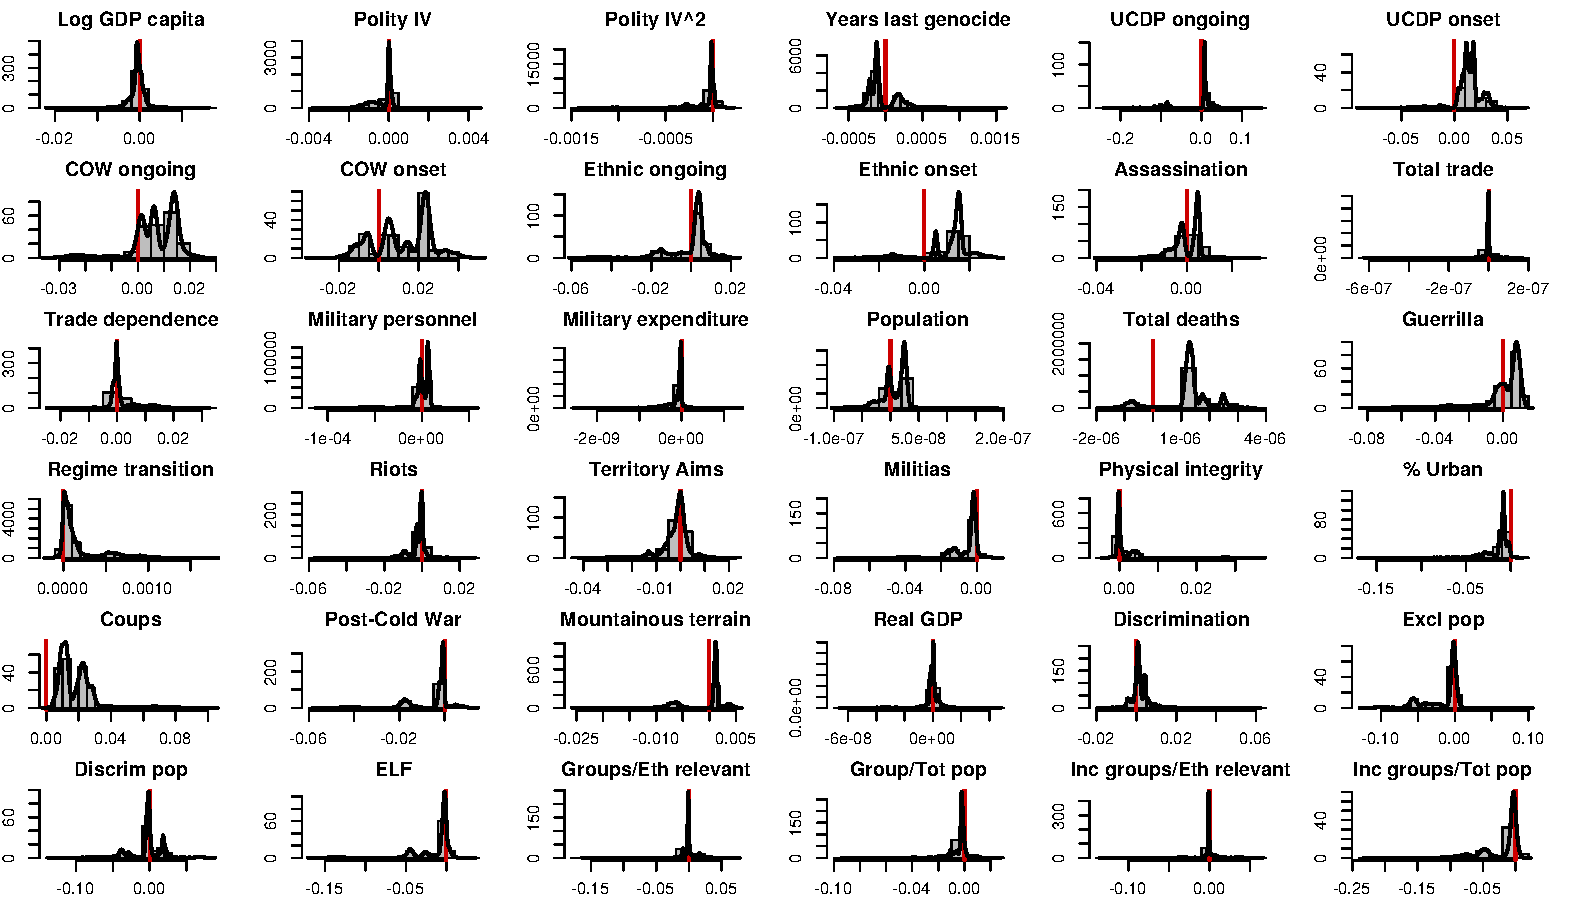
\includegraphics[width=.98\textheight,angle=90]{images/uamk.pdf}
    \caption{EBA -- Genocides and Politicides}
    \label{fig:uamk}
\end{figure}

\subsubsection{Genocides and Politicides during Civil Wars}

Next, we evaluate what covariates are robust when considering only genocides and politicide that occur during civil conflicts. Post-Cold War years again appear as a significant variable and with a negative sign; excluded population also has a negative impact on the outcome variable in two analyses.

\vspace{1cm}

\begin{table}[H]
\centering
\begin{tabular}{lrrrrr}
\hline
\textbf{Variable} & \textbf{Avg. $\beta$} & \textbf{Avg. SE} & \textbf{$\%$ Sig.} & \textbf{CDF(0)} & \textbf{Models} \\ \hline
\textit{UCDP data} &  &  &  &  &  \\
Excluded population & -0.037 & 0.022 & 64.524 & 0.9176 & 8758 \\
 &  &  &  &  &  \\
\textit{COW data} &  &  &  &  &  \\
Excluded population & -0.057 & 0.031 & 65.703 & 0.9570 & 8820 \\
Discriminated population & -0.050 & 0.029 & 53.850 & 0.9367 & 8767 \\
Post-Cold War years & -0.019 & 0.013 & 42.531 & 0.9203 & 8904 \\
 &  &  &  &  &  \\
\textit{Cederman et al. data} &  &  &  &  &  \\
Assassination dummy & -0.009 & 0.006 & 47.723 & 0.9232 & 8828 \\ \hline
\end{tabular}
\caption{EBA -- Genocides/Politicides}
\label{tab:uamk1}
\end{table}

\newpage
\begin{figure}
    \centering
    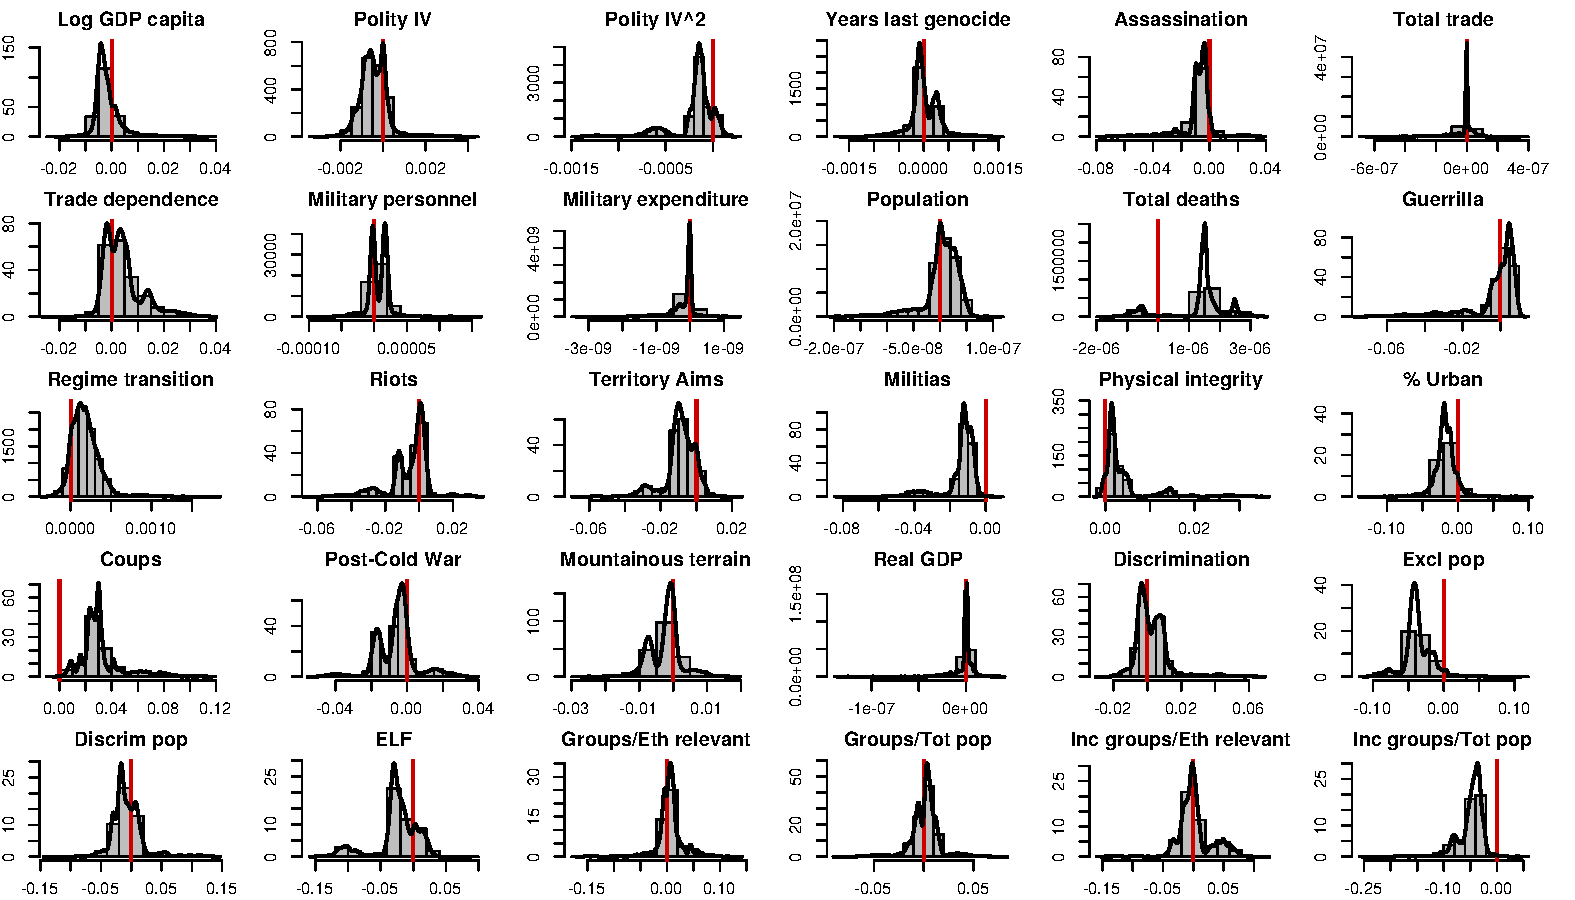
\includegraphics[width=.98\textheight, angle=90]{images/uamk-ucdp.pdf}
    \caption{EBA -- Genocides and Politicides during Civil Wars (UCDP Data)}
    \label{fig:uamk-ucdp}
\end{figure}

\begin{figure}
    \centering
    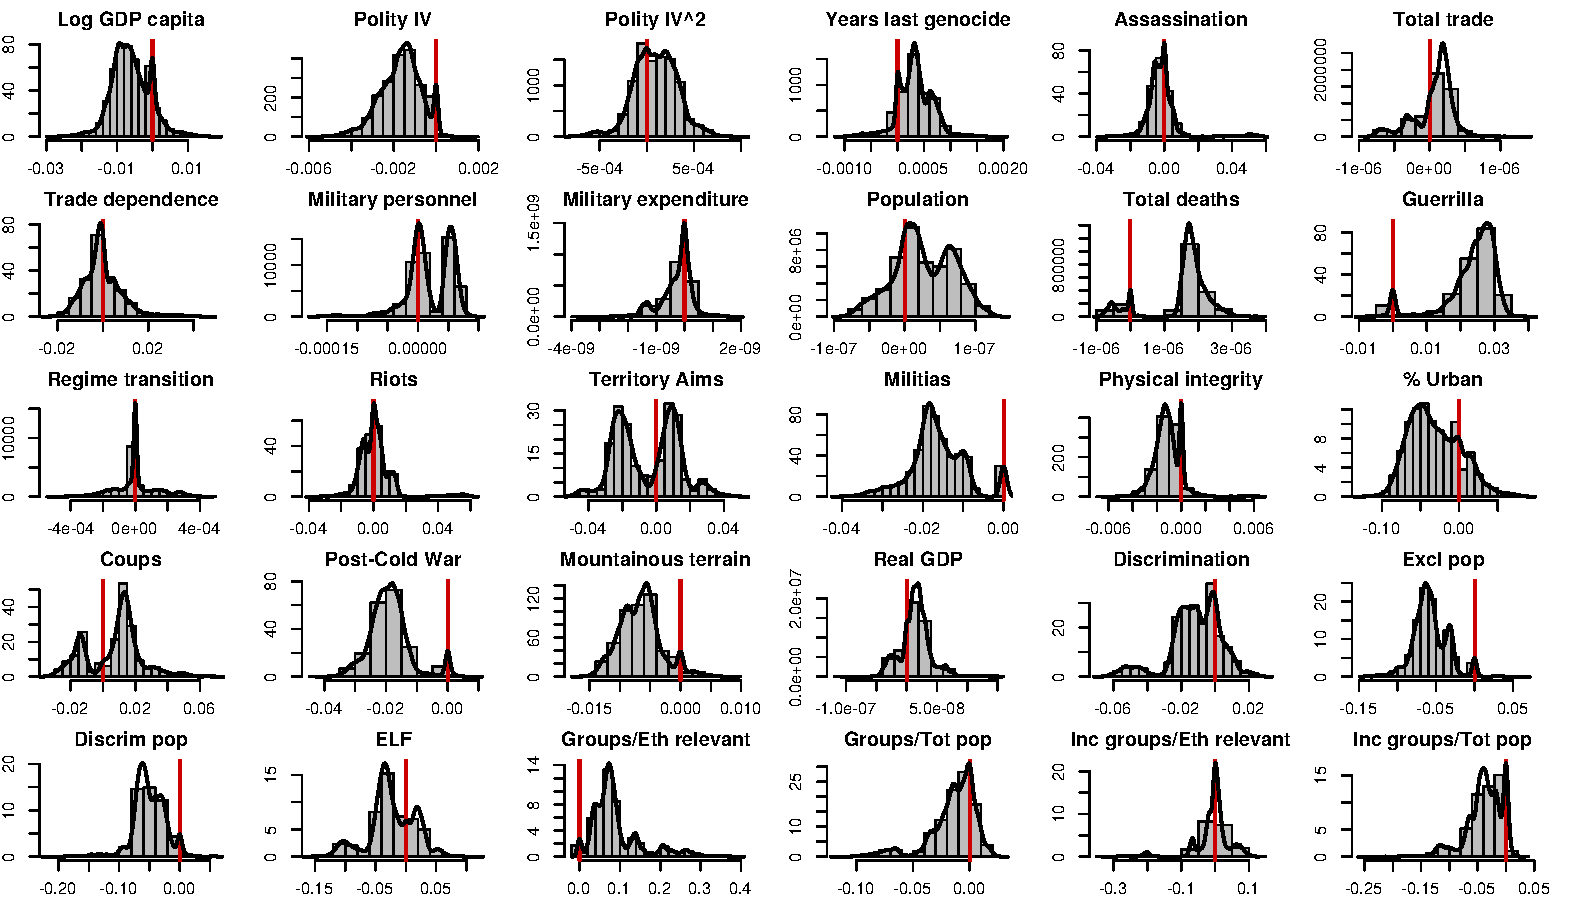
\includegraphics[width=.98\textheight, angle=90]{images/uamk-cow.pdf}
    \caption{EBA -- Genocides and Politicides during Civil Wars (COW Data)}
    \label{fig:uamk-cow}
\end{figure}

\begin{figure}
    \centering
    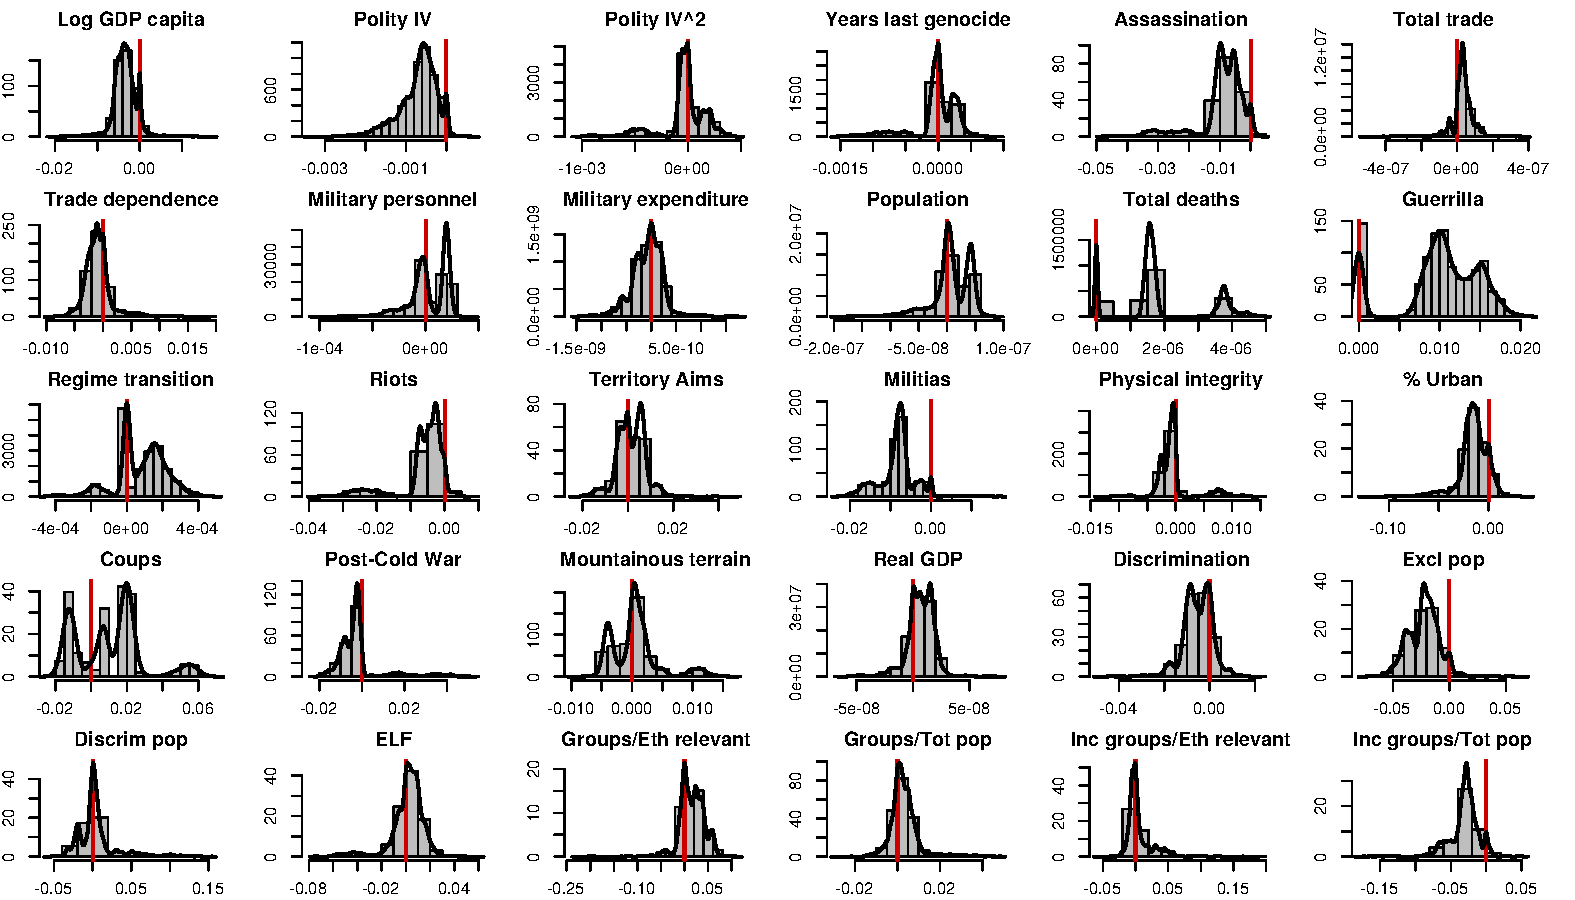
\includegraphics[width=.98\textheight, angle=90]{images/uamk-eth.pdf}
    \caption{EBA -- Genocides and Politicides during Ethnic Civil Wars (Cederman et al. Data)}
    \label{fig:uamk-eth}
\end{figure}

\newpage

\section{Random Forest}
\label{sec:mk-rfe}

\subsection{Main Model}

We employed the \texttt{H2O} machine learning platform \citep{h2o2017} to estimate the models. \texttt{H20} is open-source, optimised for big data and estimates a large number of models with only a few lines of code. We run the algorithms on 75\% of our dataset, and use the remaining 25\% as a validation set. That is, we use a percentage of the data to assess the main model's accuracy.\footnote{For more information about training and validation samples, please refer to \href{http://docs.h2o.ai/h2o/latest-stable/h2o-docs/data-science/algo-params/validation_frame.html}{\texttt{http://docs.h2o.ai/h2o/latest-stable/h2o-docs/data-science/algo-params/validation\_frame.html}}.} Our measure of accuracy is the area under the curve (AUC). All models score well in that regard, and measures of about 0.8 accuracy in our validation sample are common.

The next two plots show the results of the main random forest models. 

\begin{figure}[H]
    \centering
    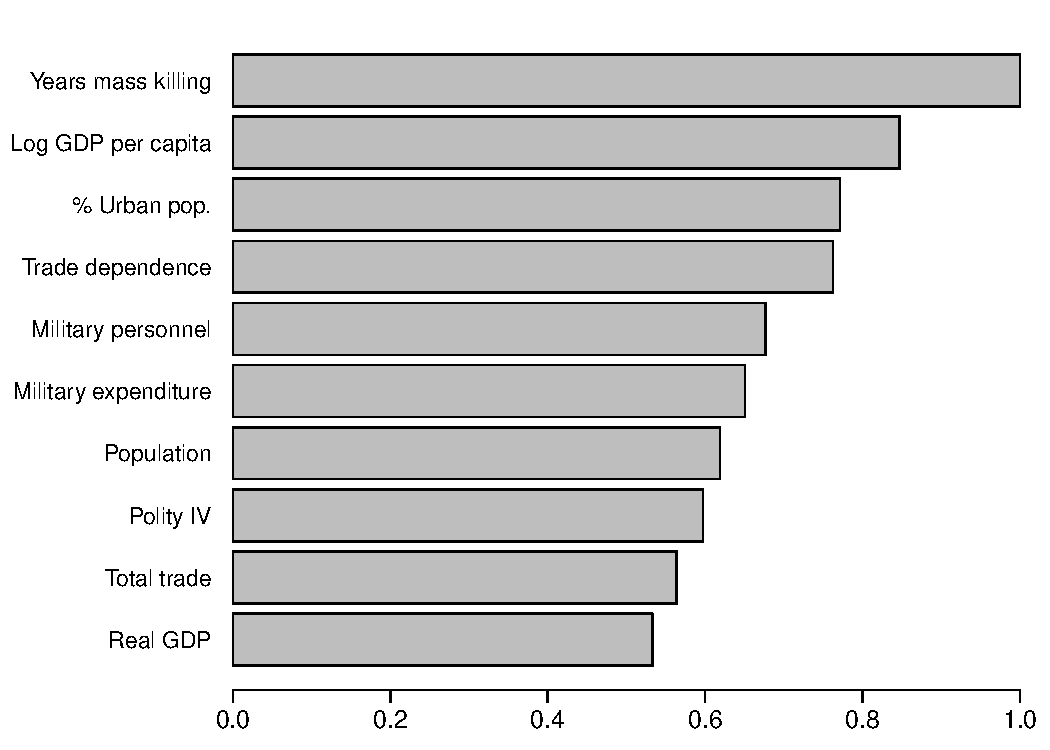
\includegraphics{images/rf-mk.pdf}
    \caption{Variable Importance -- Main Model}
    \label{fig:rf-mk}
\end{figure}

\newpage 

\begin{figure}[H]
    \centering
    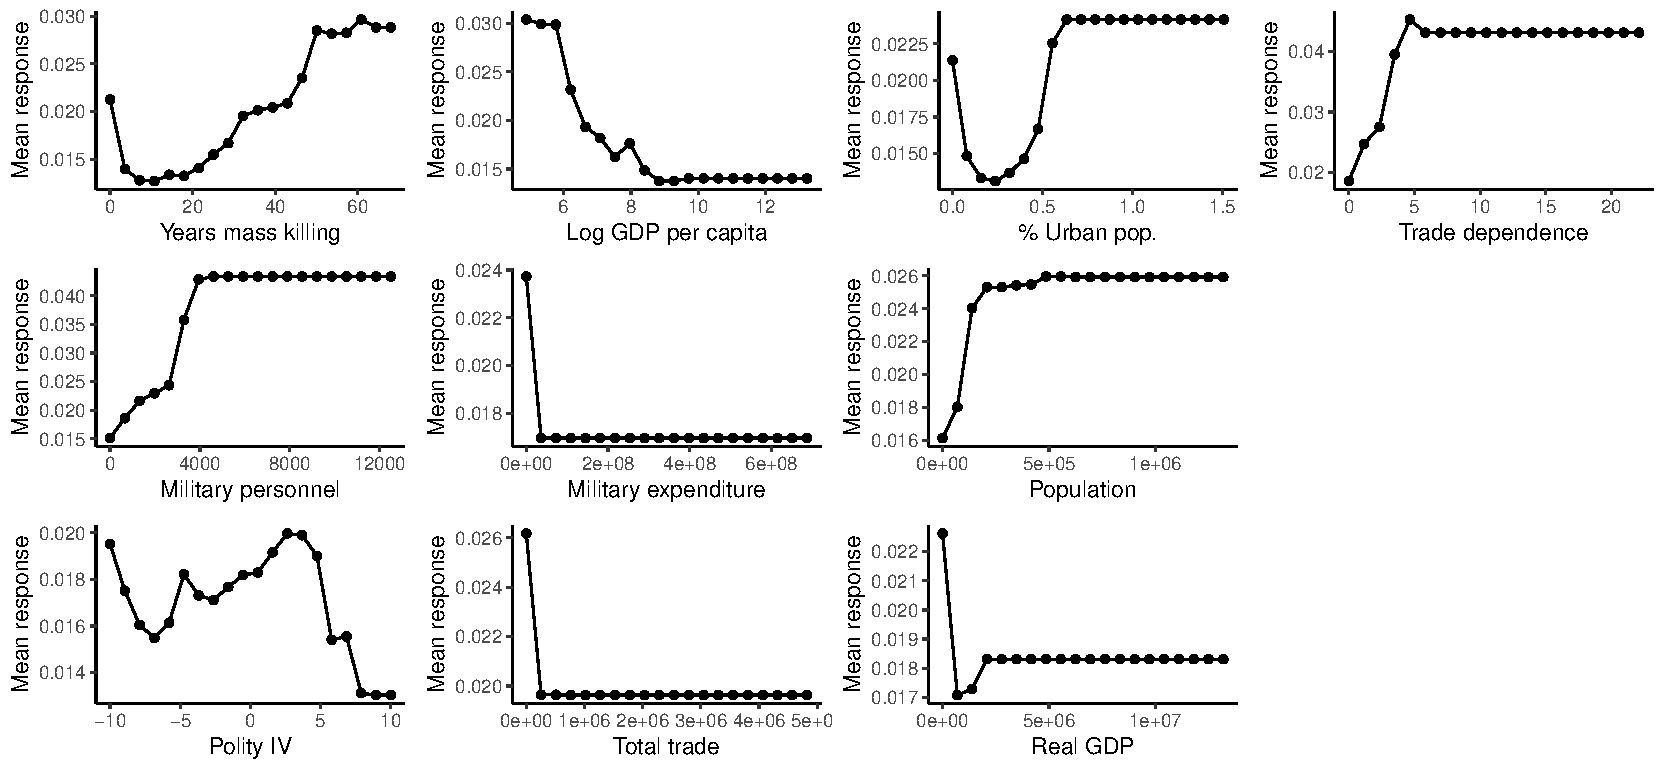
\includegraphics[width=.98\textheight,angle=90]{images/rf-mk-pd.pdf}
    \caption{Partial Dependence Plot -- Main Model}
    \label{fig:rf-mk-pd}
\end{figure}

\subsection{Genocides During Civil Wars}

The following graphs display the most important predictors of mass killings when we restrict our sample to cases that occur during civil wars. As we note in section \ref{sec:civil-wars}, we employ three different measures of civil conflicts. The first one is provided by the Uppsala Conflict Data Program \citep{allansson2017organized,gleditsch2002armed}, the second is offered by the Correlates of War \citep{sarkees2010resort}, and a third indicating the onset of ethnic conflict as coded by \citet{cederman2010ethnic}.  

\begin{figure}[H]
    \centering
    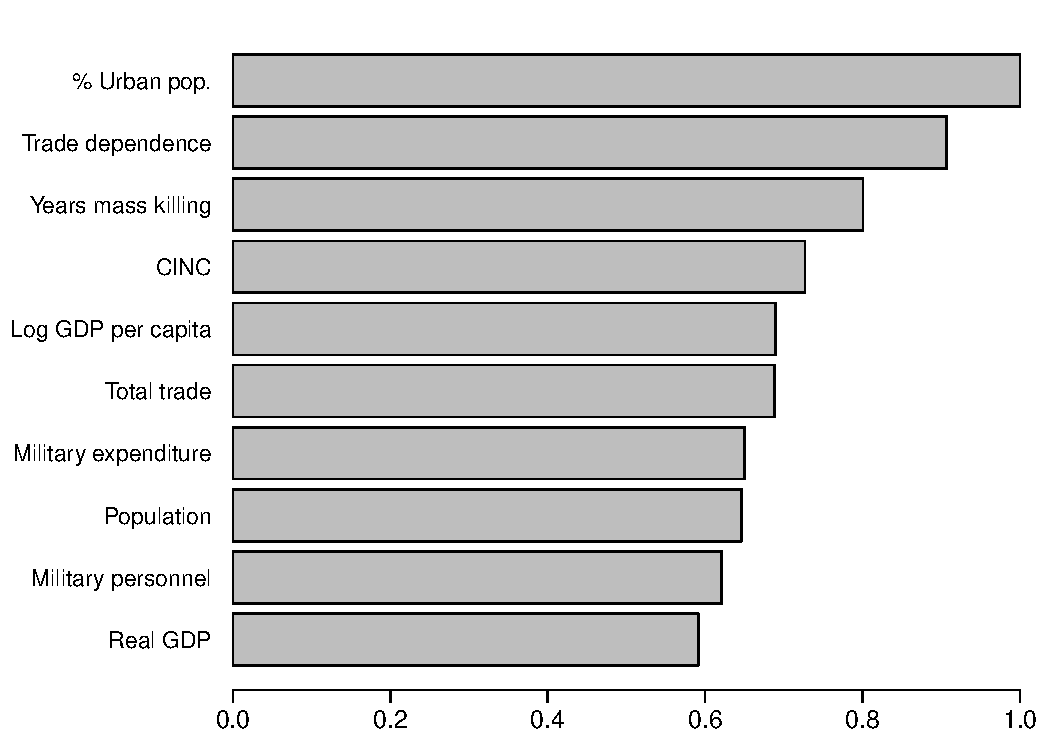
\includegraphics{images/rf-ucdp.pdf}
    \caption{Variable Importance -- Mass Killings during Civil Wars (UCDP Data)}
    \label{fig:rf-mk-ucdp}
\end{figure}

\newpage 

\begin{figure}[H]
    \centering
    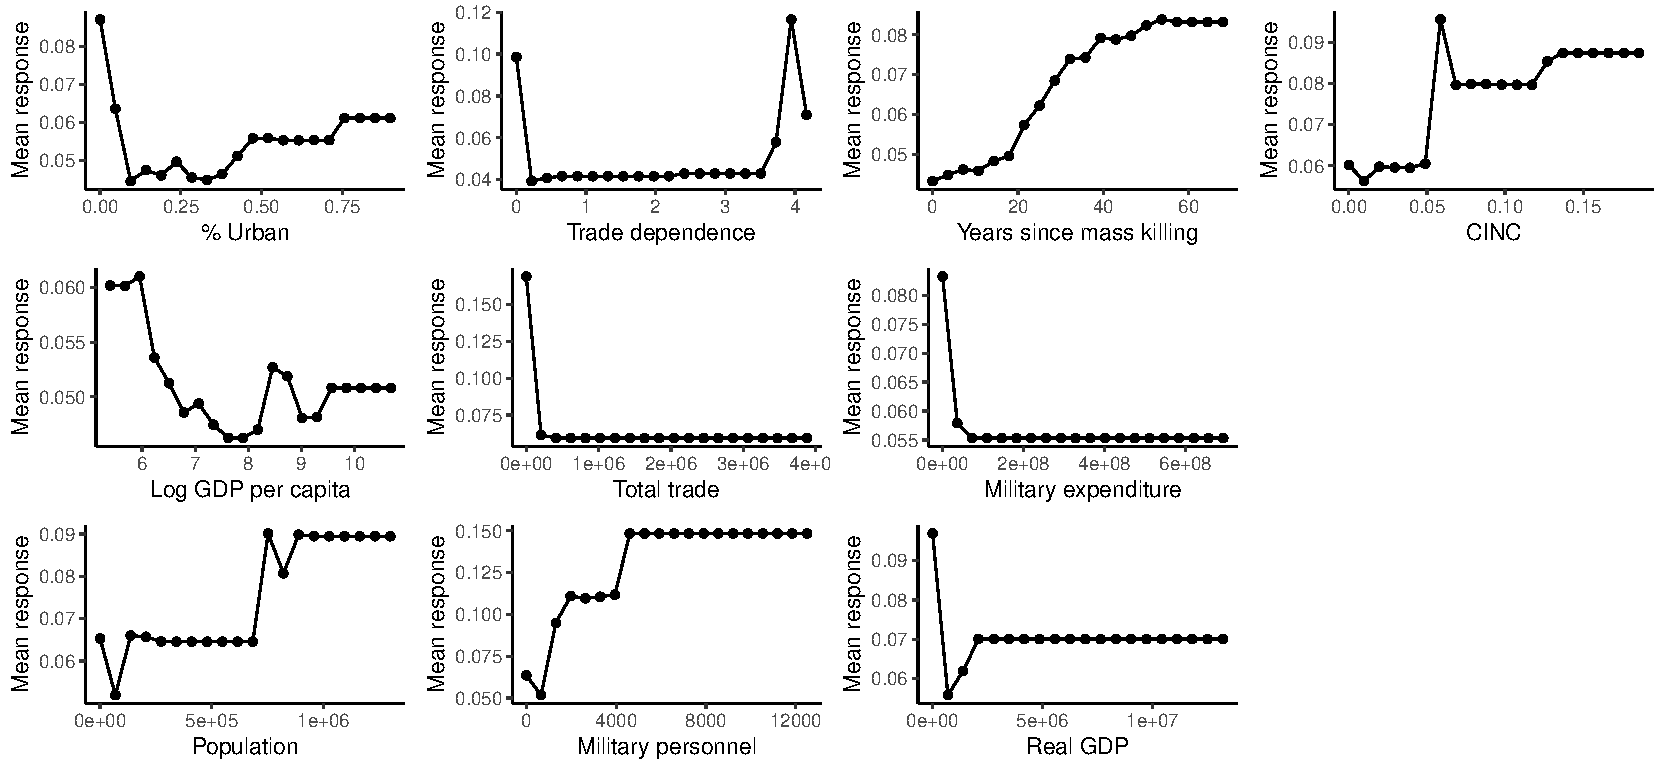
\includegraphics[width=.98\textheight,angle=90]{images/rf-ucdp-pd.pdf}
    \caption{Partial Dependence Plot -- Mass Killings during Civil Wars (UCDP Data)}
    \label{fig:rf-mk-ucdp-pd}
\end{figure}

\begin{figure}[H]
    \centering
    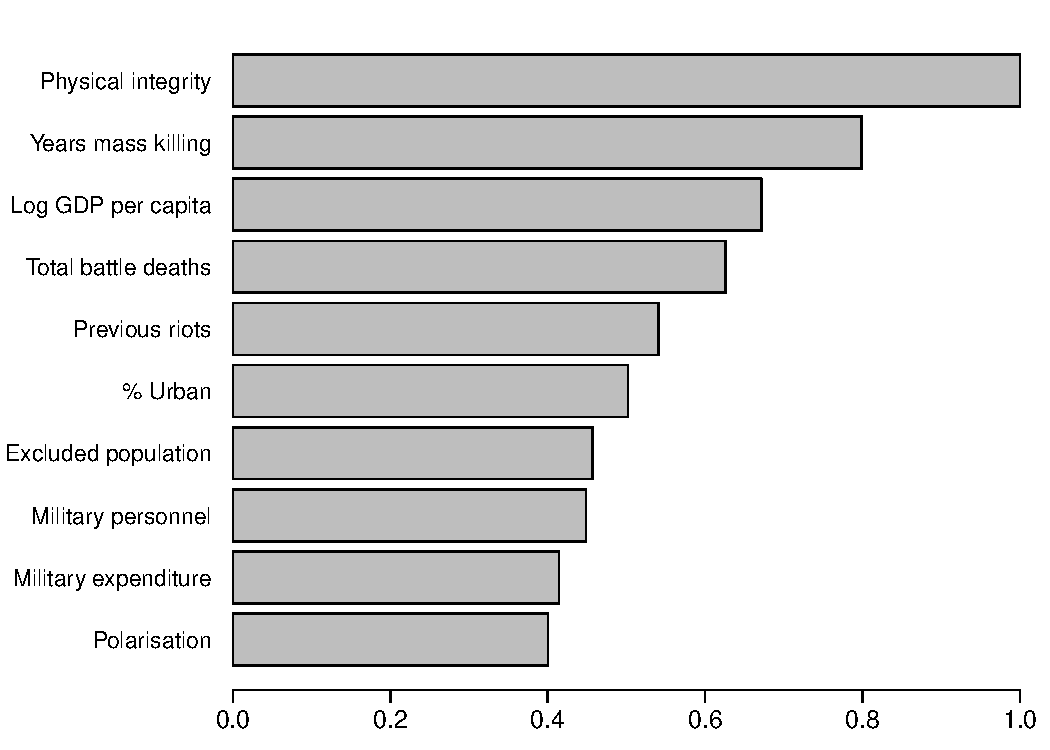
\includegraphics{images/rf-cow.pdf}
    \caption{Variable Importance -- Mass Killings during Civil Wars (COW Data)}
    \label{fig:rf-mk-ucdp}
\end{figure}

\newpage 

\begin{figure}[H]
    \centering
    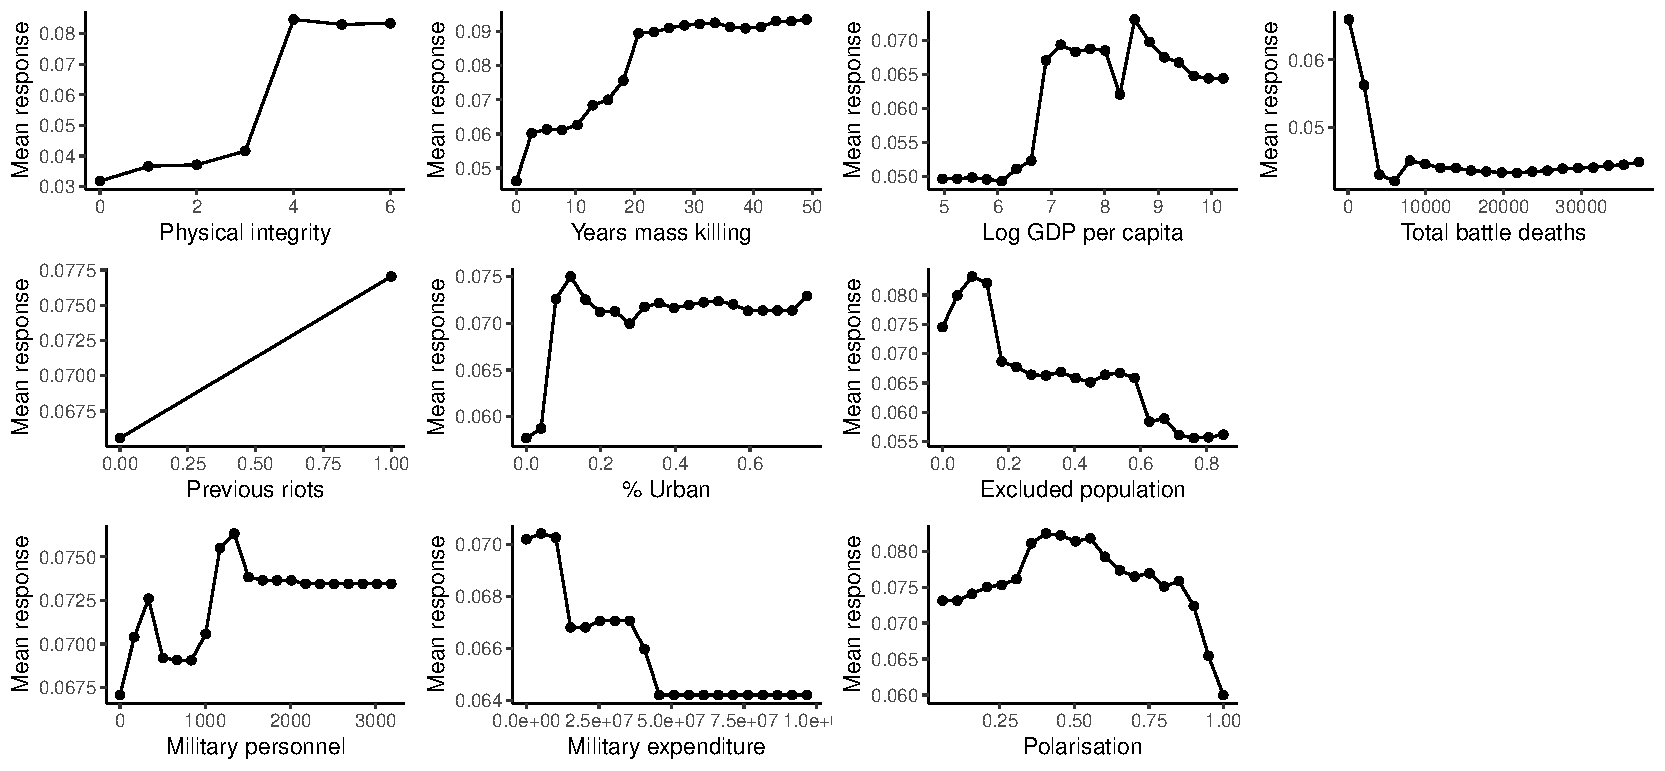
\includegraphics[width=.98\textheight,angle=90]{images/rf-cow-pd.pdf}
    \caption{Partial Dependence Plot -- Mass Killings during Civil Wars (COW Data)}
    \label{fig:rf-mk-ucdp-pd}
\end{figure}

\begin{figure}[H]
    \centering
    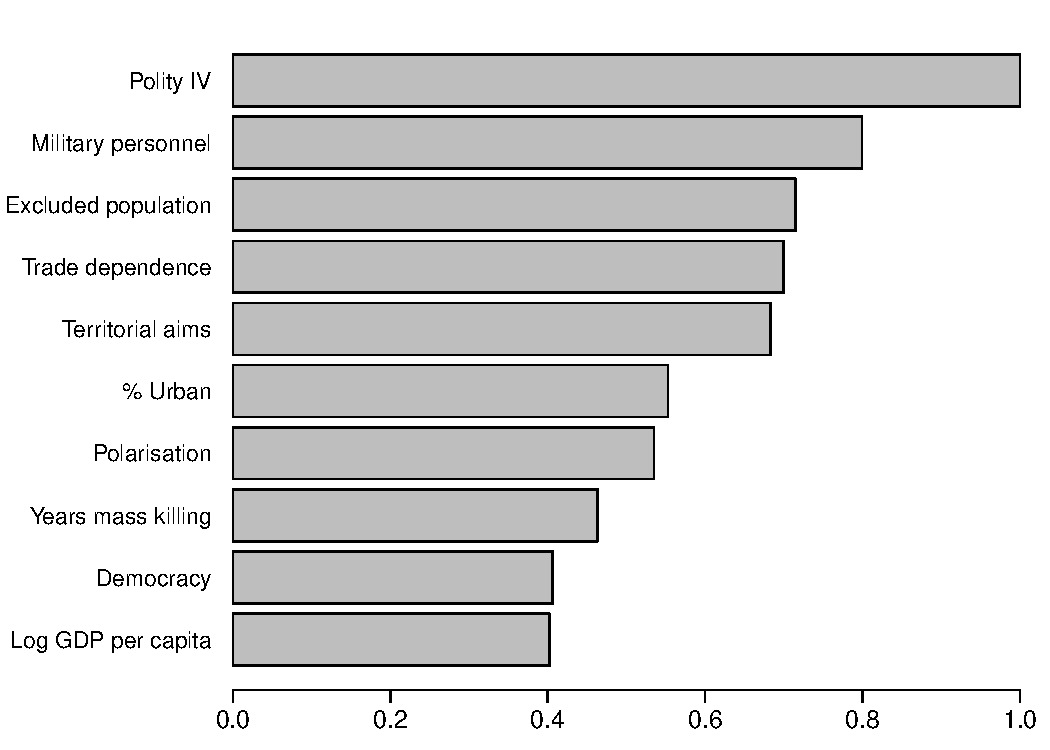
\includegraphics{images/rf-eth.pdf}
    \caption{Variable Importance -- Mass Killings during Civil Wars (Cederman et al. Data)}
    \label{fig:rf-mk-ucdp}
\end{figure}

\newpage 

\begin{figure}[H]
    \centering
    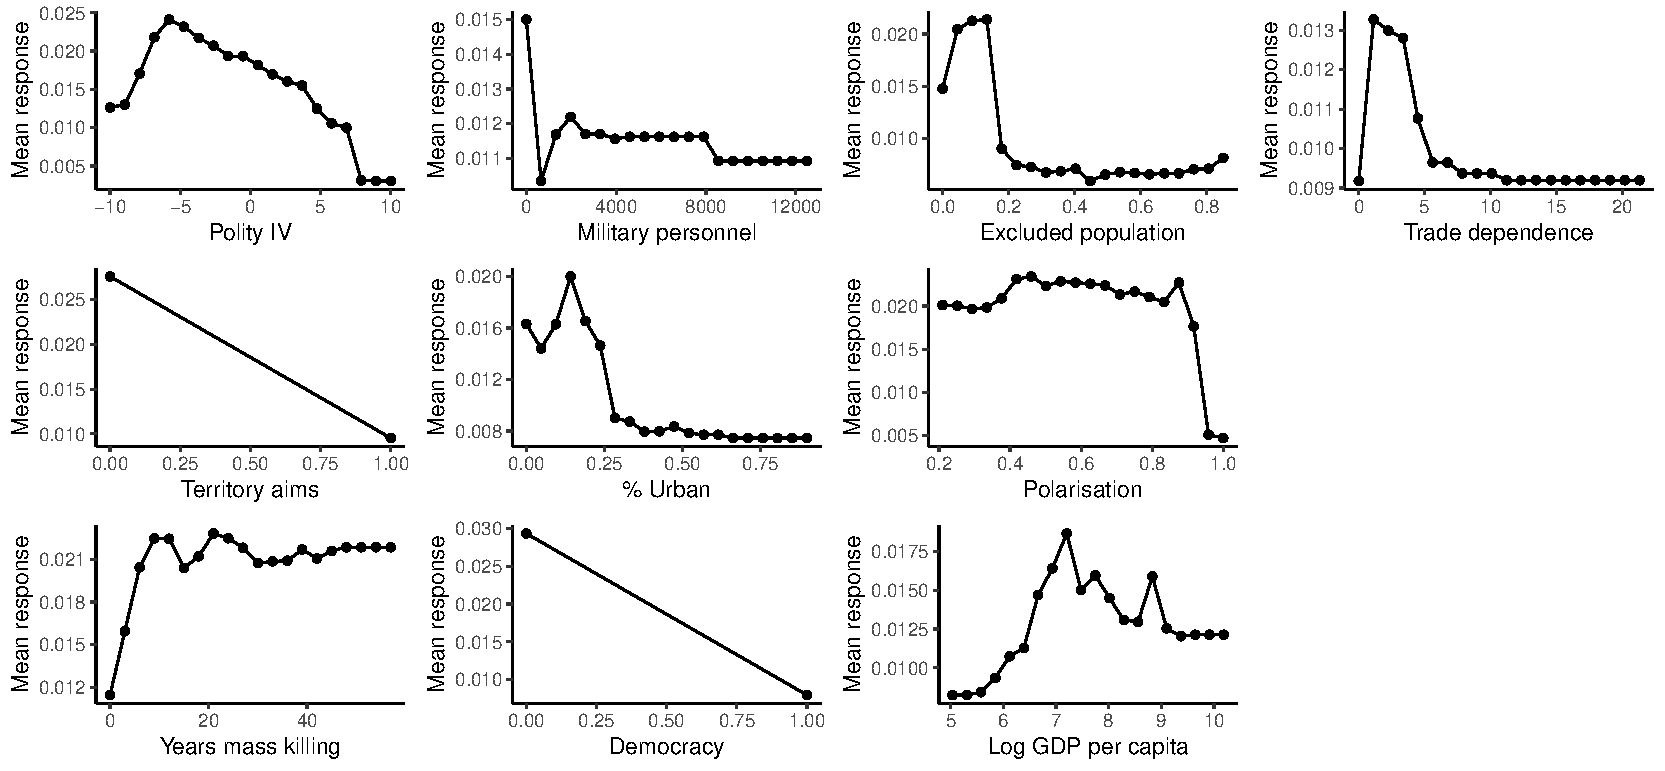
\includegraphics[width=.98\textheight,angle=90]{images/rf-eth-pd.pdf}
    \caption{Partial Dependence Plot -- Mass Killings during Civil Wars (Cederman et al. Data)}
    \label{fig:rf-mk-ucdp-pd}
\end{figure}

\newpage

\subsection{Alternative Random Seeds}

As random forests themselves are an approximation to a number of possible parameter combinations, changes in seed numbers may influence the model output. Thus, we start the main model with two different random seed numbers to check if the results are robust.\footnote{The numbers were generated at \href{https://www.random.org/}{\texttt{https://www.random.org/}}.} The main findings hold well; although variable importance changes from one model to another, the most significant variables appear repeatedly in the estimations. The marginal plots also show that the effect of the independent variables remain roughly similar despite the nonlinearities. The graphs below display the ten most significant predictors of mass killings and their respective partial dependence plots.

\begin{figure}[H]
    \centering
    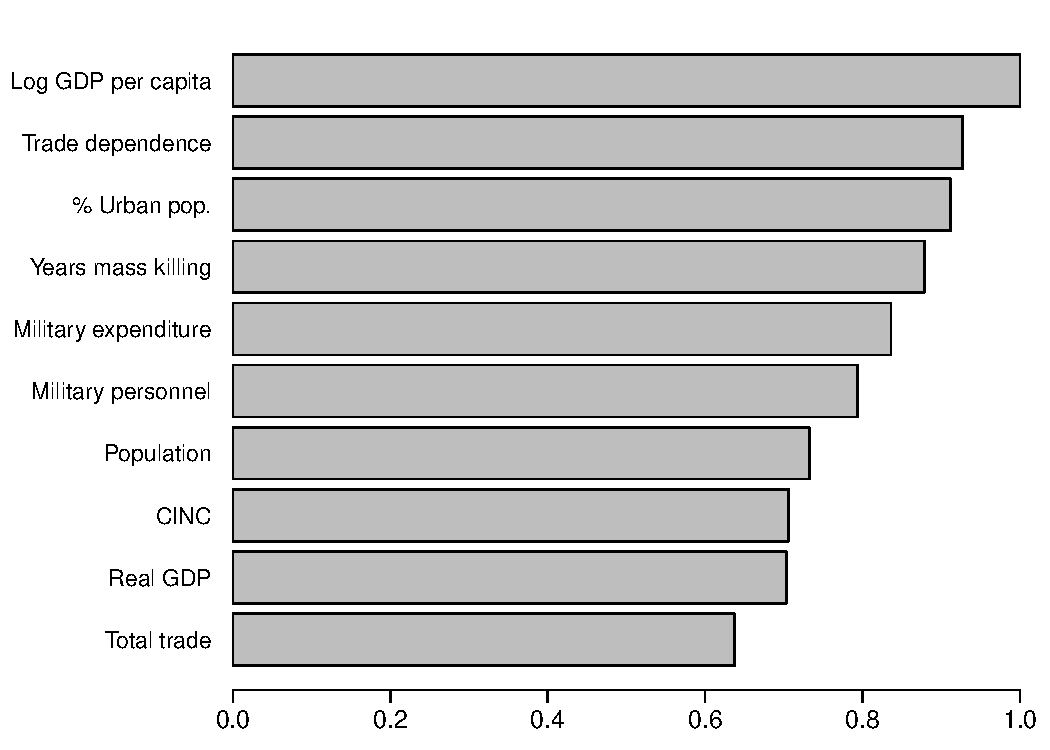
\includegraphics{images/rf-mk-4363.pdf}
    \caption{Variable Importance -- Seed 4363}
    \label{fig:rf-mk-4363}
\end{figure}

\newpage

\begin{figure}[H]
    \centering
    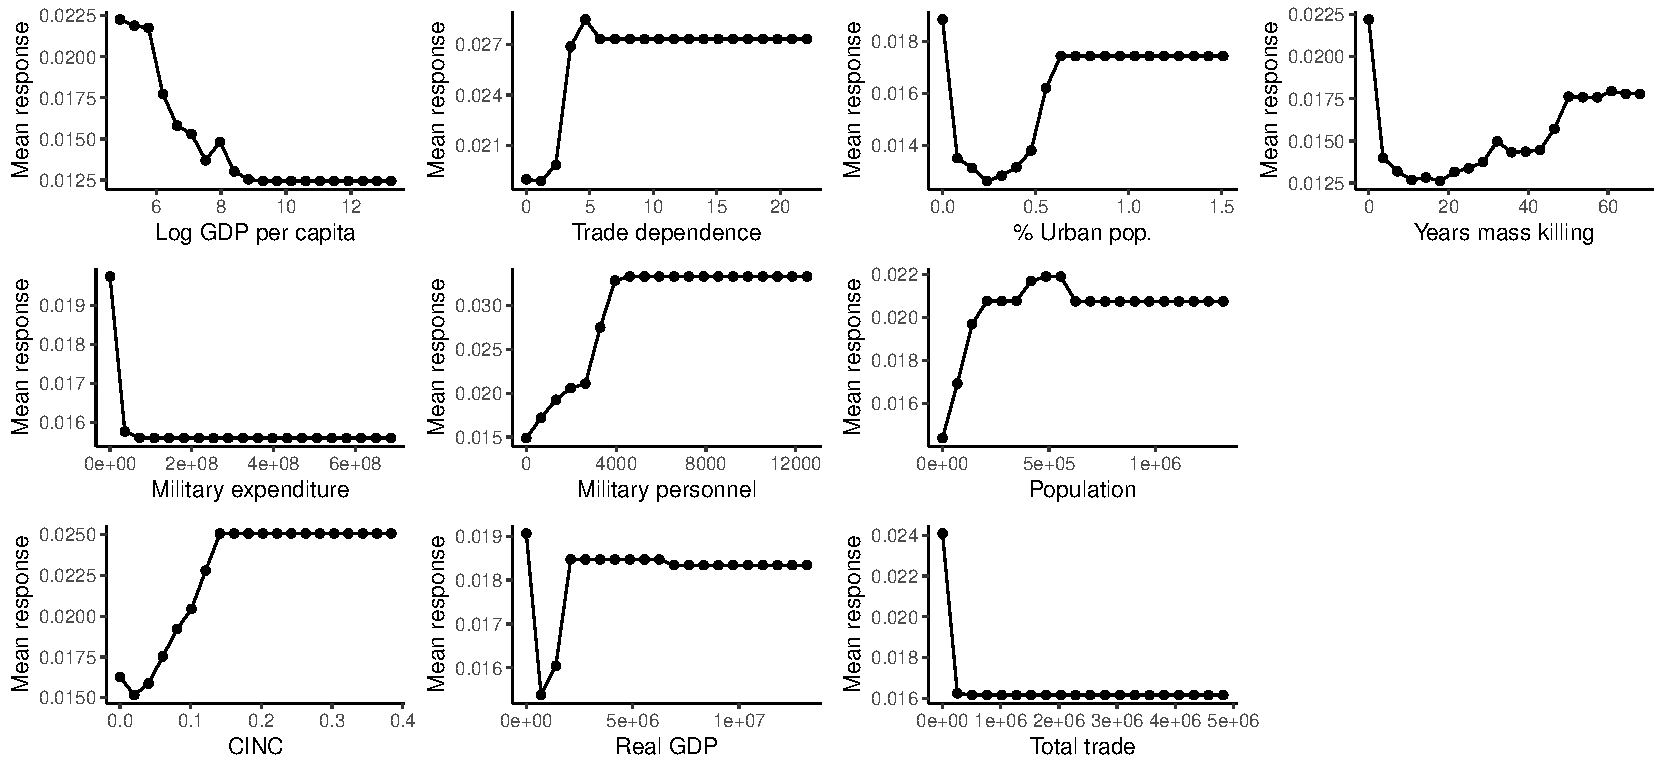
\includegraphics[width=.98\textheight,angle=90]{images/rf-mk-4363-pd.pdf}
    \caption{Partial Dependence Plot -- Seed 4363}
    \label{fig:rf-mk-4363}
\end{figure}

\newpage

\begin{figure}[H]
    \centering
    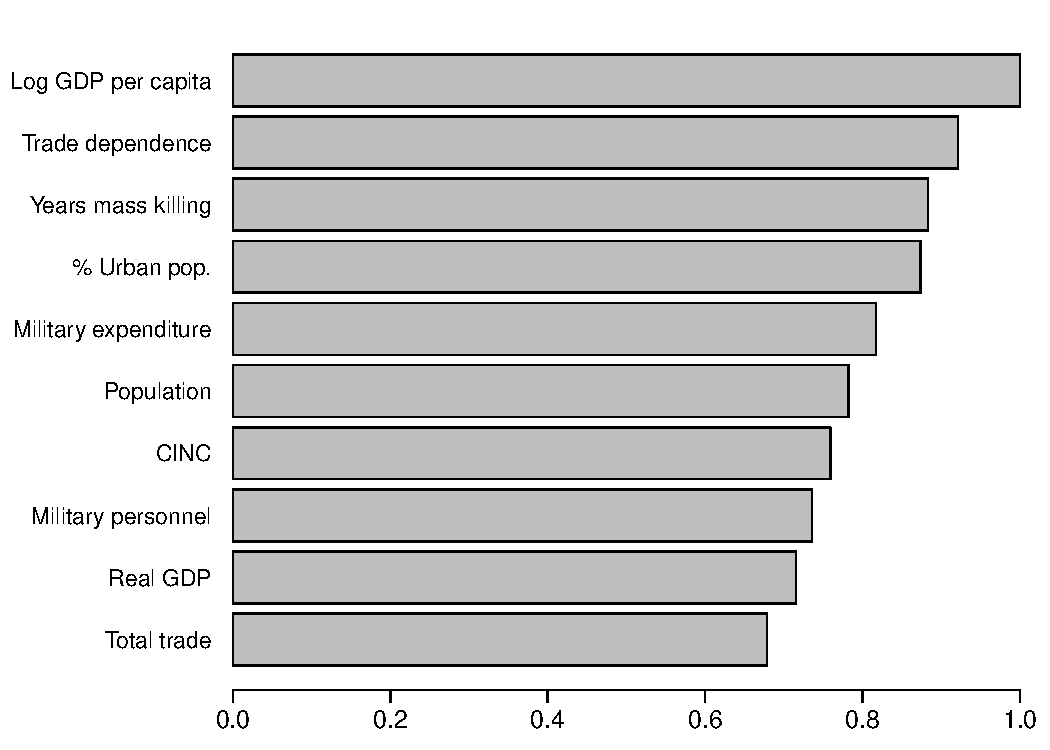
\includegraphics{images/rf-mk-7015.pdf}
    \caption{Variable Importance -- Seed 7015}
    \label{fig:rf-mk-4363}
\end{figure}

\newpage

\begin{figure}[H]
    \centering
    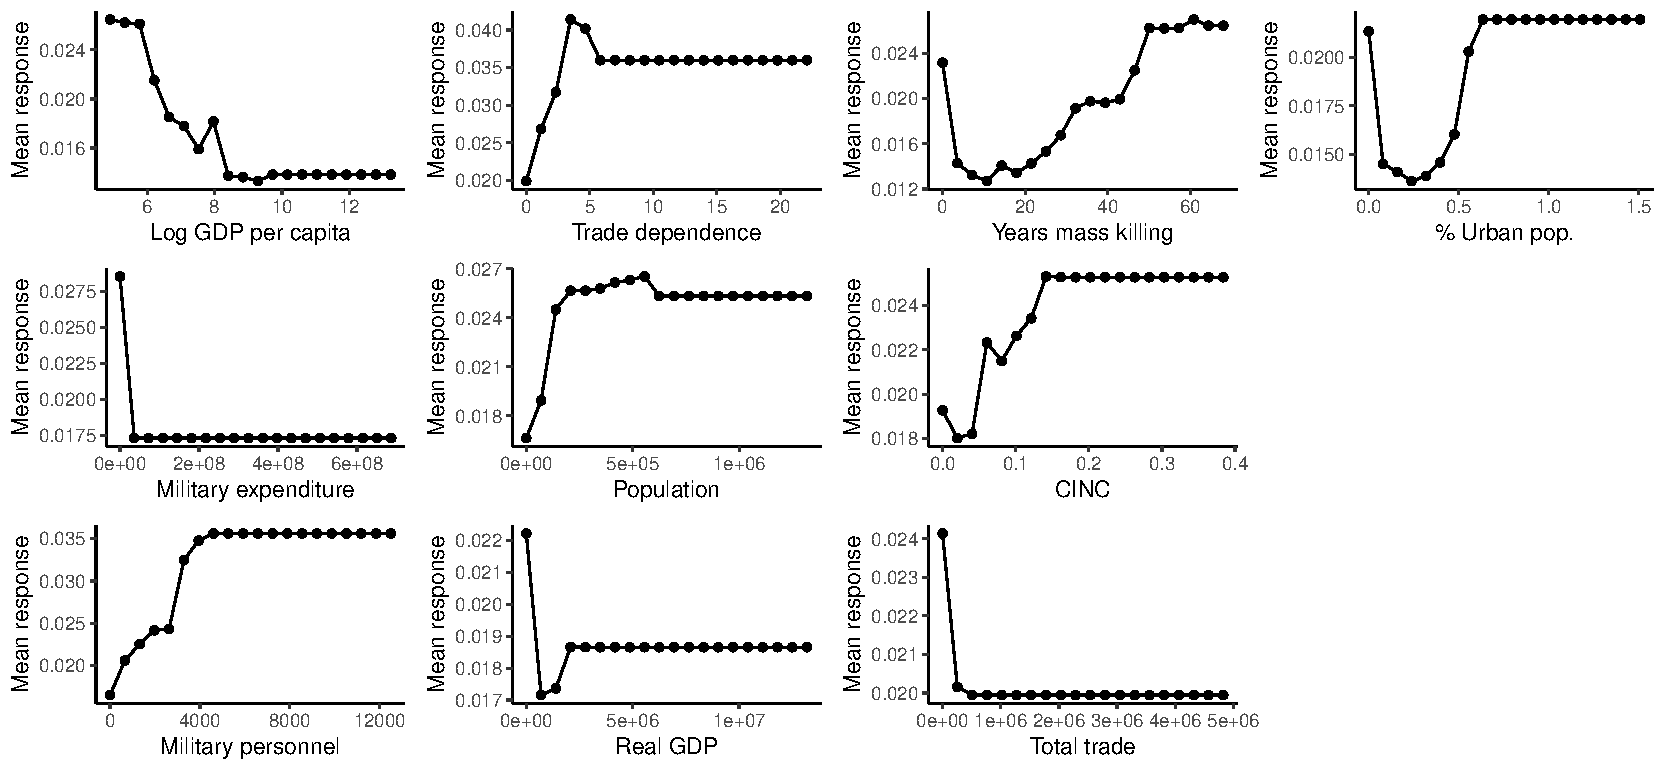
\includegraphics[width=.98\textheight,angle=90]{images/rf-mk-7015-pd.pdf}
    \caption{Partial Dependence Plot -- Seed 7015}
    \label{fig:rf-mk-4363}
\end{figure}

\newpage

\subsection{Harff's Genocides and Politicides Data}

\subsubsection{Main Model}

We replicate the same analysis using Harff's \citeyear{harff2003no} data. The results are comparable to the ones presented above. A similar set of variables appear in this model.

\begin{figure}[H]
    \centering
    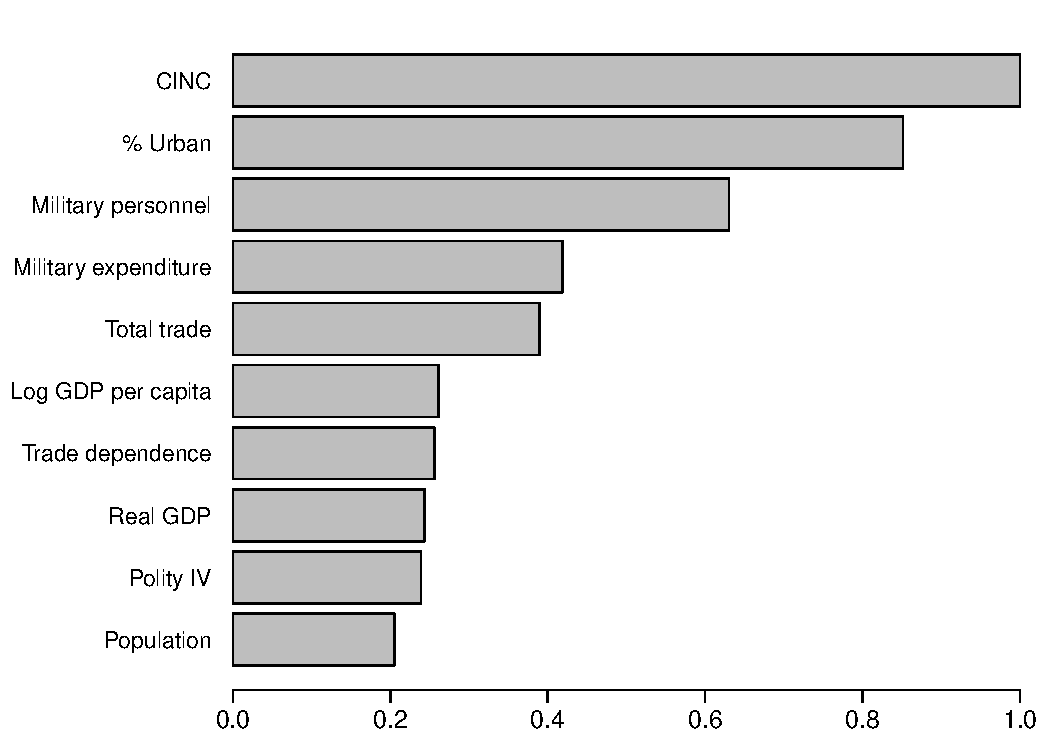
\includegraphics{images/rf-uamk.pdf}
    \caption{Variable Importance -- Genocides and Politicides}
    \label{fig:rf-mk-4363}
\end{figure}

\newpage

\begin{figure}[H]
    \centering
    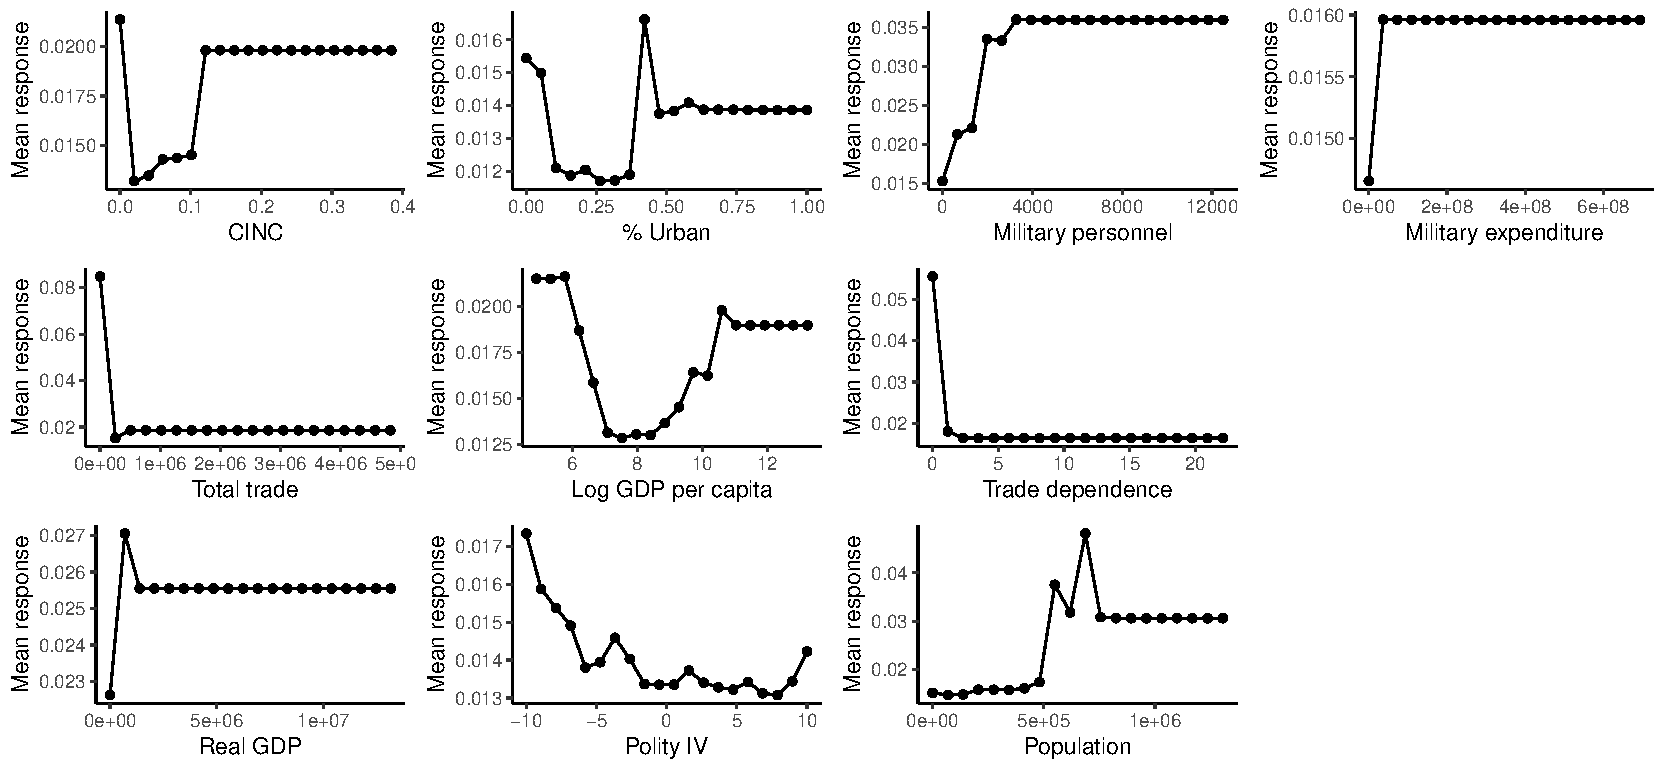
\includegraphics[width=.98\textheight,angle=90]{images/rf-uamk-pd.pdf}
    \caption{Partial Dependence Plot -- Genocides and Politicides}
    \label{fig:rf-mk-4363}
\end{figure}

\newpage

\subsubsection{Genocides and Politicides during Civil Wars}

Lastly, the graphs below show the results of the grid search when we only include civil war years. 

\begin{figure}[H]
    \centering
    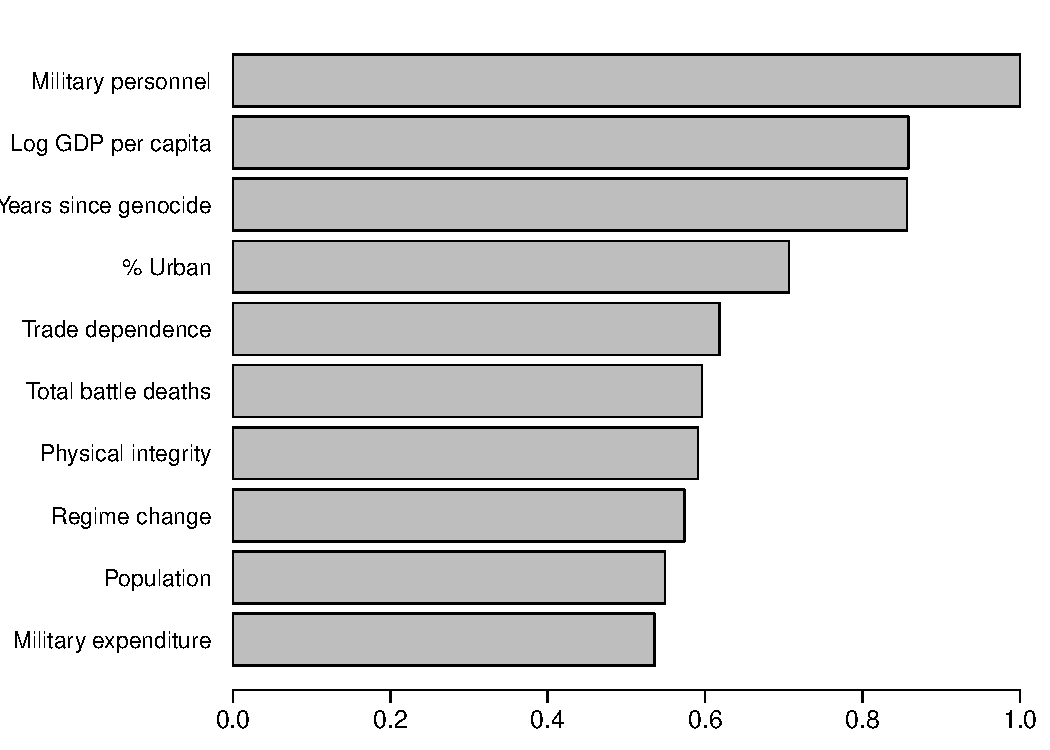
\includegraphics{images/rf-uamk-ucdp.pdf}
    \caption{Variable Importance -- Genocides and Politicides during Civil Wars (UCDP Data)}
    \label{fig:rf-mk-ucdp}
\end{figure}

\newpage 

\begin{figure}[H]
    \centering
    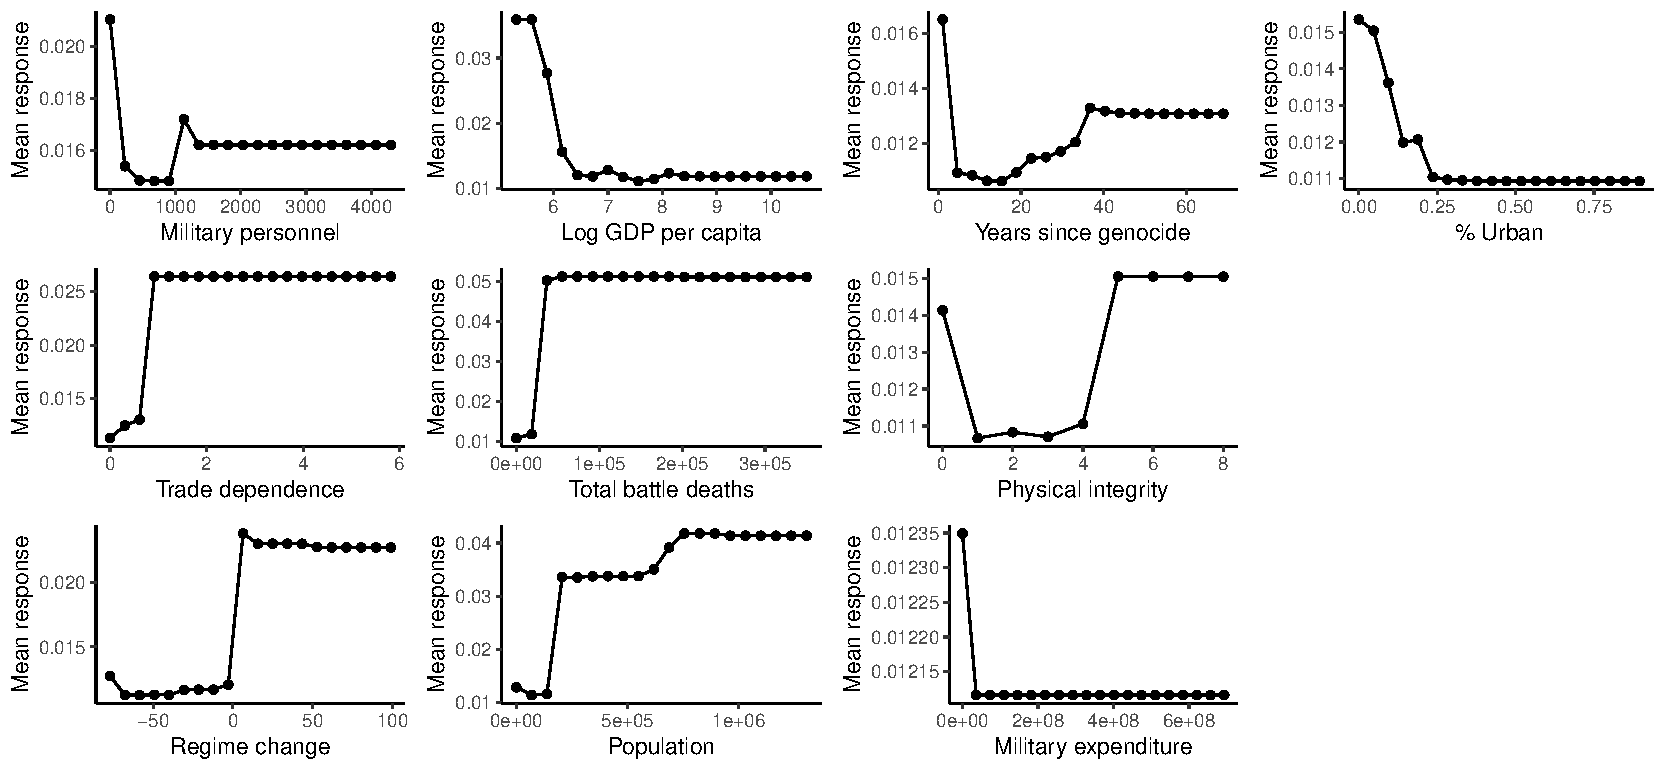
\includegraphics[width=.98\textheight,angle=90]{images/rf-uamk-ucdp-pd.pdf}
    \caption{Partial Dependence Plot -- Genocides and Politicides during Civil Wars (UCDP Data)}
    \label{fig:rf-mk-ucdp-pd}
\end{figure}

\begin{figure}[H]
    \centering
    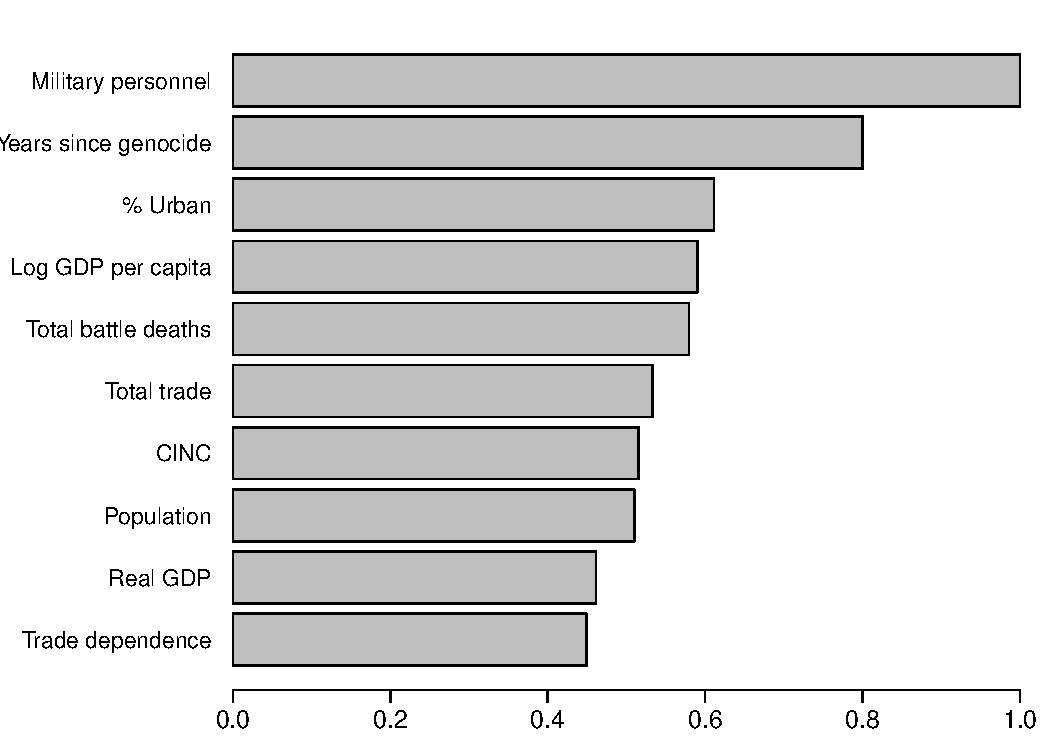
\includegraphics{images/rf-uamk-cow.pdf}
    \caption{Variable Importance -- Genocides and Politicides during Civil Wars (COW Data)}
    \label{fig:rf-mk-ucdp}
\end{figure}

\newpage 

\begin{figure}[H]
    \centering
    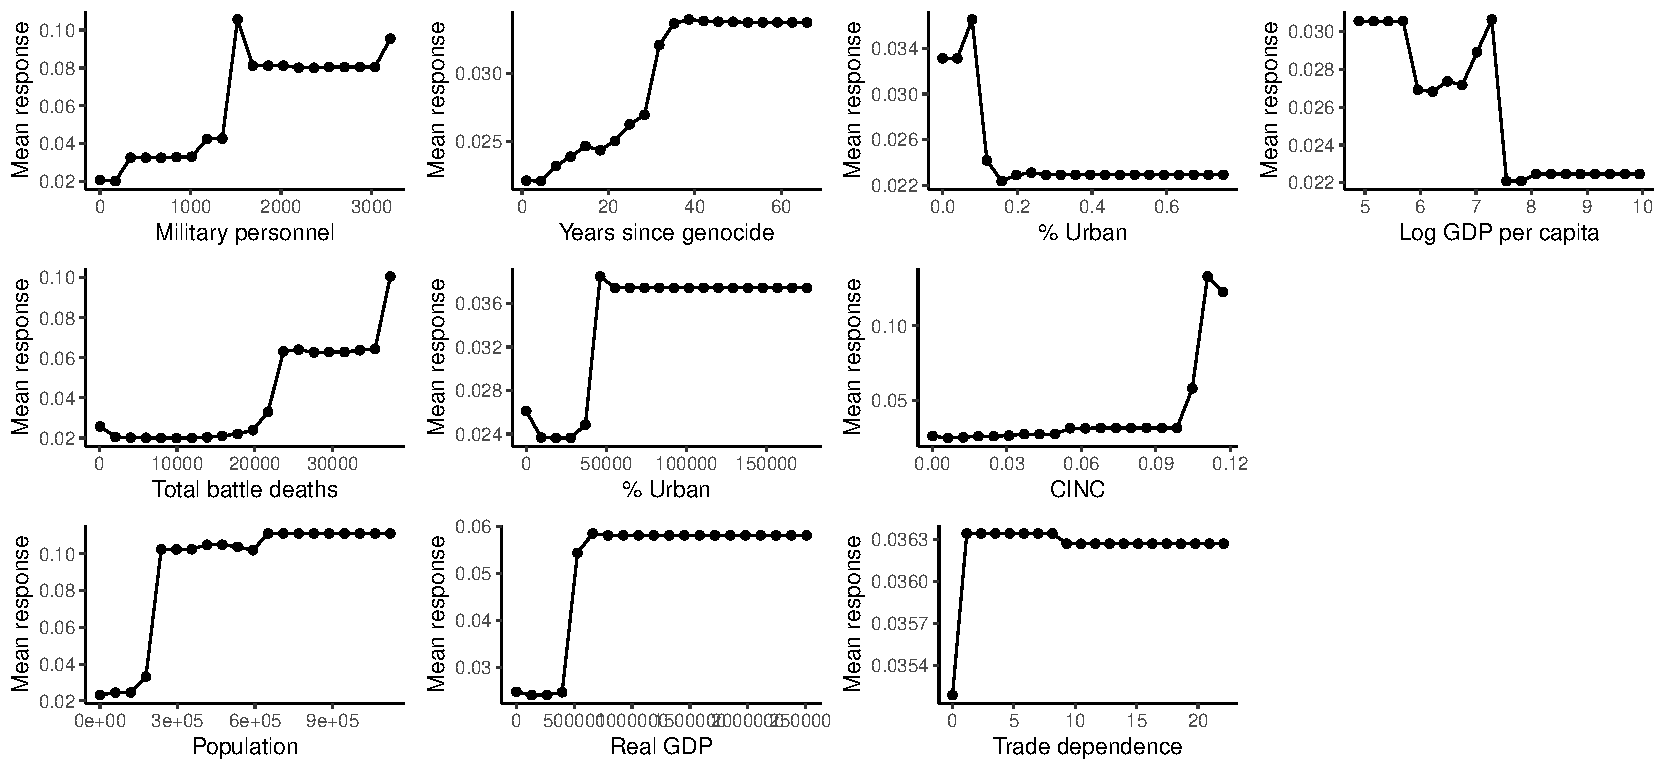
\includegraphics[width=.98\textheight,angle=90]{images/rf-uamk-cow-pd.pdf}
    \caption{Partial Dependence Plot -- Genocides and Politicides during Civil Wars (COW Data)}
    \label{fig:rf-mk-ucdp-pd}
\end{figure}

\begin{figure}[H]
    \centering
    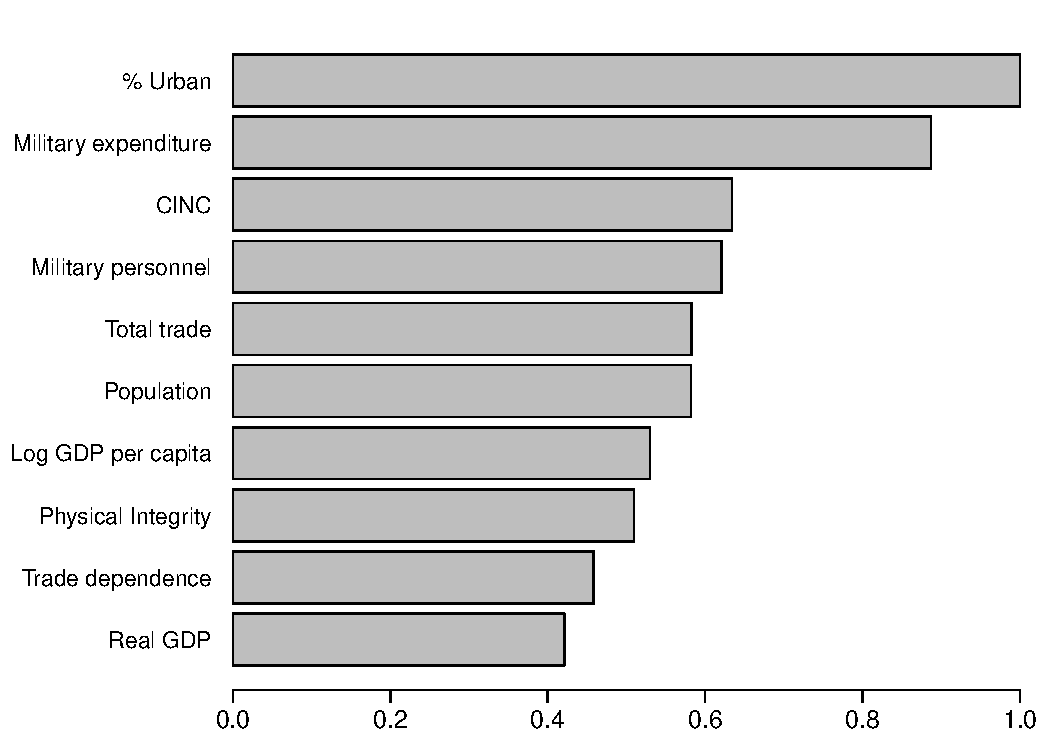
\includegraphics{images/rf-uamk-eth.pdf}
    \caption{Variable Importance -- Genocides and Politicides during Civil Wars (Cederman et al. Data)}
    \label{fig:rf-mk-ucdp}
\end{figure}

\newpage 

\begin{figure}[H]
    \centering
    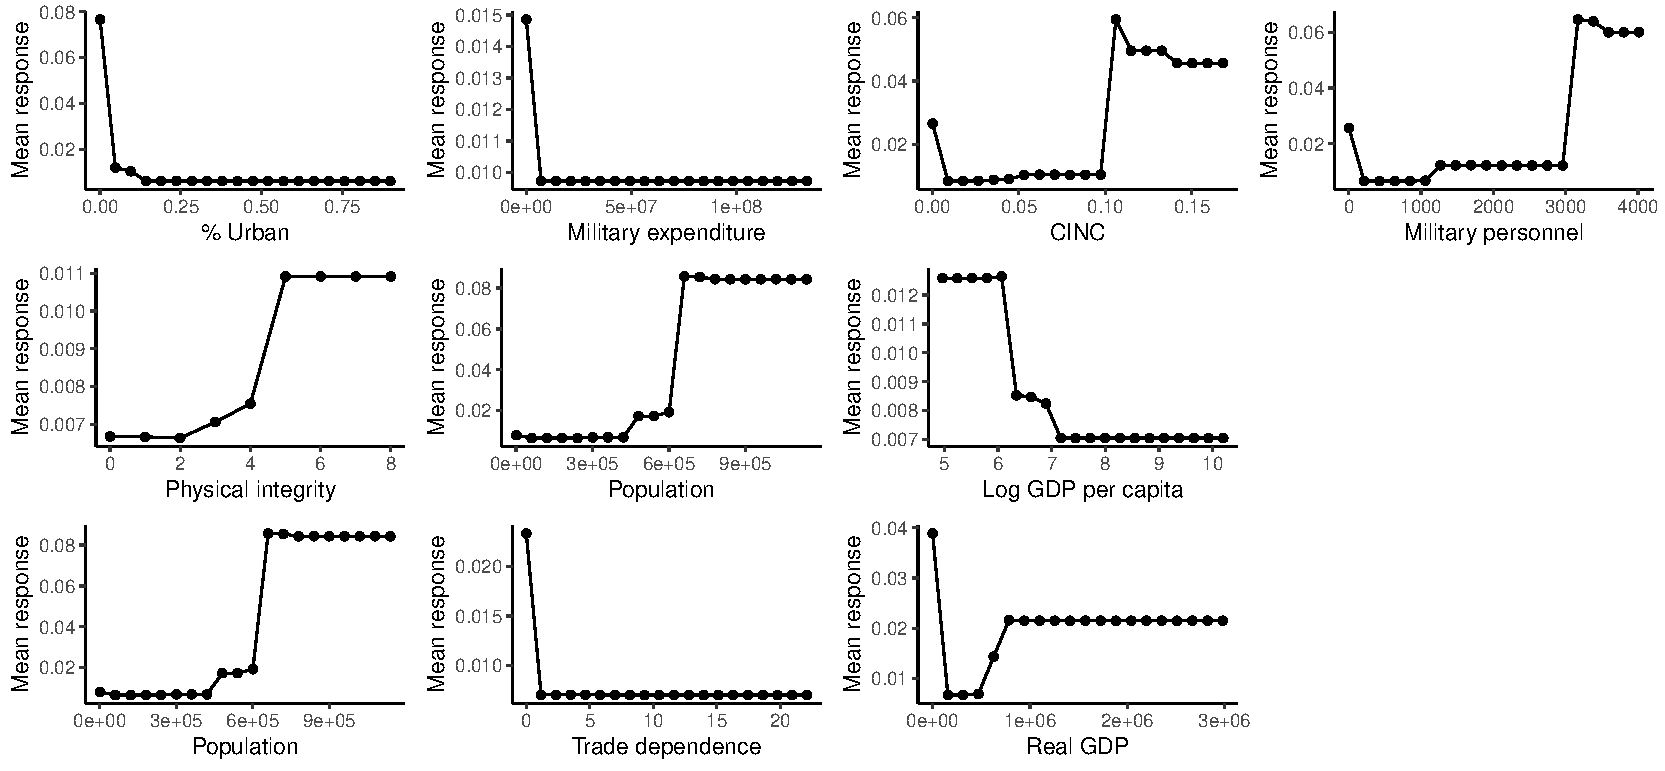
\includegraphics[width=.98\textheight,angle=90]{images/rf-uamk-eth-pd.pdf}
    \caption{Partial Dependence Plot -- Genocides and Politicides during Civil Wars (Cederman et al. Data)}
    \label{fig:rf-mk-ucdp-pd}
\end{figure}

\section{R Code}
\label{sec:mk-code}

The \texttt{R} code below reproduces the analyses presented in this appendix.

\subsection{Data Wrangling}

\scriptsize

\begin{verbatim}
### Load required packages
if (!require("tidyverse")) {
        install.packages("tidyverse")
}
if (!require("data.table")) {
        install.packages("data.table")
}
if (!require("ExtremeBounds")) {
        install.packages("ExtremeBounds")
}
if (!require("sandwich")) {
        install.packages("sandwich")
}
if (!require("h2o")) {
  install.packages("h2o")
}
if (!require("arm")) {
        install.packages("arm")
}

### Load data
setwd("~/Documents/GitHub/mass-killings-8k/") # set the working directory
df <- haven::read_dta("data/base variables.dta") %>% setDT()

### Select and lag variables
sd.cols <- c("UCDPcivilwarstart", "UCDPcivilwarongoing", "COWcivilwarstart",
             "COWcivilwarongoing", "ethnowarstart", "ethnowarongoing",
             "assdummy", "demdummy", "elf", "lmtnest", "pop", "realgdp",
             "rgdppc", "polity2", "exclpop", "discpop", "polrqnew",
             "poltrqnew", "egiptpolrqnew", "egippolrqnew", "discrim",
             "elf2", "interstatewar", "milex", "milper", "percentpopurban",
             "postcoldwar", "coupdummy", "riotdummy", "territoryaims",
             "totaltrade", "tradedependence", "militias", "physint", "cinc",
             "totalbeaths", "guerrilladummy", "change", "sf", "regtrans")

df1 <- cbind(df, df[, shift(.SD, 1, give.names = TRUE),
                    by = ccode, .SDcols = sd.cols]) 

# Remove the second `ccode` variable
df1 <- as.data.frame(df1[, -c(70)])

# Add new variables
df1$logrgdppc_lag_1 <- log(df1$rgdppc_lag_1)
df1$polity2sq_lag_1 <- df1$polity2_lag_1^2

# UCDP civil war == 1
df.ucdp <- df1 %>% filter(UCDPcivilwarongoing == 1)
df.ucdp <- as.data.frame(df.ucdp[, c(1:7, 76:111)])
names(df.ucdp) <- sub("_.*","", names(df.ucdp)) 

# COW civil war == 1
df.cow <- df1 %>% filter(COWcivilwarongoing == 1)
df.cow <- as.data.frame(df.cow[, c(1:7, 76:111)])
names(df.cow) <- sub("_.*","", names(df.cow)) 

# Ethnic civil war == 1
df.eth <- df1 %>% filter(ethnowarongoing == 1)
df.eth <- as.data.frame(df.eth[, c(1:7, 75:110)])
names(df.eth) <- sub("_.*","", names(df.eth)) 

# Regular model
df2 <- as.data.frame(df1[, c(1:7, 70:111)])
names(df2) <- sub("_.*","", names(df2)) 

#### Same procedure with the uamkstart variable

# Preparing the dataset
df3 <- haven::read_dta("data/uamkstart.dta") %>% setDT()
sd.cols <- c("UCDPcivilwarstart", "UCDPcivilwarongoing", "COWcivilwarstart",
             "COWcivilwarongoing", "ethnowarstart", "ethnowarongoing",
             "assdummy", "demdummy", "elf", "lmtnest", "pop", "realgdp",
             "rgdppc", "polity2", "exclpop", "discpop", "polrqnew",
             "poltrqnew", "egiptpolrqnew", "egippolrqnew", "discrim",
             "elf2", "interstatewar", "milex", "milper", "percentpopurban",
             "postcoldwar", "coupdummy", "riotdummy", "territoryaims",
             "totaltrade", "tradedependence", "militias", "physint", "cinc",
             "totalbeaths", "change", "guerrilladummy", "sf", "regtrans")

df4 <- cbind(df3, df3[, shift(.SD, 1, give.names = TRUE),
                    by = ccode, .SDcols = sd.cols]) 

# Remove the second `ccode` variable
df4 <- as.data.frame(df4[, -c(75)])

# Add new variables
df4$logrgdppc_lag_1 <- log(df4$rgdppc_lag_1)
df4$polity2sq_lag_1 <- df4$polity2_lag_1^2

# Renaming variables
df5 <- as.data.frame(df4[, c(1:4, 72:116)])
names(df5) <- sub("_.*","", names(df5)) 

# UCDP civil war == 1
df.ucdp2 <- df5 %>% filter(UCDPcivilwarongoing == 1)
df.ucdp2 <- as.data.frame(df.ucdp2[, c(1:7, 14:49)])
names(df.ucdp2) <- sub("_.*","", names(df.ucdp2)) 

# COW civil war == 1
df.cow2 <- df5 %>% filter(COWcivilwarongoing == 1)
df.cow2 <- as.data.frame(df.cow2[, c(1:7, 14:49)])
names(df.cow2) <- sub("_.*","", names(df.cow2)) 

# Ethnic civil war == 1
df.eth2 <- df5 %>% filter(ethnowarongoing == 1)
df.eth2 <- as.data.frame(df.eth2[, c(1:7, 14:49)])
names(df.eth2) <- sub("_.*","", names(df.eth2)) 
\end{verbatim}

\newpage

\normalsize

\subsection{Extreme Bounds}

\scriptsize

\begin{verbatim}
# Classifying a few variables as mutually exclusive variables.
# "Change" was removed because it was correlated at 0.99 with "regtrans". 
# don't forget to add CINC

free.variables <- c("logrgdppc", "polity2", "mksyr")
civilwar.variables <- c("UCDPcivilwarongoing", "UCDPcivilwarstart",
                        "COWcivilwarongoing", "COWcivilwarstart",
                        "ethnowarongoing", "ethnowarstart")
doubtful.variables <- c("UCDPcivilwarongoing", "UCDPcivilwarstart",
                        "COWcivilwarongoing", "COWcivilwarstart",
                        "ethnowarongoing", "ethnowarstart", "assdummy",
                        "totaltrade", "tradedependence", "milper", "milex",
                        "pop", "totalbeaths", "guerrilladummy", "regtrans",
                        "riotdummy", "territoryaims", "militias",
                        "physint", "percentpopurban", "coupdummy",
                        "postcoldwar",  "lmtnest", "realgdp", "discrim",
                        "exclpop", "discpop", "elf",  "polrqnew",
                        "egippolrqnew", "poltrqnew", "egiptpolrqnew",
                        "polity2sq")

# Cluster-robust standard errors
se.clustered.robust <- function(model.object){
        model.fit <- vcovHC(model.object, type = "HC", cluster = "country")
        out <- sqrt(diag(model.fit))
        return(out)
}

### Models

# Main
m1 <- eba(y = "MKstart", free = free.variables,
          exclusive = list(civilwar.variables),
          doubtful = doubtful.variables, k = 0:4,
          data = df2, vif = 7, level = 0.9,
          se.fun = se.clustered.robust)
save(m1, file = "~/Documents/mk/mk.rda")

# 3 vars at a time
m1 <- eba(y = "MKstart", free = free.variables,
          exclusive = list(civilwar.variables),
          doubtful = doubtful.variables, k = 0:3,
          data = df2, vif = 7, level = 0.9, draws = 10000,
          se.fun = se.clustered.robust)
save(m1, file = "~/Documents/mk/mk-3vars.rda")

# 5 vars at a time
m1 <- eba(y = "MKstart", free = free.variables,
          exclusive = list(civilwar.variables),
          doubtful = doubtful.variables, k = 0:5,
          data = df2, vif = 7, draws = 50000,
          level = 0.9, se.fun = se.clustered.robust)
save(m1, file = "~/Documents/mk/mk-5vars.rda")

# Low VIF
m1 <- eba(y = "MKstart", free = free.variables,
          exclusive = list(civilwar.variables),
          doubtful = doubtful.variables, k = 0:4,
          data = df2, vif = 2.5, level = 0.9,
          draws = 50000,
          se.fun = se.clustered.robust)
save(m1, file = "~/Documents/mk/mk-low-vif.rda")

# High VIF
m1 <- eba(y = "MKstart", free = free.variables,
          exclusive = list(civilwar.variables),
          doubtful = doubtful.variables, k = 0:4,
          data = df2, vif = 10, draws = 50000,
          level = 0.9, se.fun = se.clustered.robust)
save(m1, file = "~/Documents/mk/mk-high-vif.rda")

# No VIF
m1 <- eba(y = "MKstart", free = free.variables,
          exclusive = list(civilwar.variables),
          doubtful = doubtful.variables, k = 0:4,
          data = df2, level = 0.9, draws = 50000,
          se.fun = se.clustered.robust)
save(m1, file = "~/Documents/mk/mk-no-vif.rda")

# Logit
m1 <- eba(y = "MKstart", free = free.variables,
          exclusive = list(civilwar.variables),
          doubtful = doubtful.variables, k = 0:4,
          data = df2, level = 0.9, vif = 7, draws = 50000,
          reg.fun = bayesglm, family = binomial(link = "logit"))
save(m1, file = "~/Documents/mk/mk-logit.rda")

# Probit
m1 <- eba(y = "MKstart", free = free.variables,
          exclusive = list(civilwar.variables),
          doubtful = doubtful.variables, k = 0:4,
          data = df2, level = 0.9, vif = 7, draws = 50000,
          reg.fun = bayesglm, family = binomial(link="probit"))
save(m1, file = "~/Documents/mk/mk-probit.rda")

# CINC
doubtful.variables <- c("UCDPcivilwarongoing", "UCDPcivilwarstart",
                        "COWcivilwarongoing", "COWcivilwarstart",
                        "ethnowarongoing", "ethnowarstart", "assdummy",
                        "totaltrade", "tradedependence", "cinc",
                        "totalbeaths", "guerrilladummy", "regtrans",
                        "riotdummy", "territoryaims", "militias",
                        "physint", "percentpopurban", "coupdummy",
                        "postcoldwar",  "lmtnest", "realgdp", "discrim",
                        "exclpop", "discpop", "elf",  "polrqnew",
                        "egippolrqnew", "poltrqnew", "egiptpolrqnew",
                        "polity2sq")

m1 <- eba(y = "MKstart", free = free.variables,
          exclusive = list(civilwar.variables),
          doubtful = doubtful.variables, k = 0:4,
          data = df2, vif = 7, level = 0.9, 
          se.fun = se.clustered.robust, draws = 50000)
save(m1, file = "~/Documents/mk/mk-cinc.rda")

### Ongoing Civil Wars

# UCDPcivilwarongoing == 1
doubtful.variables <- c("assdummy", "totaltrade", "tradedependence",
                        "milper", "milex", "pop", "totalbeaths",
                        "guerrilladummy", "regtrans", "riotdummy",
                        "territoryaims", "militias", "physint",
                        "percentpopurban", "coupdummy", "postcoldwar",
                        "lmtnest", "realgdp", "discrim", "exclpop",
                        "discpop", "elf",  "polrqnew", "egippolrqnew",
                        "poltrqnew", "egiptpolrqnew", "polity2sq")

m1 <- eba(y = "MKstart", free = free.variables,
          doubtful = doubtful.variables, k = 0:4,
          data = df.ucdp, vif = 7, draws = 50000,
          level = 0.9, se.fun = se.clustered.robust)
save(m1, file = "~/Documents/mk/mk-ucdp.rda")

# COWcivilwarongoing == 1
doubtful.variables <- c("assdummy", "totaltrade", "tradedependence",
                        "milper", "milex", "pop", "totalbeaths",
                        "guerrilladummy", "regtrans", "riotdummy",
                        "territoryaims", "militias", "physint",
                        "percentpopurban", "coupdummy", "postcoldwar",
                        "lmtnest", "realgdp", "discrim", "exclpop",
                        "discpop", "elf",  "polrqnew", "egippolrqnew",
                        "poltrqnew", "egiptpolrqnew", "polity2sq")

m1 <- eba(y = "MKstart", free = free.variables,
          doubtful = doubtful.variables, k = 0:4,
          data = df.cow, vif = 7, draws = 50000,
          level = 0.9, se.fun = se.clustered.robust)
save(m1, file = "~/Documents/mk/mk-cow.rda")

# Ethnic conflict == 1
doubtful.variables <- c("assdummy", "totaltrade", "tradedependence",
                        "milper", "milex", "pop", "totalbeaths",
                        "guerrilladummy", "regtrans", "riotdummy",
                        "territoryaims", "militias", "physint",
                        "percentpopurban", "coupdummy", "postcoldwar",
                        "lmtnest", "realgdp", "discrim", "exclpop", 
                        "discpop", "elf",  "polrqnew", "egippolrqnew",
                        "poltrqnew", "egiptpolrqnew", "polity2sq")

m1 <- eba(y = "MKstart", free = free.variables,
          doubtful = doubtful.variables, k = 0:4,
          data = df.eth, vif = 7, draws = 50000,
          level = 0.9, se.fun = se.clustered.robust)
save(m1, file = "~/Documents/mk/mk-eth.rda")

# Main
free.variables <- c("logrgdppc", "polity2", "uamkyr")
civilwar.variables <- c("UCDPcivilwarongoing", "UCDPcivilwarstart",
                        "COWcivilwarongoing", "COWcivilwarstart",
                        "ethnowarongoing", "ethnowarstart")
doubtful.variables <- c("UCDPcivilwarongoing", "UCDPcivilwarstart",
                        "COWcivilwarongoing", "COWcivilwarstart",
                        "ethnowarongoing", "ethnowarstart", "assdummy",
                        "totaltrade", "tradedependence", "milper", "milex",
                        "pop", "totalbeaths", "guerrilladummy", "regtrans",
                        "riotdummy", "territoryaims", "militias",
                        "physint", "percentpopurban", "coupdummy",
                        "postcoldwar",  "lmtnest", "realgdp", "discrim",
                        "exclpop", "discpop", "elf",  "polrqnew",
                        "egippolrqnew", "poltrqnew", "egiptpolrqnew",
                        "polity2sq")
m1 <- eba(y = "uamkstart", free = free.variables,
          exclusive = list(civilwar.variables),
          doubtful = doubtful.variables, k = 0:4,
          data = df5, vif = 7, level = 0.9, 
          se.fun = se.clustered.robust)
save(m1, file = "~/Documents/mk/uamk.rda")

# 3 vars at a time
m1 <- eba(y = "uamkstart", free = free.variables,
          exclusive = list(civilwar.variables),
          doubtful = doubtful.variables, k = 0:3,
          data = df5, vif = 7, level = 0.9,
          se.fun = se.clustered.robust)
save(m1, file = "~/Documents/mk/uamk-3vars.rda")

# 5 vars at a time
m1 <- eba(y = "uamkstart", free = free.variables,
          exclusive = list(civilwar.variables),
          doubtful = doubtful.variables, k = 0:5,
          data = df5, vif = 7, draws = 50000,
          level = 0.9, se.fun = se.clustered.robust)
save(m1, file = "~/Documents/mk/uamk-5vars.rda")

# Low VIF
m1 <- eba(y = "uamkstart", free = free.variables,
          exclusive = list(civilwar.variables),
          doubtful = doubtful.variables, k = 0:4,
          data = df5, vif = 2.5, level = 0.9, draws = 50000,
          se.fun = se.clustered.robust)
save(m1, file = "~/Documents/mk/uamk-low-vif.rda")

# High VIF
m1 <- eba(y = "uamkstart", free = free.variables,
          exclusive = list(civilwar.variables),
          doubtful = doubtful.variables, k = 0:4,
          data = df5, vif = 10, draws = 50000,
          level = 0.9, se.fun = se.clustered.robust)
save(m1, file = "~/Documents/mk/uamk-high-vif.rda")

# No VIF
m1 <- eba(y = "uamkstart", free = free.variables,
          exclusive = list(civilwar.variables),
          doubtful = doubtful.variables, k = 0:4,
          data = df5, level = 0.9, draws = 50000,
          se.fun = se.clustered.robust)
save(m1, file = "~/Documents/mk/uamk-no-vif.rda")

# Logit
m1 <- eba(y = "uamkstart", free = free.variables,
          exclusive = list(civilwar.variables),
          doubtful = doubtful.variables, k = 0:4,
          data = df5, level = 0.9, vif = 7, draws = 50000,
          reg.fun = bayesglm, family = binomial(link = "logit"))
save(m1, file = "~/Documents/mk/uamk-logit.rda")

# Probit
m1 <- eba(y = "uamkstart", free = free.variables,
          exclusive = list(civilwar.variables),
          doubtful = doubtful.variables, k = 0:4,
          data = df5, level = 0.9, vif = 7, draws = 50000,
          reg.fun = bayesglm, family = binomial(link="probit"))
save(m1, file = "~/Documents/mk/uamk-probit.rda")

# CINC
doubtful.variables <- c("UCDPcivilwarongoing", "UCDPcivilwarstart",
                        "COWcivilwarongoing", "COWcivilwarstart",
                        "ethnowarongoing", "ethnowarstart", "assdummy",
                        "totaltrade", "tradedependence", "cinc",
                        "totalbeaths", "guerrilladummy", "regtrans",
                        "riotdummy", "territoryaims", "militias",
                        "physint", "percentpopurban", "coupdummy",
                        "postcoldwar",  "lmtnest", "realgdp", "discrim",
                        "exclpop", "discpop", "elf",  "polrqnew",
                        "egippolrqnew", "poltrqnew", "egiptpolrqnew",
                        "polity2sq")

m1 <- eba(y = "uamkstart", free = free.variables,
          exclusive = list(civilwar.variables),
          doubtful = doubtful.variables, k = 0:4,
          data = df5, vif = 7, level = 0.9, draws = 50000,
          se.fun = se.clustered.robust)
save(m1, file = "~/Documents/mk/uamk-cinc.rda")

### Ongoing Civil Wars

# UCDPcivilwarongoing == 1
df.ucdp2 <- df5 %>% filter(UCDPcivilwarongoing == 1)
doubtful.variables <- c("assdummy", "totaltrade", "tradedependence",
                        "milper", "milex", "pop", "totalbeaths",
                        "guerrilladummy", "regtrans", "riotdummy",
                        "territoryaims", "militias", "physint",
                        "percentpopurban", "coupdummy", "postcoldwar",
                        "lmtnest", "realgdp", "discrim", "exclpop",
                        "discpop", "elf",  "polrqnew", "egippolrqnew",
                        "poltrqnew", "egiptpolrqnew", "polity2sq")

m1 <- eba(y = "uamkstart", free = free.variables,
          doubtful = doubtful.variables, k = 0:4,
          data = df.ucdp2, vif = 7, draws = 50000,
          level = 0.9, se.fun = se.clustered.robust)
save(m1, file = "~/Documents/mk/uamk-ucdp.rda")

# COWcivilwarongoing == 1
df.cow2 <- df5 %>% filter(COWcivilwarongoing == 1)
doubtful.variables <- c("assdummy", "totaltrade", "tradedependence",
                        "milper", "milex", "pop", "totalbeaths",
                        "guerrilladummy", "regtrans", "riotdummy",
                        "territoryaims", "militias", "physint",
                        "percentpopurban", "coupdummy", "postcoldwar",
                        "lmtnest", "realgdp", "discrim", "exclpop",
                        "discpop", "elf",  "polrqnew", "egippolrqnew",
                        "poltrqnew", "egiptpolrqnew", "polity2sq")

m1 <- eba(y = "uamkstart", free = free.variables,
          doubtful = doubtful.variables, k = 0:4,
          data = df.cow2, vif = 7, draws = 50000,
          level = 0.9, se.fun = se.clustered.robust)
save(m1, file = "~/Documents/mk/uamk-cow.rda")

# Ethnic conflict == 1
df.eth2 <- df5 %>% filter(ethnowarongoing == 1)
doubtful.variables <- c("assdummy", "totaltrade", "tradedependence",
                        "milper", "milex", "pop", "totalbeaths",
                        "guerrilladummy", "regtrans", "riotdummy",
                        "territoryaims", "militias", "physint",
                        "percentpopurban", "coupdummy", "postcoldwar",
                        "lmtnest", "realgdp", "discrim", "exclpop", 
                        "discpop", "elf",  "polrqnew", "egippolrqnew",
                        "poltrqnew", "egiptpolrqnew", "polity2sq")

m1 <- eba(y = "uamkstart", free = free.variables,
          doubtful = doubtful.variables, k = 0:4,
          data = df.eth2, vif = 7, draws = 50000,
          level = 0.9, se.fun = se.clustered.robust)
save(m1, file = "~/Documents/mk/uamk-eth.rda")

### Graphs

# Graphs can be plotted with the code below. 

# Main models
hist(m1, variables = c("logrgdppc", "polity2", "polity2sq", "uamkyr",
                       "UCDPcivilwarongoing",
                       "UCDPcivilwarstart", "COWcivilwarongoing",
                       "COWcivilwarstart", "ethnowarongoing", "ethnowarstart",
                       "assdummy", "totaltrade", "tradedependence", "milper",
                       "milex","pop", "totalbeaths", "guerrilladummy", "regtrans",
                       "riotdummy", "territoryaims", "militias", "physint",
                       "percentpopurban", "coupdummy", "postcoldwar",
                       "lmtnest", "realgdp", "discrim", "exclpop", "discpop",
                       "elf", "polrqnew", "egippolrqnew", "poltrqnew",
                       "egiptpolrqnew"),
     main = c("Log GDP capita", "Polity IV", "Polity IV^2", "Years last genocide",
              "UCDP ongoing", "UCDP onset", "COW ongoing", "COW onset", 
              "Ethnic ongoing", "Ethnic onset", "Assassination", "Total trade", 
              "Trade dependence", "Military personnel", "Military expenditure", "Population", 
              "Total deaths", "Guerrilla", "Regime transition", "Riots",
              "Territory Aims", "Militias", "Physical integrity", "% Urban",
              "Coups", "Post-Cold War", "Mountainous terrain", "Real GDP",
              "Discrimination", "Excl pop", "Discrim pop", "ELF", "Groups/Eth relevant", 
              "Group/Tot pop", "Inc groups/Eth relevant", "Inc groups/Tot pop"),
     density.col = "black", mu.col = "red3")

# Round
m1$coefficients$mean$beta2 <- round(as.numeric(m1$coefficients$mean$beta),4)
m1$coefficients$mean$se2 <- round(as.numeric(m1$coefficients$mean$se),4)
m1$coefficients$mean

## Models including only mass killings during civil wars
hist(m1, variables = c("logrgdppc", "polity2", "polity2sq", "uamkyr",
                       "assdummy", "totaltrade", "tradedependence", "milper",
                       "milex","pop", "totalbeaths", "guerrilladummy", "regtrans",
                       "riotdummy", "territoryaims", "militias", "physint",
                       "percentpopurban", "coupdummy", "postcoldwar",
                       "lmtnest", "realgdp", "discrim", "exclpop", "discpop",
                       "elf", "polrqnew", "egippolrqnew", "poltrqnew",
                       "egiptpolrqnew"),
     main = c("Log GDP capita", "Polity IV", "Polity IV^2", "Years last genocide",
              "Assassination", "Total trade", 
              "Trade dependence", "Military personnel", "Military expenditure", "Population", 
              "Total deaths", "Guerrilla", "Regime transition", "Riots",
              "Territory Aims", "Militias", "Physical integrity", "% Urban",
              "Coups", "Post-Cold War", "Mountainous terrain", "Real GDP",
              "Discrimination", "Excl pop", "Discrim pop", "ELF", "Groups/Eth relevant", 
              "Groups/Tot pop", "Inc groups/Eth relevant", "Inc groups/Tot pop"),
     density.col = "black", mu.col = "red3")
\end{verbatim}

\newpage

\normalsize

\subsection{Random Forests}

\scriptsize

\begin{verbatim}
# Load required package
library(h2o)
h2o.init(nthreads = -1, max_mem_size = "6G") # change min RAM size if necessary

df2a <- as.h2o(df2)

df2a$MKstart <- as.factor(df2a$MKstart)  #encode the binary response as a factor
h2o.levels(df2a$MKstart)

# Partition the data into training, validation and test sets
splits <- h2o.splitFrame(data = df2a, 
                         ratios = 0.75, # train, validation
                         seed = 1234)  # reproducibility


train <- h2o.assign(splits[[1]], "train.hex")   
valid <- h2o.assign(splits[[2]], "valid.hex") 

y <- "MKstart"
x <- setdiff(names(df2), c(y, "ccode", "year", "rgdppc",
                           "mksyr2", "mksyr3", "sf", "country",
                           "elf2", "polity2sq")) 

##########################
### Running the models ###
##########################

rf <- h2o.grid("randomForest", x = x, y = y, training_frame = train, 
               validation_frame = valid, grid_id = "grid01",
               hyper_params = list(ntrees = c(256, 512, 1024),
                                   max_depth = c(10, 20, 40),
                                   mtries = c(5, 6, 7),
                                   balance_classes = c(TRUE, FALSE),
                                   sample_rate = c(0.5, 0.632, 0.95),
                                   col_sample_rate_per_tree = c(0.5, 0.9, 1.0),
                                   histogram_type = "RoundRobin",
                                   seed = 1234)) 

# Saving the most accurate model
rf.grid <- h2o.getGrid(grid_id = "grid01",
                       sort_by = "auc",
                       decreasing = TRUE)

rf2 <- h2o.getModel(rf.grid@model_ids[[1]])
h2o.saveModel(rf2, path = "/Users/politicaltheory/Documents/GitHub/mass-killings-8k/data/")
summary(rf2)
h2o.varimp(rf2)
varimp <- as.data.frame(h2o.varimp(rf2))
h2o.varimp_plot(rf2)

# Second model
rf <- h2o.grid("randomForest", x = x, y = y, training_frame = train, 
               validation_frame = valid, grid_id = "gridrf01b",
               hyper_params = list(ntrees = c(256, 512, 1024),
                                   max_depth = c(10, 20, 40),
                                   mtries = c(5, 6, 7),
                                   balance_classes = c(TRUE, FALSE),
                                   sample_rate = c(0.5, 0.632, 0.95),
                                   col_sample_rate_per_tree = c(0.5, 0.9, 1.0),
                                   histogram_type = "RoundRobin",
                                   seed = 4363))

# Saving the most accurate model
rf.grid <- h2o.getGrid(grid_id = "gridrf01b",
                       sort_by = "auc",
                       decreasing = TRUE)

rf2 <- h2o.getModel(rf.grid@model_ids[[1]])
h2o.saveModel(rf2, path = "/Users/politicaltheory/Documents/GitHub/mass-killings-8k/data/")
summary(rf2)
varimp <- as.data.frame(h2o.varimp(rf2))

# Third model
rf <- h2o.grid("randomForest", x = x, y = y, training_frame = train, 
               validation_frame = valid, grid_id = "gridrf01c",
               hyper_params = list(ntrees = c(256, 512, 1024),
                                   max_depth = c(10, 20, 40),
                                   mtries = c(5, 6, 7),
                                   balance_classes = c(TRUE, FALSE),
                                   sample_rate = c(0.5, 0.632, 0.95),
                                   col_sample_rate_per_tree = c(0.5, 0.9, 1.0),
                                   histogram_type = "RoundRobin",
                                   seed = 7015)) 

# Saving the most accurate model
rf.grid <- h2o.getGrid(grid_id = "gridrf01c",
                       sort_by = "auc",
                       decreasing = TRUE)

rf2 <- h2o.getModel(rf.grid@model_ids[[1]])
h2o.saveModel(rf2, path = "/Users/politicaltheory/Documents/GitHub/mass-killings-8k/data/")
summary(rf2)
varimp <- as.data.frame(h2o.varimp(rf2))
h2o.varimp_plot(rf2)

##########################
### Ongoing civil wars ###
##########################

# UCDP == 1
df.ucdpa <- as.h2o(df.ucdp)

df.ucdpa$MKstart <- as.factor(df.ucdpa$MKstart)  #encode the binary repsonse as a factor
h2o.levels(df.ucdpa$MKstart)

# Partition the data into training, validation and test sets
splits <- h2o.splitFrame(data = df.ucdpa, 
                         ratios = 0.75, 
                         seed = 1234)  


train <- h2o.assign(splits[[1]], "train.hex")   
valid <- h2o.assign(splits[[2]], "valid.hex") 

y <- "MKstart"
x <- setdiff(names(df.ucdp), c(y, "ccode", "year", "rgdppc",
                           "mksyr2", "mksyr3", "sf", "country",
                           "elf2", "polity2sq")) 

# Running the model
rf <- h2o.grid("randomForest", x = x, y = y, training_frame = train, 
               validation_frame = valid,  grid_id = "grid02",
               hyper_params = list(ntrees = c(256, 512, 1024),
                                   max_depth = c(10, 20, 40),
                                   mtries = c(5, 6, 7),
                                   balance_classes = c(TRUE, FALSE),
                                   sample_rate = c(0.5, 0.632, 0.95),
                                   col_sample_rate_per_tree = c(0.5, 0.9, 1.0),
                                   histogram_type = "RoundRobin",
                                   seed = 1234)) 

rf.grid <- h2o.getGrid(grid_id = "grid02",
                       sort_by = "auc",
                       decreasing = TRUE)
rf2 <- h2o.getModel(rf.grid@model_ids[[1]])
h2o.saveModel(rf2, path = "/Users/politicaltheory/Documents/GitHub/mass-killings-8k/data/")
summary(rf2)
h2o.varimp_plot(rf2)

# COW == 1
df.cowa <- as.h2o(df.cow)

df.cowa$MKstart <- as.factor(df.cowa$MKstart)  #encode the binary repsonse as a factor
h2o.levels(df.cowa$MKstart)

# Partition the data into training, validation and test sets
splits <- h2o.splitFrame(data = df.cowa, 
                         ratios = 0.75,  
                         seed = 1234)  


train <- h2o.assign(splits[[1]], "train.hex")   
valid <- h2o.assign(splits[[2]], "valid.hex") 

y <- "MKstart"
x <- setdiff(names(df.ucdp), c(y, "ccode", "year", "rgdppc",
                               "mksyr2", "mksyr3", "sf", "country",
                               "elf2", "polity2sq")) 

# Running the model
rf <- h2o.grid("randomForest", x = x, y = y, training_frame = train, 
               validation_frame = valid, grid_id = "gridrf03",
               hyper_params = list(ntrees = c(256, 512, 1024),
                                   max_depth = c(10, 20, 40),
                                   mtries = c(5, 6, 7),
                                   balance_classes = c(TRUE, FALSE),
                                   sample_rate = c(0.5, 0.632, 0.95),
                                   col_sample_rate_per_tree = c(0.5, 0.9, 1.0),
                                   histogram_type = "RoundRobin",
                                   seed = 1234)) 

rf.grid <- h2o.getGrid(grid_id = "gridrf03",
                       sort_by = "auc",
                       decreasing = TRUE)
rf2 <- h2o.getModel(rf.grid@model_ids[[1]])
h2o.saveModel(rf2, path = "/Users/politicaltheory/Documents/GitHub/mass-killings-8k/data/")
summary(rf2)
varimp <- as.data.frame(h2o.varimp(rf2))
h2o.varimp_plot(rf2)

# Ethnic conflict == 1
df.etha <- as.h2o(df.eth)

df.etha$MKstart <- as.factor(df.etha$MKstart)  #encode the binary repsonse as a factor
h2o.levels(df.etha$MKstart)

# Partition the data into training, validation and test sets
splits <- h2o.splitFrame(data = df.etha, 
                         ratios = 0.75,  
                         seed = 1234)  


train <- h2o.assign(splits[[1]], "train.hex")   
valid <- h2o.assign(splits[[2]], "valid.hex") 

y <- "MKstart"
x <- setdiff(names(df.eth), c(y, "ccode", "year", "rgdppc",
                               "mksyr2", "mksyr3", "sf", "country",
                               "elf2", "polity2sq")) 

# Running the model
rf <- h2o.grid("randomForest", x = x, y = y, training_frame = train, 
               validation_frame = valid, grid_id = "gridrf04",
               hyper_params = list(ntrees = c(256, 512, 1024),
                                   max_depth = c(10, 20, 40),
                                   mtries = c(5, 6, 7),
                                   balance_classes = c(TRUE, FALSE),
                                   sample_rate = c(0.5, 0.632, 0.95),
                                   col_sample_rate_per_tree = c(0.5, 0.9, 1.0),
                                   histogram_type = "RoundRobin",
                                   seed = 1234)) 

rf.grid <- h2o.getGrid(grid_id = "gridrf04",
                       sort_by = "auc",
                       decreasing = TRUE)
rf2 <- h2o.getModel(rf.grid@model_ids[[1]])
h2o.saveModel(rf2, path = "/Users/politicaltheory/Documents/GitHub/mass-killings-8k/data/")
summary(rf2)
varimp <- as.data.frame(h2o.varimp(rf2))
h2o.varimp_plot(rf2)

###########################################################
## Same models with Genocide/Politicide variable (Harf) ###
###########################################################
df5a <- as.h2o(df5)

df5a$uamkstart <- as.factor(df5a$uamkstart)  #encode the binary repsonse as a factor
h2o.levels(df5a$uamkstart)

# Partition the data into training, validation and test sets
splits <- h2o.splitFrame(data = df5a, 
                         ratios = 0.75, 
                         seed = 1234) 


train <- h2o.assign(splits[[1]], "train.hex")   
valid <- h2o.assign(splits[[2]], "valid.hex") 

y <- "uamkstart"
x <- setdiff(names(df5), c(y, "ccode", "year", "rgdppc",
                           "uamkyr2", "uamkyr3", "sf", "country",
                           "elf2", "polity2sq")) 

# Main model
rf <- h2o.grid("randomForest", x = x, y = y, training_frame = train, 
               validation_frame = valid, grid_id = "gridrf05",
               hyper_params = list(ntrees = c(256, 512, 1024),
                                   max_depth = c(10, 20, 40),
                                   mtries = c(5, 6, 7),
                                   balance_classes = c(TRUE, FALSE),
                                   sample_rate = c(0.5, 0.632, 0.95),
                                   col_sample_rate_per_tree = c(0.5, 0.9, 1.0),
                                   histogram_type = "RoundRobin",
                                   seed = 1234)) 

# Saving the most accurate model
rf.grid <- h2o.getGrid(grid_id = "gridrf05",
                       sort_by = "auc",
                       decreasing = TRUE)

rf2 <- h2o.getModel(rf.grid@model_ids[[1]])
h2o.saveModel(rf2, path = "/Users/politicaltheory/Documents/GitHub/mass-killings-8k/data/")
summary(rf2)
varimp <- as.data.frame(h2o.varimp(rf2))
h2o.varimp_plot(rf2)

# UCDP == 1
df.ucdp2a <- as.h2o(df.ucdp2)

df.ucdp2a$uamkstart <- as.factor(df.ucdp2a$uamkstart)  #encode the binary repsonse as a factor
h2o.levels(df.ucdp2a$uamkstart)

# Partition the data into training, validation and test sets
splits <- h2o.splitFrame(data = df.ucdp2a, 
                         ratios = 0.75, 
                         seed = 1234) 


train <- h2o.assign(splits[[1]], "train.hex")   
valid <- h2o.assign(splits[[2]], "valid.hex") 

y <- "uamkstart"
x <- setdiff(names(df.ucdp2), c(y, "ccode", "year", "rgdppc",
                           "uamkyr2", "uamkyr3", "sf", "country",
                           "elf2", "polity2sq")) 

# Running the model
rf <- h2o.grid("randomForest", x = x, y = y, training_frame = train, 
               validation_frame = valid, grid_id = "gridrf06",
               hyper_params = list(ntrees = c(256, 512, 1024),
                                   max_depth = c(10, 20, 40),
                                   mtries = c(5, 6, 7),
                                   balance_classes = c(TRUE, FALSE),
                                   sample_rate = c(0.5, 0.632, 0.95),
                                   col_sample_rate_per_tree = c(0.5, 0.9, 1.0),
                                   histogram_type = "RoundRobin",
                                   seed = 1234)) 

rf.grid <- h2o.getGrid(grid_id = "gridrf06",
                       sort_by = "auc",
                       decreasing = TRUE)
rf2 <- h2o.getModel(rf.grid@model_ids[[1]])
h2o.saveModel(rf2, path = "/Users/politicaltheory/Documents/GitHub/mass-killings-8k/data/")
summary(rf2)
varimp <- as.data.frame(h2o.varimp(rf2))
h2o.varimp_plot(rf2)

# COW == 1
df.cow2a <- as.h2o(df.cow2)

df.cow2a$uamkstart <- as.factor(df.cow2a$uamkstart)  #encode the binary repsonse as a factor
h2o.levels(df.cow2a$uamkstart)

# Partition the data into training, validation and test sets
splits <- h2o.splitFrame(data = df.cow2a, 
                         ratios = 0.75,  
                         seed = 1234)  


train <- h2o.assign(splits[[1]], "train.hex")   
valid <- h2o.assign(splits[[2]], "valid.hex") 

y <- "uamkstart"
x <- setdiff(names(df.cow2), c(y, "ccode", "year", "rgdppc",
                           "uamkyr2", "uamkyr3", "sf", "country",
                           "elf2", "polity2sq")) 

# Running the model
rf <- h2o.grid("randomForest", x = x, y = y, training_frame = train, 
               validation_frame = valid, grid_id = "gridrf07",
               hyper_params = list(ntrees = c(256, 512, 1024),
                                   max_depth = c(10, 20, 40),
                                   mtries = c(5, 6, 7),
                                   balance_classes = c(TRUE, FALSE),
                                   sample_rate = c(0.5, 0.632, 0.95),
                                   col_sample_rate_per_tree = c(0.5, 0.9, 1.0),
                                   histogram_type = "RoundRobin",
                                   seed = 1234)) 

rf.grid <- h2o.getGrid(grid_id = "gridrf07",
                       sort_by = "auc",
                       decreasing = TRUE)
rf2 <- h2o.getModel(rf.grid@model_ids[[1]])
h2o.saveModel(rf2, path = "/Users/politicaltheory/Documents/GitHub/mass-killings-8k/data/")
summary(rf2)
varimp <- as.data.frame(h2o.varimp(rf2))
h2o.varimp_plot(rf2)

# Ethnic conflict == 1
df.eth2a <- as.h2o(df.eth2)

df.eth2a$uamkstart <- as.factor(df.eth2a$uamkstart)  #encode the binary repsonse as a factor
h2o.levels(df.eth2a$uamkstart)

# Partition the data into training, validation and test sets
splits <- h2o.splitFrame(data = df.eth2a, 
                         ratios = 0.75, 
                         seed = 1234) 


train <- h2o.assign(splits[[1]], "train.hex")   
valid <- h2o.assign(splits[[2]], "valid.hex") 

y <- "uamkstart"
x <- setdiff(names(df.eth2), c(y, "ccode", "year", "rgdppc",
                           "uamkyr2", "uamkyr3", "sf", "country",
                           "elf2", "polity2sq")) 

# Running the model
rf <- h2o.grid("randomForest", x = x, y = y, training_frame = train, 
               validation_frame = valid, grid_id = "gridrf08",
               hyper_params = list(ntrees = c(256, 512, 1024),
                                   max_depth = c(10, 20, 40),
                                   mtries = c(5, 6, 7),
                                   balance_classes = c(TRUE, FALSE),
                                   sample_rate = c(0.5, 0.632, 0.95),
                                   col_sample_rate_per_tree = c(0.5, 0.9, 1.0),
                                   histogram_type = "RoundRobin",
                                   seed = 1234)) 

rf.grid <- h2o.getGrid(grid_id = "gridrf08",
                       sort_by = "auc",
                       decreasing = TRUE)
rf2 <- h2o.getModel(rf.grid@model_ids[[1]])
h2o.saveModel(rf2, path = "/Users/politicaltheory/Documents/GitHub/mass-killings-8k/data/")
summary(rf2)
varimp <- as.data.frame(h2o.varimp(rf2))
h2o.varimp_plot(rf2)


###############
### Graphs ####
###############

# Main model
library(h2o)
h2o.init(nthreads = -1, max_mem_size = "6G") 
a <- h2o.loadModel("grid01_model_197")
print(va <- a %>% h2o.varimp() %>% as.data.frame() %>% head(., 10))

df2a <- as.h2o(df2)

df2a$MKstart <- as.factor(df2a$MKstart)  #encode the binary repsonse as a factor
h2o.levels(df2a$MKstart)

# Partition the data into training, validation and test sets
splits <- h2o.splitFrame(data = df2a, 
                         ratios = 0.75,  # 70%, 15%, 15%
                         seed = 1234)  # reproducibility


train <- h2o.assign(splits[[1]], "train.hex")   
valid <- h2o.assign(splits[[2]], "valid.hex") 

y <- "MKstart"
x <- setdiff(names(df2), c(y, "ccode", "year", "rgdppc",
                           "mksyr2", "mksyr3", "sf", "country",
                           "elf2", "polity2sq"))  

# Variable Importance
par(mgp=c(2.2,0.45,0), tcl=-0.4, mar=c(2,7.5,1,1))
barplot(va$scaled_importance[10:1],
        horiz = TRUE, las = 1, cex.names=0.9,
        names.arg = c("Real GDP",
                      "Total trade",
                      "Polity IV",
                      "Population", 
                      "Military expenditure",
                      "Military personnel",
                      "Trade dependence", 
                      "% Urban pop.",
                      "Log GDP per capita",
                      "Years mass killing"),
        main = "")


# Partial dependence plots
mksyr <- h2o.partialPlot(object = a, data = train, cols = c("mksyr"), plot_stddev = F)
p1 <- qplot(mksyr$mksyr, mksyr$mean_response) + geom_line() + theme_classic() +
        xlab("Years mass killing") +  ylab("Mean response")

logrgdppc <- h2o.partialPlot(object = a, data = train, cols = c("logrgdppc"), plot_stddev = F)
p2 <- qplot(logrgdppc$logrgdppc, logrgdppc$mean_response) + geom_line() + theme_classic() +
  xlab("Log GDP per capita") +  ylab("Mean response")

percentpopurban <- h2o.partialPlot(object = a, data = train, cols = c("percentpopurban"), plot_stddev = F)
p3 <- qplot(percentpopurban$percentpopurban, percentpopurban$mean_response) + geom_line() +
        theme_classic() + xlab("% Urban pop.") + ylab("Mean response")

tradedependence <- h2o.partialPlot(object = a, data = train, cols = c("tradedependence"), plot_stddev = F)
p4 <- qplot(tradedependence$tradedependence, tradedependence$mean_response) + geom_line() +
        theme_classic() + xlab("Trade dependence") + ylab("Mean response")

milper <- h2o.partialPlot(object = a, data = train, cols = c("milper"), plot_stddev = F)
p5 <- qplot(milper$milper, milper$mean_response) + geom_line() + theme_classic() +
        xlab("Military personnel") + ylab("Mean response")

milex <- h2o.partialPlot(object = a, data = train, cols = c("milex"), plot_stddev = F)
p6 <- qplot(milex$milex, milex$mean_response) + geom_line() + theme_classic() +
  xlab("Military expenditure") + ylab("Mean response")

pop <- h2o.partialPlot(object = a, data = train, cols = c("pop"), plot_stddev = F)
p7 <- qplot(pop$pop, pop$mean_response) + geom_line() + theme_classic() +
        xlab("Population") + ylab("Mean response")

polity2 <- h2o.partialPlot(object = a, data = train, cols = c("polity2"), plot_stddev = F)
p8 <- qplot(polity2$polity2, polity2$mean_response) + geom_line() + theme_classic() +
  xlab("Polity IV") + ylab("Mean response")

totaltrade <- h2o.partialPlot(object = a, data = train, cols = c("totaltrade"), plot_stddev = F)
p9 <- qplot(totaltrade$totaltrade, totaltrade$mean_response) + geom_line() + theme_classic() +
  xlab("Total trade") + ylab("Mean response")

realgdp <- h2o.partialPlot(object = a, data = train, cols = c("realgdp"), plot_stddev = F)
p10 <- qplot(realgdp$realgdp, realgdp$mean_response) + geom_line() + theme_classic() +
  xlab("Real GDP") + ylab("Mean response")

# Multiplot function: http://www.cookbook-r.com/Graphs/Multiple_graphs_on_one_page_(ggplot2)/
multiplot <- function(..., plotlist=NULL, file, cols=1, layout=NULL) {
        library(grid)
        
        # Make a list from the ... arguments and plotlist
        plots <- c(list(...), plotlist)
        
        numPlots = length(plots)
        
        # If layout is NULL, then use 'cols' to determine layout
        if (is.null(layout)) {
                # Make the panel
                # ncol: Number of columns of plots
                # nrow: Number of rows needed, calculated from # of cols
                layout <- matrix(seq(1, cols * ceiling(numPlots/cols)),
                                 ncol = cols, nrow = ceiling(numPlots/cols))
        }
        
        if (numPlots==1) {
                print(plots[[1]])
                
        } else {
                # Set up the page
                grid.newpage()
                pushViewport(viewport(layout = grid.layout(nrow(layout), ncol(layout))))
                
                # Make each plot, in the correct location
                for (i in 1:numPlots) {
                        # Get the i,j matrix positions of the regions that contain this subplot
                        matchidx <- as.data.frame(which(layout == i, arr.ind = TRUE))
                        
                        print(plots[[i]], vp = viewport(layout.pos.row = matchidx$row,
                                                        layout.pos.col = matchidx$col))
                }
        }
}

multiplot(p1,p5,p8,p2,p6,p9,p3,p7,p10,p4, cols = 4)  # 11.1x5.14 in

#######################################
### Mass killings during civil wars ###
#######################################

# UCDP == 1
a <- h2o.loadModel("grid02_model_349")
print(va <- a %>% h2o.varimp() %>% as.data.frame() %>% head(., 10)) 

par(mgp=c(2.2,0.45,0), tcl=-0.4, mar=c(2,7.5,1,1))
barplot(va$scaled_importance[10:1],
        horiz = TRUE, las = 1, cex.names=0.9,
        names.arg = c("Real GDP",
                      "Military personnel",
                      "Population",
                      "Military expenditure",
                      "Total trade",
                      "Log GDP per capita",
                      "CINC",
                      "Years mass killing",
                      "Trade dependence",
                      "% Urban pop."),
        main = "")

df.ucdpa <- as.h2o(df.ucdp)

df.ucdpa$MKstart <- as.factor(df.ucdpa$MKstart)  #encode the binary repsonse as a factor
h2o.levels(df.ucdpa$MKstart)

# Partition the data into training, validation and test sets
splits <- h2o.splitFrame(data = df.ucdpa, 
                         ratios = 0.75,  # 70%, 15%, 15%
                         seed = 1234)  # reproducibility


train <- h2o.assign(splits[[1]], "train.hex")   
valid <- h2o.assign(splits[[2]], "valid.hex") 

y <- "MKstart"
x <- setdiff(names(df.ucdp), c(y, "ccode", "year", "rgdppc",
                               "mksyr2", "mksyr3", "sf", "country",
                               "elf2", "polity2sq")) 

percentpopurban <- h2o.partialPlot(object = a, data = train, cols = c("percentpopurban"), plot_stddev = F)
p1 <- qplot(percentpopurban$percentpopurban, percentpopurban$mean_response) + geom_line() +
        theme_classic() + xlab("% Urban") + ylab("Mean response")

tradedependence <- h2o.partialPlot(object = a, data = train, cols = c("tradedependence"), plot_stddev = F)
p2 <- qplot(tradedependence$tradedependence, tradedependence$mean_response) + geom_line() +
  theme_classic() + xlab("Trade dependence") + ylab("Mean response")

mksyr <- h2o.partialPlot(object = a, data = train, cols = c("mksyr"), plot_stddev = F)
p3 <- qplot(mksyr$mksyr, mksyr$mean_response) + geom_line() + theme_classic() + 
  xlab("Years since mass killing") +  ylab("Mean response")

cinc <- h2o.partialPlot(object = a, data = train, cols = c("cinc"), plot_stddev = F)
p4 <- qplot(cinc$cinc, cinc$mean_response) + geom_line() + theme_classic() + 
  xlab("CINC") +  ylab("Mean response")

logrgdppc <- h2o.partialPlot(object = a, data = train, cols = c("logrgdppc"), plot_stddev = F)
p5 <- qplot(logrgdppc$logrgdppc, logrgdppc$mean_response) + geom_line() + theme_classic() +
        xlab("Log GDP per capita") + ylab("Mean response")

totaltrade <- h2o.partialPlot(object = a, data = train, cols = c("totaltrade"), plot_stddev = F)
p6 <- qplot(totaltrade$totaltrade, totaltrade$mean_response) + geom_line() + theme_classic() +
        xlab("Total trade") + ylab("Mean response")

milex <- h2o.partialPlot(object = a, data = train, cols = c("milex"), plot_stddev = F)
p7 <- qplot(milex$milex, milex$mean_response) + geom_line() + theme_classic() +
  xlab("Military expenditure") + ylab("Mean response")

pop <- h2o.partialPlot(object = a, data = train, cols = c("pop"), plot_stddev = F)
p8 <- qplot(pop$pop, pop$mean_response) + geom_line() + theme_classic() +
  xlab("Population") + ylab("Mean response")

milper <- h2o.partialPlot(object = a, data = train, cols = c("milper"), plot_stddev = F)
p9 <- qplot(milper$milper, milper$mean_response) + geom_line() + theme_classic() +
  xlab("Military personnel") + ylab("Mean response")

realgdp <- h2o.partialPlot(object = a, data = train, cols = c("realgdp"), plot_stddev = F)
p10 <- qplot(realgdp$realgdp, realgdp$mean_response) + geom_line() + theme_classic() +
  xlab("Real GDP") + ylab("Mean response")

multiplot(p1,p5,p8,p2,p6,p9,p3,p7,p10,p4, cols = 4)  # 11.09x5.14 in


# COW == 1
a <- h2o.loadModel("gridrf03_model_41")
print(va <- a %>% h2o.varimp() %>% as.data.frame() %>% head(., 10)) 

par(mgp=c(2.2,0.45,0), tcl=-0.4, mar=c(2,7.5,1,1))
barplot(va$scaled_importance[10:1],
        horiz = TRUE, las = 1, cex.names=0.9,
        names.arg = c("Polarisation",
                      "Military expenditure",
                      "Military personnel",
                      "Excluded population", 
                      "% Urban",
                      "Previous riots",
                      "Total battle deaths", 
                      "Log GDP per capita",
                      "Years mass killing",
                      "Physical integrity"),
        main = "")

df.cowa <- as.h2o(df.cow)

df.cowa$MKstart <- as.factor(df.cowa$MKstart)  #encode the binary repsonse as a factor
h2o.levels(df.cowa$MKstart)

# Partition the data into training, validation and test sets
splits <- h2o.splitFrame(data = df.cowa, 
                         ratios = 0.75,  
                         seed = 1234) 


train <- h2o.assign(splits[[1]], "train.hex")   
valid <- h2o.assign(splits[[2]], "valid.hex") 

y <- "MKstart"
x <- setdiff(names(df.ucdp), c(y, "ccode", "year", "rgdppc",
                               "mksyr2", "mksyr3", "sf", "country",
                               "elf2", "polity2sq")) 

physint <- h2o.partialPlot(object = a, data = train, cols = c("physint"), plot_stddev = F)
p1 <- qplot(physint$physint, physint$mean_response) + geom_line() + theme_classic() + 
        xlab("Physical integrity") +  ylab("Mean response")

mksyr <- h2o.partialPlot(object = a, data = train, cols = c("mksyr"), plot_stddev = F)
p2 <- qplot(mksyr$mksyr, mksyr$mean_response) + geom_line() + theme_classic() + 
  xlab("Years mass killing") +  ylab("Mean response")

logrgdppc <- h2o.partialPlot(object = a, data = train, cols = c("logrgdppc"), plot_stddev = F)
p3 <- qplot(logrgdppc$logrgdppc, logrgdppc$mean_response) + geom_line() + theme_classic() +
        xlab("Log GDP per capita") + ylab("Mean response")

totalbeaths <- h2o.partialPlot(object = a, data = train, cols = c("totalbeaths"), plot_stddev = F)
p4 <- qplot(totalbeaths$totalbeaths, totalbeaths$mean_response) + geom_line() + theme_classic() +
  xlab("Total battle deaths") + ylab("Mean response")

riotdummy <- h2o.partialPlot(object = a, data = train, cols = c("riotdummy"), plot_stddev = F)
p5 <- qplot(riotdummy$riotdummy, riotdummy$mean_response) + geom_line() + theme_classic() +
        xlab("Previous riots") + ylab("Mean response")

percentpopurban <- h2o.partialPlot(object = a, data = train, cols = c("percentpopurban"), plot_stddev = F)
p6 <- qplot(percentpopurban$percentpopurban, percentpopurban$mean_response) + geom_line() +
  theme_classic() + xlab("% Urban") + ylab("Mean response")

exclpop <- h2o.partialPlot(object = a, data = train, cols = c("exclpop"), plot_stddev = F)
p7 <- qplot(exclpop$exclpop, exclpop$mean_response) + geom_line() +
  theme_classic() + xlab("Excluded population") + ylab("Mean response")

milper <- h2o.partialPlot(object = a, data = train, cols = c("milper"), plot_stddev = F)
p8 <- qplot(milper$milper, milper$mean_response) + geom_line() + theme_classic() +
  xlab("Military personnel") + ylab("Mean response")

milex <- h2o.partialPlot(object = a, data = train, cols = c("milex"), plot_stddev = F)
p9 <- qplot(milex$milex, milex$mean_response) + geom_line() + theme_classic() +
  xlab("Military expenditure") + ylab("Mean response")

egiptpolrqnew <- h2o.partialPlot(object = a, data = train, cols = c("egiptpolrqnew"), plot_stddev = F)
p10 <- qplot(egiptpolrqnew$egiptpolrqnew, egiptpolrqnew$mean_response) + geom_line() + theme_classic() +
  xlab("Polarisation") + ylab("Mean response")

multiplot(p1,p5,p8,p2,p6,p9,p3,p7,p10,p4, cols = 4)  # 11.09x5.14 in

# Ethnic conflict == 1
a <- h2o.loadModel("gridrf04_model_52")
print(va <- a %>% h2o.varimp() %>% as.data.frame() %>% head(., 10)) 

par(mgp=c(2.2,0.45,0), tcl=-0.4, mar=c(2,7.5,1,1))
barplot(va$scaled_importance[10:1],
        horiz = TRUE, las = 1, cex.names=0.9,
        names.arg = c("Log GDP per capita",
                      "Democracy",
                      "Years mass killing",
                      "Polarisation",
                      "% Urban",
                      "Territorial aims", 
                      "Trade dependence",
                      "Excluded population",
                      "Military personnel",
                      "Polity IV"),
        main = "")

df.etha <- as.h2o(df.eth)

df.etha$MKstart <- as.factor(df.etha$MKstart)  #encode the binary repsonse as a factor
h2o.levels(df.etha$MKstart)

# Partition the data into training, validation and test sets
splits <- h2o.splitFrame(data = df.etha, 
                         ratios = 0.75, 
                         seed = 42)  


train <- h2o.assign(splits[[1]], "train.hex")   
valid <- h2o.assign(splits[[2]], "valid.hex") 

y <- "MKstart"
x <- setdiff(names(df.ucdp), c(y, "ccode", "year", "rgdppc",
                               "mksyr2", "mksyr3", "sf", "country",
                               "elf2", "polity2sq")) 

polity2 <- h2o.partialPlot(object = a, data = train, cols = c("polity2"), plot_stddev = F)
p1 <- qplot(polity2$polity2, polity2$mean_response) + geom_line() + theme_classic() + 
        xlab("Polity IV") +  ylab("Mean response")

milper <- h2o.partialPlot(object = a, data = train, cols = c("milper"), plot_stddev = F)
p2 <- qplot(milper$milper, milper$mean_response) + geom_line() + theme_classic() +
  xlab("Military personnel") + ylab("Mean response")

exclpop <- h2o.partialPlot(object = a, data = train, cols = c("exclpop"), plot_stddev = F)
p3 <- qplot(exclpop$exclpop, exclpop$mean_response) + geom_line() +
  theme_classic() + xlab("Excluded population") + ylab("Mean response")

tradedependence <- h2o.partialPlot(object = a, data = train, cols = c("tradedependence"), plot_stddev = F)
p4 <- qplot(tradedependence$tradedependence, tradedependence$mean_response) + geom_line() +
  theme_classic() + xlab("Trade dependence") + ylab("Mean response")

territoryaims <- h2o.partialPlot(object = a, data = train, cols = c("territoryaims"), plot_stddev = F)
p5 <- qplot(territoryaims$territoryaims, territoryaims$mean_response) + geom_line() +
  theme_classic() + xlab("Territory aims") + ylab("Mean response")

percentpopurban <- h2o.partialPlot(object = a, data = train, cols = c("percentpopurban"), plot_stddev = F)
p6 <- qplot(percentpopurban$percentpopurban, percentpopurban$mean_response) + geom_line() +
  theme_classic() + xlab("% Urban") + ylab("Mean response")

egiptpolrqnew <- h2o.partialPlot(object = a, data = train, cols = c("egiptpolrqnew"), plot_stddev = F)
p7 <- qplot(egiptpolrqnew$egiptpolrqnew, egiptpolrqnew$mean_response) + geom_line() + theme_classic() +
  xlab("Polarisation") + ylab("Mean response")

mksyr <- h2o.partialPlot(object = a, data = train, cols = c("mksyr"), plot_stddev = F)
p8 <- qplot(mksyr$mksyr, mksyr$mean_response) + geom_line() + theme_classic() + 
  xlab("Years mass killing") +  ylab("Mean response")

demdummy <- h2o.partialPlot(object = a, data = train, cols = c("demdummy"), plot_stddev = F)
p9 <- qplot(demdummy$demdummy, demdummy$mean_response) + geom_line() + theme_classic() + 
  xlab("Democracy") +  ylab("Mean response")

logrgdppc <- h2o.partialPlot(object = a, data = train, cols = c("logrgdppc"), plot_stddev = F)
p10 <- qplot(logrgdppc$logrgdppc, logrgdppc$mean_response) + geom_line() + theme_classic() +
  xlab("Log GDP per capita") + ylab("Mean response")

multiplot(p1,p5,p8,p2,p6,p9,p3,p7,p10,p4, cols = 4)  # 11.09x5.14 in

#######################
### Different seeds ###
#######################

## Seed 4363
a <- h2o.loadModel("gridrf01b_model_73")
print(va <- a %>% h2o.varimp() %>% as.data.frame() %>% head(., 10))

df2a <- as.h2o(df2)

df2a$MKstart <- as.factor(df2a$MKstart)  #encode the binary repsonse as a factor
h2o.levels(df2a$MKstart)

# Partition the data into training, validation and test sets
splits <- h2o.splitFrame(data = df2a, 
                         ratios = 0.75,  # 70%, 15%, 15%
                         seed = 1234)  # reproducibility


train <- h2o.assign(splits[[1]], "train.hex")   
valid <- h2o.assign(splits[[2]], "valid.hex") 

y <- "MKstart"
x <- setdiff(names(df2), c(y, "ccode", "year", "rgdppc",
                           "mksyr2", "mksyr3", "sf", "country",
                           "elf2", "polity2sq"))  

# Variable Importance
par(mgp=c(2.2,0.45,0), tcl=-0.4, mar=c(2,7.5,1,1))
barplot(va$scaled_importance[10:1],
        horiz = TRUE, las = 1, cex.names=0.9,
        names.arg = c("Total trade",
                      "Real GDP",
                      "CINC",
                      "Population", 
                      "Military personnel",
                      "Military expenditure",
                      "Years mass killing",
                      "% Urban pop.",
                      "Trade dependence", 
                      "Log GDP per capita"),
        main = "")


# Partial dependence plots
logrgdppc <- h2o.partialPlot(object = a, data = train, cols = c("logrgdppc"), plot_stddev = F)
p1 <- qplot(logrgdppc$logrgdppc, logrgdppc$mean_response) + geom_line() + theme_classic() +
  xlab("Log GDP per capita") +  ylab("Mean response")

tradedependence <- h2o.partialPlot(object = a, data = train, cols = c("tradedependence"), plot_stddev = F)
p2 <- qplot(tradedependence$tradedependence, tradedependence$mean_response) + geom_line() +
  theme_classic() + xlab("Trade dependence") + ylab("Mean response")

percentpopurban <- h2o.partialPlot(object = a, data = train, cols = c("percentpopurban"), plot_stddev = F)
p3 <- qplot(percentpopurban$percentpopurban, percentpopurban$mean_response) + geom_line() +
  theme_classic() + xlab("% Urban pop.") + ylab("Mean response")

mksyr <- h2o.partialPlot(object = a, data = train, cols = c("mksyr"), plot_stddev = F)
p4 <- qplot(mksyr$mksyr, mksyr$mean_response) + geom_line() + theme_classic() +
  xlab("Years mass killing") +  ylab("Mean response")

milex <- h2o.partialPlot(object = a, data = train, cols = c("milex"), plot_stddev = F)
p5 <- qplot(milex$milex, milex$mean_response) + geom_line() + theme_classic() +
  xlab("Military expenditure") + ylab("Mean response")

milper <- h2o.partialPlot(object = a, data = train, cols = c("milper"), plot_stddev = F)
p6 <- qplot(milper$milper, milper$mean_response) + geom_line() + theme_classic() +
  xlab("Military personnel") + ylab("Mean response")

pop <- h2o.partialPlot(object = a, data = train, cols = c("pop"), plot_stddev = F)
p7 <- qplot(pop$pop, pop$mean_response) + geom_line() + theme_classic() +
  xlab("Population") + ylab("Mean response")

cinc <- h2o.partialPlot(object = a, data = train, cols = c("cinc"), plot_stddev = F)
p8 <- qplot(cinc$cinc, cinc$mean_response) + geom_line() + theme_classic() +
  xlab("CINC") + ylab("Mean response")

realgdp <- h2o.partialPlot(object = a, data = train, cols = c("realgdp"), plot_stddev = F)
p9 <- qplot(realgdp$realgdp, realgdp$mean_response) + geom_line() + theme_classic() +
  xlab("Real GDP") + ylab("Mean response")

totaltrade <- h2o.partialPlot(object = a, data = train, cols = c("totaltrade"), plot_stddev = F)
p10 <- qplot(totaltrade$totaltrade, totaltrade$mean_response) + geom_line() + theme_classic() +
  xlab("Total trade") + ylab("Mean response")

multiplot(p1,p5,p8,p2,p6,p9,p3,p7,p10,p4, cols = 4)  # 11.09x5.14 in

## Seed 7015

a <- h2o.loadModel("gridrf01c_model_409")
print(va <- a %>% h2o.varimp() %>% as.data.frame() %>% head(., 10))

df2a <- as.h2o(df2)

df2a$MKstart <- as.factor(df2a$MKstart)  #encode the binary repsonse as a factor
h2o.levels(df2a$MKstart)

# Partition the data into training, validation and test sets
splits <- h2o.splitFrame(data = df2a, 
                         ratios = 0.75,  # 70%, 15%, 15%
                         seed = 1234)  # reproducibility


train <- h2o.assign(splits[[1]], "train.hex")   
valid <- h2o.assign(splits[[2]], "valid.hex") 

y <- "MKstart"
x <- setdiff(names(df2), c(y, "ccode", "year", "rgdppc",
                           "mksyr2", "mksyr3", "sf", "country",
                           "elf2", "polity2sq"))  

# Variable Importance
par(mgp=c(2.2,0.45,0), tcl=-0.4, mar=c(2,7.5,1,1))
barplot(va$scaled_importance[10:1],
        horiz = TRUE, las = 1, cex.names=0.9,
        names.arg = c("Total trade",
                      "Real GDP",
                      "Military personnel",
                      "CINC",
                      "Population", 
                      "Military expenditure",
                      "% Urban pop.",
                      "Years mass killing",
                      "Trade dependence", 
                      "Log GDP per capita"),
        main = "")


# Partial dependence plots
logrgdppc <- h2o.partialPlot(object = a, data = train, cols = c("logrgdppc"), plot_stddev = F)
p1 <- qplot(logrgdppc$logrgdppc, logrgdppc$mean_response) + geom_line() + theme_classic() +
  xlab("Log GDP per capita") +  ylab("Mean response")

tradedependence <- h2o.partialPlot(object = a, data = train, cols = c("tradedependence"), plot_stddev = F)
p2 <- qplot(tradedependence$tradedependence, tradedependence$mean_response) + geom_line() +
  theme_classic() + xlab("Trade dependence") + ylab("Mean response")

mksyr <- h2o.partialPlot(object = a, data = train, cols = c("mksyr"), plot_stddev = F)
p3 <- qplot(mksyr$mksyr, mksyr$mean_response) + geom_line() + theme_classic() +
  xlab("Years mass killing") +  ylab("Mean response")

percentpopurban <- h2o.partialPlot(object = a, data = train, cols = c("percentpopurban"), plot_stddev = F)
p4 <- qplot(percentpopurban$percentpopurban, percentpopurban$mean_response) + geom_line() +
  theme_classic() + xlab("% Urban pop.") + ylab("Mean response")

milex <- h2o.partialPlot(object = a, data = train, cols = c("milex"), plot_stddev = F)
p5 <- qplot(milex$milex, milex$mean_response) + geom_line() + theme_classic() +
  xlab("Military expenditure") + ylab("Mean response")

pop <- h2o.partialPlot(object = a, data = train, cols = c("pop"), plot_stddev = F)
p6 <- qplot(pop$pop, pop$mean_response) + geom_line() + theme_classic() +
  xlab("Population") + ylab("Mean response")

cinc <- h2o.partialPlot(object = a, data = train, cols = c("cinc"), plot_stddev = F)
p7 <- qplot(cinc$cinc, cinc$mean_response) + geom_line() + theme_classic() +
  xlab("CINC") + ylab("Mean response")

milper <- h2o.partialPlot(object = a, data = train, cols = c("milper"), plot_stddev = F)
p8 <- qplot(milper$milper, milper$mean_response) + geom_line() + theme_classic() +
  xlab("Military personnel") + ylab("Mean response")

realgdp <- h2o.partialPlot(object = a, data = train, cols = c("realgdp"), plot_stddev = F)
p9 <- qplot(realgdp$realgdp, realgdp$mean_response) + geom_line() + theme_classic() +
  xlab("Real GDP") + ylab("Mean response")

totaltrade <- h2o.partialPlot(object = a, data = train, cols = c("totaltrade"), plot_stddev = F)
p10 <- qplot(totaltrade$totaltrade, totaltrade$mean_response) + geom_line() + theme_classic() +
  xlab("Total trade") + ylab("Mean response")

multiplot(p1,p5,p8,p2,p6,p9,p3,p7,p10,p4, cols = 4)  # 11.09x5.14 in

####################################################
### Same models with Genocide/Politicide (Harff) ###
####################################################

# Main model
a <- h2o.loadModel("gridrf05_model_79")
print(va <- a %>% h2o.varimp() %>% as.data.frame() %>% head(., 10)) 

par(mgp=c(2.2,0.45,0), tcl=-0.4, mar=c(2,7.5,1,1))
barplot(va$scaled_importance[10:1],
        horiz = TRUE, las = 1, cex.names=0.9,
        names.arg = c("Population",
                      "Polity IV",
                      "Real GDP", 
                      "Trade dependence", 
                      "Log GDP per capita",
                      "Total trade",
                      "Military expenditure", 
                      "Military personnel",
                      "% Urban",
                      "CINC"),
        main = "")


df5a <- as.h2o(df5)
df5a$uamkstart <- as.factor(df5a$uamkstart)  #encode the binary repsonse as a factor
h2o.levels(df5a$uamkstart)

# Partition the data into training, validation and test sets
splits <- h2o.splitFrame(data = df5a, 
                         ratios = 0.75, 
                         seed = 1234) 


train <- h2o.assign(splits[[1]], "train.hex")   
valid <- h2o.assign(splits[[2]], "valid.hex") 

y <- "uamkstart"
x <- setdiff(names(df5), c(y, "ccode", "year", "rgdppc",
                           "uamkyr2", "uamkyr3", "sf", "country",
                           "elf2", "polity2sq")) 


cinc <- h2o.partialPlot(object = a, data = train, cols = c("cinc"), plot_stddev = F)
p1 <- qplot(cinc$cinc, cinc$mean_response) + geom_line() + theme_classic() + 
        xlab("CINC") +  ylab("Mean response")

percentpopurban <- h2o.partialPlot(object = a, data = train, cols = c("percentpopurban"), plot_stddev = F)
p2 <- qplot(percentpopurban$percentpopurban, percentpopurban$mean_response) + geom_line() +
  theme_classic() + xlab("% Urban") + ylab("Mean response")

milper <- h2o.partialPlot(object = a, data = train, cols = c("milper"), plot_stddev = F)
p3 <- qplot(milper$milper, milper$mean_response) + geom_line() +
        theme_classic() + xlab("Military personnel") + ylab("Mean response")

milex <- h2o.partialPlot(object = a, data = train, cols = c("milex"), plot_stddev = F)
p4 <- qplot(milex$milex, milex$mean_response) + geom_line() +
  theme_classic() + xlab("Military expenditure") + ylab("Mean response")

totaltrade <- h2o.partialPlot(object = a, data = train, cols = c("totaltrade"), plot_stddev = F)
p5 <- qplot(totaltrade$totaltrade, totaltrade$mean_response) + geom_line() + theme_classic() +
        xlab("Total trade") + ylab("Mean response")

logrgdppc <- h2o.partialPlot(object = a, data = train, cols = c("logrgdppc"), plot_stddev = F)
p6 <- qplot(logrgdppc$logrgdppc, logrgdppc$mean_response) + geom_line() + theme_classic() +
  xlab("Log GDP per capita") +  ylab("Mean response")

tradedependence <- h2o.partialPlot(object = a, data = train, cols = c("tradedependence"), plot_stddev = F)
p7 <- qplot(tradedependence$tradedependence, tradedependence$mean_response) + geom_line() +
  theme_classic() + xlab("Trade dependence") + ylab("Mean response")

realgdp <- h2o.partialPlot(object = a, data = train, cols = c("realgdp"), plot_stddev = F)
p8 <- qplot(realgdp$realgdp, realgdp$mean_response) + geom_line() +
        theme_classic() + xlab("Real GDP") + ylab("Mean response")

polity2 <- h2o.partialPlot(object = a, data = train, cols = c("polity2"), plot_stddev = F)
p9 <- qplot(polity2$polity2, polity2$mean_response) + geom_line() +
  theme_classic() + xlab("Polity IV") + ylab("Mean response")

pop <- h2o.partialPlot(object = a, data = train, cols = c("pop"), plot_stddev = F)
p10 <- qplot(pop$pop, pop$mean_response) + geom_line() +
  theme_classic() + xlab("Population") + ylab("Mean response")

multiplot(p1,p5,p8,p2,p6,p9,p3,p7,p10,p4, cols = 4)  # 11.09x5.14 in

# UCDP == 1
df.ucdp2 <- df5 %>% filter(UCDPcivilwarongoing == 1)
df.ucdp2a <- as.h2o(df.ucdp2)

df.ucdp2a$uamkstart <- as.factor(df.ucdp2a$uamkstart)  #encode the binary repsonse as a factor
h2o.levels(df.ucdp2a$uamkstart)

# Partition the data into training, validation and test sets
splits <- h2o.splitFrame(data = df.ucdp2a, 
                         ratios = .75,  
                         seed = 1234)  


train <- h2o.assign(splits[[1]], "train.hex")   
valid <- h2o.assign(splits[[2]], "valid.hex") 

y <- "uamkstart"
x <- setdiff(names(df.ucdp2), c(y, "ccode", "year", "rgdppc",
                                "uamkyr2", "uamkyr3", "sf", "country",
                                "elf2", "polity2sq")) 

a <- h2o.loadModel("gridrf06_model_275")
print(va <- a %>% h2o.varimp() %>% as.data.frame() %>% head(., 10)) 

par(mgp=c(2.2,0.45,0), tcl=-0.4, mar=c(2,7.5,1,1))
barplot(va$scaled_importance[10:1],
        horiz = TRUE, las = 1, cex.names=0.9,
        names.arg = c("Military expenditure",
                      "Population",
                      "Regime change",
                      "Physical integrity",
                      "Total battle deaths",
                      "Trade dependence",
                      "% Urban", 
                      "Years since genocide", 
                      "Log GDP per capita",
                      "Military personnel"),
        main = "")

milper <- h2o.partialPlot(object = a, data = train, cols = c("milper"), plot_stddev = F)
p1 <- qplot(milper$milper, milper$mean_response) + geom_line() +
        theme_classic() + xlab("Military personnel") + ylab("Mean response")

logrgdppc <- h2o.partialPlot(object = a, data = train, cols = c("logrgdppc"), plot_stddev = F)
p2 <- qplot(logrgdppc$logrgdppc, logrgdppc$mean_response) + geom_line() + theme_classic() +
        xlab("Log GDP per capita") + ylab("Mean response")

uamkyr <- h2o.partialPlot(object = a, data = train, cols = c("uamkyr"), plot_stddev = F)
p3 <- qplot(uamkyr$uamkyr, uamkyr$mean_response) + geom_line() + theme_classic() + 
  xlab("Years since genocide") +  ylab("Mean response")

percentpopurban <- h2o.partialPlot(object = a, data = train, cols = c("percentpopurban"), plot_stddev = F)
p4 <- qplot(percentpopurban$percentpopurban, percentpopurban$mean_response) + geom_line() +
        theme_classic() + xlab("% Urban") + ylab("Mean response")

tradedependence <- h2o.partialPlot(object = a, data = train, cols = c("tradedependence"), plot_stddev = F)
p5 <- qplot(tradedependence$tradedependence, tradedependence$mean_response) + geom_line() +
        theme_classic() + xlab("Trade dependence") + ylab("Mean response")

totalbeaths <- h2o.partialPlot(object = a, data = train, cols = c("totalbeaths"), plot_stddev = F)
p6 <- qplot(totalbeaths$totalbeaths, totalbeaths$mean_response) + geom_line() +
        theme_classic() + xlab("Total battle deaths") + ylab("Mean response")

physint <- h2o.partialPlot(object = a, data = train, cols = c("physint"), plot_stddev = F)
p7 <- qplot(physint$physint, physint$mean_response) + geom_line() +
  theme_classic() + xlab("Physical integrity") + ylab("Mean response")

change <- h2o.partialPlot(object = a, data = train, cols = c("change"), plot_stddev = F)
p8 <- qplot(change$change, change$mean_response) + geom_line() +
  theme_classic() + xlab("Regime change") + ylab("Mean response")

pop <- h2o.partialPlot(object = a, data = train, cols = c("pop"), plot_stddev = F)
p9 <- qplot(pop$pop, pop$mean_response) + geom_line() +
  theme_classic() + xlab("Population") + ylab("Mean response")

milex <- h2o.partialPlot(object = a, data = train, cols = c("milex"), plot_stddev = F)
p10 <- qplot(milex$milex, milex$mean_response) + geom_line() +
  theme_classic() + xlab("Military expenditure") + ylab("Mean response")

multiplot(p1,p5,p8,p2,p6,p9,p3,p7,p10,p4, cols = 4)  # 11.09x5.14 in

##############################################
### Genocide/Politicides during Civil Wars ###
##############################################

# COW == 1
df.cow2 <- df5 %>% filter(COWcivilwarongoing == 1)
df.cow2a <- as.h2o(df.cow2)
df.cow2a$uamkstart <- as.factor(df.cow2a$uamkstart)  #encode the binary repsonse as a factor
h2o.levels(df.cow2a$uamkstart)

# Partition the data into training, validation and test sets
splits <- h2o.splitFrame(data = df.cow2a, 
                         ratios = .75,  # 70%, 15%, 15%
                         seed = 1234)  # reproducibility


train <- h2o.assign(splits[[1]], "train.hex")   
valid <- h2o.assign(splits[[2]], "valid.hex") 

y <- "uamkstart"
x <- setdiff(names(df.cow2), c(y, "ccode", "year", "rgdppc",
                               "uamkyr2", "uamkyr3", "sf", "country",
                               "elf2", "polity2sq")) 

a <- h2o.loadModel("gridrf07_model_413")
print(va <- a %>% h2o.varimp() %>% as.data.frame() %>% head(., 10)) 

par(mgp=c(2.2,0.45,0), tcl=-0.4, mar=c(2,7.5,1,1))
barplot(va$scaled_importance[10:1],
        horiz = TRUE, las = 1, cex.names=0.9,
        names.arg = c("Trade dependence",
                      "Real GDP",
                      "Population",
                      "CINC",
                      "Total trade",
                      "Total battle deaths",
                      "Log GDP per capita",
                      "% Urban", 
                      "Years since genocide", 
                      "Military personnel"),
        main = "")

milper <- h2o.partialPlot(object = a, data = train, cols = c("milper"), plot_stddev = F)
p1 <- qplot(milper$milper, milper$mean_response) + geom_line() +
  theme_classic() + xlab("Military personnel") + ylab("Mean response")

uamkyr <- h2o.partialPlot(object = a, data = train, cols = c("uamkyr"), plot_stddev = F)
p2 <- qplot(uamkyr$uamkyr, uamkyr$mean_response) + geom_line() + theme_classic() + 
  xlab("Years since genocide") +  ylab("Mean response")

percentpopurban <- h2o.partialPlot(object = a, data = train, cols = c("percentpopurban"), plot_stddev = F)
p3 <- qplot(percentpopurban$percentpopurban, percentpopurban$mean_response) + geom_line() +
  theme_classic() + xlab("% Urban") + ylab("Mean response")

logrgdppc <- h2o.partialPlot(object = a, data = train, cols = c("logrgdppc"), plot_stddev = F)
p4 <- qplot(logrgdppc$logrgdppc, logrgdppc$mean_response) + geom_line() + theme_classic() +
  xlab("Log GDP per capita") + ylab("Mean response")

totalbeaths <- h2o.partialPlot(object = a, data = train, cols = c("totalbeaths"), plot_stddev = F)
p5 <- qplot(totalbeaths$totalbeaths, totalbeaths$mean_response) + geom_line() +
  theme_classic() + xlab("Total battle deaths") + ylab("Mean response")

totaltrade <- h2o.partialPlot(object = a, data = train, cols = c("totaltrade"), plot_stddev = F)
p6 <- qplot(totaltrade$totaltrade, totaltrade$mean_response) + geom_line() +
  theme_classic() + xlab("% Urban") + ylab("Mean response")

cinc <- h2o.partialPlot(object = a, data = train, cols = c("cinc"), plot_stddev = F)
p7 <- qplot(cinc$cinc, cinc$mean_response) + geom_line() +
  theme_classic() + xlab("CINC") + ylab("Mean response")

pop <- h2o.partialPlot(object = a, data = train, cols = c("pop"), plot_stddev = F)
p8 <- qplot(pop$pop, pop$mean_response) + geom_line() +
  theme_classic() + xlab("Population") + ylab("Mean response")

realgdp <- h2o.partialPlot(object = a, data = train, cols = c("realgdp"), plot_stddev = F)
p9 <- qplot(realgdp$realgdp, realgdp$mean_response) + geom_line() +
  theme_classic() + xlab("Real GDP") + ylab("Mean response")

tradedependence <- h2o.partialPlot(object = a, data = train, cols = c("tradedependence"), plot_stddev = F)
p10 <- qplot(tradedependence$tradedependence, tradedependence$mean_response) + geom_line() +
  theme_classic() + xlab("Trade dependence") + ylab("Mean response")

multiplot(p1,p5,p8,p2,p6,p9,p3,p7,p10,p4, cols = 4)  # 11.09x5.14 in


# Ethnic conflict == 1
df.eth2 <- df5 %>% filter(ethnowarongoing == 1)

df.eth2a <- as.h2o(df.eth2)

df.eth2a$uamkstart <- as.factor(df.eth2a$uamkstart)  #encode the binary repsonse as a factor
h2o.levels(df.eth2a$uamkstart)

# Partition the data into training, validation and test sets
splits <- h2o.splitFrame(data = df.eth2a, 
                         ratios = .75,  # 70%, 15%, 15%
                         seed = 1234)  # reproducibility


train <- h2o.assign(splits[[1]], "train.hex")   
valid <- h2o.assign(splits[[2]], "valid.hex") 

y <- "uamkstart"
x <- setdiff(names(df.eth2), c(y, "ccode", "year", "rgdppc",
                               "uamkyr2", "uamkyr3", "sf", "country",
                               "elf2", "polity2sq")) 


a <- h2o.loadModel("gridrf08_model_173")
print(va <- a %>% h2o.varimp() %>% as.data.frame() %>% head(., 10)) 

par(mgp=c(2.2,0.45,0), tcl=-0.4, mar=c(2,7.5,1,1))
barplot(va$scaled_importance[10:1],
        horiz = TRUE, las = 1, cex.names=0.9,
        names.arg = c("Real GDP",
                      "Trade dependence",
                      "Physical Integrity",
                      "Log GDP per capita",
                      "Population",
                      "Total trade",
                      "Military personnel", 
                      "CINC",
                      "Military expenditure",
                      "% Urban"),
        main = "")

percentpopurban <- h2o.partialPlot(object = a, data = train, cols = c("percentpopurban"), plot_stddev = F)
p1 <- qplot(percentpopurban$percentpopurban, percentpopurban$mean_response) + geom_line() +
  theme_classic() + xlab("% Urban") + ylab("Mean response")

milex <- h2o.partialPlot(object = a, data = train, cols = c("milex"), plot_stddev = F)
p2 <- qplot(milex$milex, milex$mean_response) + geom_line() +
  theme_classic() + xlab("Military expenditure") + ylab("Mean response")

cinc <- h2o.partialPlot(object = a, data = train, cols = c("cinc"), plot_stddev = F)
p3 <- qplot(cinc$cinc, cinc$mean_response) + geom_line() +
  theme_classic() + xlab("CINC") + ylab("Mean response")

milper <- h2o.partialPlot(object = a, data = train, cols = c("milper"), plot_stddev = F)
p4 <- qplot(milper$milper, milper$mean_response) + geom_line() +
  theme_classic() + xlab("Military personnel") + ylab("Mean response")

totaltrade <- h2o.partialPlot(object = a, data = train, cols = c("totaltrade"), plot_stddev = F)
p5 <- qplot(totaltrade$totaltrade, totaltrade$mean_response) + geom_line() +
  theme_classic() + xlab("% Urban") + ylab("Mean response")

pop <- h2o.partialPlot(object = a, data = train, cols = c("pop"), plot_stddev = F)
p6 <- qplot(pop$pop, pop$mean_response) + geom_line() +
  theme_classic() + xlab("Population") + ylab("Mean response")

logrgdppc <- h2o.partialPlot(object = a, data = train, cols = c("logrgdppc"), plot_stddev = F)
p7 <- qplot(logrgdppc$logrgdppc, logrgdppc$mean_response) + geom_line() + theme_classic() +
  xlab("Log GDP per capita") + ylab("Mean response")

physint <- h2o.partialPlot(object = a, data = train, cols = c("physint"), plot_stddev = F)
p5 <- qplot(physint$physint, physint$mean_response) + geom_line() +
  theme_classic() + xlab("Physical integrity") + ylab("Mean response")

tradedependence <- h2o.partialPlot(object = a, data = train, cols = c("tradedependence"), plot_stddev = F)
p9 <- qplot(tradedependence$tradedependence, tradedependence$mean_response) + geom_line() +
  theme_classic() + xlab("Trade dependence") + ylab("Mean response")

realgdp <- h2o.partialPlot(object = a, data = train, cols = c("realgdp"), plot_stddev = F)
p10 <- qplot(realgdp$realgdp, realgdp$mean_response) + geom_line() +
  theme_classic() + xlab("Real GDP") + ylab("Mean response")

multiplot(p1,p5,p8,p2,p6,p9,p3,p7,p10,p4, cols = 4)  # 11.09x5.14 in
\end{verbatim}

\normalsize

\newpage	
\bibliography{references}
\bibliographystyle{apalike}
\end{document}
